\documentclass{report}

\input{~/dev/latex/template/preamble.tex}
\input{~/dev/latex/template/macros.tex}

\title{\Huge{}}
\author{\huge{Nathan Warner}}
\date{\huge{}}

\pagestyle{fancy}
\fancyhf{}
\rhead{}
\fancyhead[R]{\itshape Warner} % Left header: Section name
\fancyhead[L]{\itshape\leftmark}  % Right header: Page number
\cfoot{\thepage}
\renewcommand{\headrulewidth}{0pt} % Optional: Removes the header line

\begin{document}
    % \maketitle
        \begin{titlepage}
       \begin{center}
           \vspace*{1cm}
    
           \textbf{C++} \\
           From control structures  \\ through objects
    
           \vspace{0.5cm}
            
                
           \vspace{1.5cm}
    
           \textbf{Nathan Warner}
    
           \vfill
                
                
           \vspace{0.8cm}
         
           
\includegraphics[width=0.4\textwidth]{~/niu/seal.png}
                
           Computer Science \\
           Northern Illinois University\\
           September 1, 2023 \\
           United States\\
           
                
       \end{center}
    \end{titlepage}
    \tableofcontents
    \pagebreak
    \begin{center}
        \begin{Huge}
           \textbf{Preface} 
        \end{Huge}
    \end{center}
    \bigbreak \noindent 
    
    \bigbreak \noindent 
    \href{https://github.com/JiaRuiShao/CPP/blob/master/Starting\%20Out\%20with\%20C\%2B\%2B\%20from\%20Control\%20Structures\%20to\%20Objects\%208\%20Tony\%20Gaddis.pdf}{(Textbook Access (pdf))}
    \bigbreak \noindent 
    This document serves as a supplementary guide to \textit{C++ from Control Structures Through Objects by Tony Gaddis}. While the original text is geared towards beginners, this guide aims to assist those who already have programming experience, possibly in other languages.
    \bigbreak \noindent 
    To streamline the content and focus on aspects that are unique or nuanced in C++, this guide omits Chapters I and II of the original text. Instead, you will find a concise overview of the following foundational topics:
    \begin{itemize}
        \item Language Features
        \item The complier
        \item Boilerplate Code Structure
        \item Commenting Practices
        \item Data Types, Modifiers, Qualifiers, and Inference
        \item Type introspection
        \item Operators and Special Symbols
        \item The Using Directive
        \item Scope 
        \item Preprocessor Directives
        \item Standard Input/Output Techniques
    \end{itemize}
    \bigbreak \noindent
    Please note that basic elements like variables and arithmetic operations are not covered in this guide, under the assumption that readers are already familiar with these core computing concepts.

    %
    % This document will contain information found in \textit{C++ from control structures through objects by Tony Gaddis}. Although, this document will \textbf{not} be catered towards a beginning programmer, it is designed for those who may have experience in other languages. For this reason, this document will be omitting chapters I and II. In their place, there will  be a brief rundown on topics such as:
    % \begin{itemize}
    %     \item Boilerplate program
    %     \item Comments
    %     \item Includes
    %     \item Data types and modifiers
    %     \item Determine size of data types
    %     \item Symbols
    %     \item Input/Output
    %     \item scope
    % \end{itemize}
    % \bigbreak \noindent 
    % As an additional note, there \textbf{will not} be a section regarding variables, assignment statements, and arithemetic operations, as these are trivial to anyone familiar with concepts of computing.
    
    \pagebreak \bigbreak \noindent 
    \vspace{2.2in} \\
    \begin{Huge}
        \textbf{C++ from control \\ structures through objects}
    \end{Huge}
    \bigbreak \noindent 
    
    \bigbreak \noindent 
    \unsect{The C++ Language}
    \bigbreak \noindent 
    C++ is a high-level, general-purpose programming language that was developed as an extension of the C programming language. Created by Bjarne Stroustrup, the first version was released in 1985. C++ is known for providing both high- and low-level programming capabilities. It is widely used for developing system software, application software, real-time systems, device drivers, embedded systems, high-performance servers, and client applications, among other things. C++ is praised for its performance and it's used for system/software development and in other fields, including real-time systems, robotics, and scientific computing.
    \bigbreak \noindent 
    \subsection{Key Features}
    \bigbreak \noindent 
    \begin{itemize}
        \item \textbf{Object-Oriented:} C++ supports Object-Oriented Programming (OOP), which allows for better organization and more reusable code. Concepts like inheritance, polymorphism, and encapsulation are available.
        \item \textbf{Procedural:} While C++ supports OOP, it also allows procedural programming, just like its predecessor C. This makes it easier to migrate code from C to C++.
        \item \textbf{Low-level Memory Access:} Like C, C++ allows for low-level memory access using pointers. This is crucial for system-level tasks.
        \item \textbf{STL (Standard Template Library):} C++ comes with a rich set of libraries that include pre-built functions and data types for a variety of common programming tasks, from handling strings to performing complex data manipulations.
        \item \textbf{Strongly Typed:} C++ has a strong type system to prevent unintended operations, although it does provide facilities to bypass this.
        \item \textbf{Performance:} One of the most significant advantages of C++ is its performance, which is close to the hardware level, making it suitable for high-performance applications.
        \item \textbf{Multiple Paradigms:} In addition to procedural and object-oriented programming, C++ also supports functional programming paradigms.
    \end{itemize}

    \pagebreak
    \unsect{The Compiler}
    \bigbreak \noindent 
    Unlike interpreted languages like Python or JS, C++ is a compiled language. The C++ compiler is a toolchain that takes C++ source code files and transforms them into executable files that a computer can run. The process involves several stages to get from human-readable C++ code to machine code that a CPU can execute.
    \bigbreak \noindent 
    Here's a general breakdown of the C++ compilation process:
    \bigbreak \noindent 
    \subsection{Preprocessing}
    \bigbreak \noindent 
    In this stage, the \textbf{preprocessor} takes care of directives like \#include, \#define, and \#ifdef. It replaces macros with their actual values and includes header files into the source code. The output of this stage is an expanded source code file.
    \begin{itemize}
        \item \textbf{Macro Replacement:} Replace macros with their respective values.
        \item \textbf{File Inclusion:} Include header files specified by \#include directives.
        \item \textbf{Conditional Compilation:} Code between \#ifdef and \#endif (or related preprocessor conditionals) is included or excluded based on the condition.
    \end{itemize}

    \bigbreak \noindent 
    \subsection{Lexical Analysis}
    \bigbreak \noindent 
    The expanded source code is then tokenized into a sequence of tokens (keywords, symbols, identifiers, etc.). This stage is known as lexical analysis or scanning. The lexer converts the character sequence of the program into a sequence of lexical tokens.

    \bigbreak \noindent 
    \subsection{Syntax Analysis}
    \bigbreak \noindent 
    The sequence of tokens is then parsed into a syntax tree based on the grammar rules of the C++ language. This stage is known as syntax analysis or parsing. The parser checks whether the code follows the syntax rules of C++ and constructs a syntax tree which is used in the subsequent stages of the compiler.

    \bigbreak \noindent 
    \subsection{Semantic Analysis}
    \bigbreak \noindent 
    Semantic rules like type-checking, scope resolution, and other language-specific constraints are verified at this stage. For example, it ensures that variables are declared before use, that functions are called with the correct number and types of arguments, etc.

    \bigbreak \noindent 
    \subsection{Intermediate Code Generation}
    \bigbreak \noindent 
    The syntax tree or another intermediate form is then converted into an intermediate representation (IR) of the code. This is often a lower-level form of the code that is easier to optimize.

    \bigbreak \noindent 
    \subsection{Code Optimization}
    \bigbreak \noindent 
    The compiler attempts to improve the intermediate code so that it runs faster and/or takes up less space. This can involve removing unnecessary instructions, simplifying calculations, etc.

    \bigbreak \noindent 
    \subsection{Code Generation}
    \bigbreak \noindent 
    The optimized intermediate representation is then translated into assembly code for the target platform. The assembly code is specific to the computer architecture and can be assembled into machine code.

    \bigbreak \noindent 
    \subsection{Assembling}
    \bigbreak \noindent 
    The assembly code is then processed by an assembler to produce object code, which consists of machine-level instructions.

    \bigbreak \noindent 
    \subsection{Linking}
    \bigbreak \noindent 
    Finally, the object code is linked with other object files and libraries to produce the final executable. The linker resolves all external symbols, combines different pieces of code, and arranges them in memory to create a standalone executable.

    \bigbreak \noindent 
    \subsection{Complier Options}
    \bigbreak \noindent 
    For linux users that are not using IDES, we are free to choose which complier to use when building C++ code. The most common compliers are:
    \begin{itemize}
        \item \textbf{g++} (GCC (GNU Compiler Collection)): GCC is the de facto standard compiler for Linux. It supports multiple programming languages, but you'll most commonly use g++ for compiling C++ code.
            \begin{itemize}
                \item \textbf{Compile a program:} g++ source.cpp -o output
                \item \textbf{Compile and link multiple files:} g++ source1.cpp source2.cpp -o output
                \item \textbf{Use C++11 or later standards:} g++ -std=c++11 source.cpp -o output
            \end{itemize}
        \item \textbf{Clang:} Clang is known for its fast compilation and excellent diagnostics. It's part of the LLVM project and is fully compatible with GCC.
            \begin{itemize}
                \item \textbf{Compile a program:} clang++ source.cpp -o output
                \item \textbf{Compile and link multiple files:} clang++ source1.cpp source2.cpp -o output
                \item \textbf{Use C++11 or later standards:} clang++ -std=c++11 source.cpp -o output
            \end{itemize}
        \item \textbf{Intel C++ Compiler}: The Intel C++ Compiler (icpc) is focused on performance and is optimized for Intel processors, although it can also generate code for AMD processors.
            \begin{itemize}
                \item \textbf{Compile a program:} icpc source.cpp -o output
                \item \textbf{Compile and link multiple files:} icpc source1.cpp source2.cpp -o output
                \item \textbf{Use C++11 or later standards:} icpc -std=c++11 source.cpp -o output
            \end{itemize}
    \end{itemize}

    \bigbreak \noindent 
    \subsection{Header Files}
    Header files are generally not included in the command line arguments when compiling. However, we can specify to the complier where to look for them:
    \bigbreak \noindent 
    
    \begin{cppcode}
g++ -I path/to/headerfiles/ main.cpp -o main
g++ -isystem path/to/system/headerfiles/ main.cpp -o main
    \end{cppcode}
    



    \pagebreak
    \markboth{}{}
    \unsect{Preliminaries: A Quick Tour of C++ Fundamentals}
    \bigbreak \noindent 
    \subsection{Boilerplate}
    \bigbreak \noindent 
    We will begin with a examination of the boilerplate c++ code that will serve as an entry to most programs.
    
    \begin{cppcode}
#include <iostream>
#include <iomanip>

int main(int argc, char argv[]){

    return 0
}
    \end{cppcode}
    
    \bigbreak \noindent 
    Every C++ program has a primary function that must be named \textbf{main} . The main function serves as the starting point for program execution. It usually controls program execution by directing the calls to other functions in the program.
    \bigbreak \noindent 
    The includes at the top of the program are common in a c++ program, they are \textit{iostream} and \textit{iomanip}. These library's allow us to recieve input via the input stream, as well as to output information  via the output stream. Whereas \textit{iomanip} allows us to preform varies manipulations on such streams.
    \bigbreak \noindent 
    \nt{return 0 is important in our main function, this is because the \textit{int} you see in front of \textit{main} declares which data type the function must return. Note that you may also see \textbf{EXIT\_SUCCESS} or \textbf{EXIT\_FAILURE}. These, along with any other integer values are suitable return types for the main function.}

    \bigbreak \noindent 
    \subsection{The main function}
    \bigbreak \noindent 
    The main() function serves as the entry point for a C++ program. When you execute a compiled C++ program, the operating system transfers control to this function, effectively kicking off the execution of your code.
    \bigbreak \noindent 
    In C++, you generally cannot execute code like std::cout $<<$ "Hello, world!"; outside of a function body. Code execution starts from the main() function, and any executable code outside of a function is not valid C++ syntax. However you can declare and initialize variables, functions etc. Note that if you try to assign a variable you will get an error. 

    \bigbreak \noindent 
    \subsection{Comments}
    In order to display comments in our C++ program, we use // (double forward slashes)
    \bigbreak \noindent 
    
    \begin{cppcode}
#include <iostream> 
#include <iomanip>

int main() {
    // This is a comment
    /* This is a Multi Line Comment */

    return EXIT_SUCCESS;
}
    \end{cppcode}
    

    \pagebreak
    \subsection{Data Types, Modifiers, Qualifiers, Inference}
    \begin{minipage}[t]{0.47\textwidth}
    \textbf{Integer type}
    \begin{itemize}
        \item \textbf{int} (4 bytes on most systems)
        \item \textbf{short} (2)
        \item \textbf{short int} (2)
        \item \textbf{long} (4 or 8 bytes depending on system)
        \item \textbf{long long} (>=8)
        \item \textbf{long int} (4 | 8)
        \item \textbf{long long int} (>=8)
    \end{itemize}
\end{minipage}
\begin{minipage}[t]{0.47\textwidth}
    \textbf{Character Types}
    \begin{itemize}
        \item char (1 byte)
        \item wchar\_t (2 or 4 bytes)
        \item char16\_t (2 bytes)
        \item char32\_t (4 bytes)
    \end{itemize}
\end{minipage}
\bigbreak \noindent 
\begin{minipage}[t]{0.47\textwidth}
    \textbf{Floating point types}
    \begin{itemize}
        \item float (4 bytes) (always signed)
        \item double (8 bytes) (always signed)
        \item long double (8, 12, or 16 bytes) (always signed)
    \end{itemize}
\end{minipage}
\begin{minipage}[t]{0.47\textwidth}
    \textbf{Boolean Type}
    \begin{itemize}
        \item bool (1 byte)
    \end{itemize}
\end{minipage}
\bigbreak \noindent \bigbreak \noindent 
\begin{minipage}{0.47\textwidth}
    \textbf{Void type}
    \begin{itemize}
        \item void (No storage)
    \end{itemize}
\end{minipage}
\begin{minipage}{0.47\textwidth}
    \textbf{String type}
    \begin{itemize}
        \item std::string (Depends on length) \footnote{must include <string>}
    \end{itemize}
\end{minipage}
\bigbreak \noindent \bigbreak \noindent 
\begin{minipage}[t]{0.47\textwidth}
    \textbf{Fixed-Width Integer Types: (defined in $<$cstdint$>$)}
    \begin{itemize}
        \item int8\_t (1 byte) \quad \quad \textbullet uint8\_t (1 byte)
        \item int16\_t (2 bytes) \quad \textbullet uint16\_t (2 bytes)
        \item int32\_t (4 bytes) \quad \textbullet uint32\_t (4 bytes)
        \item int64\_t (8 bytes) \quad \textbullet uint64\_t (8 bytes)
    \end{itemize}
\end{minipage}
\bigbreak \noindent \bigbreak \noindent 
\begin{minipage}[t]{0.47\textwidth}
    \textbf{Type Qualifiers:}
    \begin{itemize}
        \item const (No additional storage) \footnote{Typically, symbolic constants are denoted will all capital letters}
        \item volatile (No additional storage)
    \end{itemize}
\end{minipage}
\begin{minipage}[t]{0.47\textwidth}
    \textbf{Inference}
    \begin{itemize}
        \item auto (Depends on the type it infers)
        \item decltype (Depends on the type it infers)
    \end{itemize}
\end{minipage}

%     \pagebreak
%     \subsection{Symbolic Constants}
%     \bigbreak \noindent 
%     We have two main ways of creating symbolic constants, the first we will look at is the C style constant
%     \bigbreak \noindent 
%     
%     \begin{cppcode}
% #define TAX_RATE 0.0625
%     \end{cppcode}
%     
%     \bigbreak \noindent 
%     The next is the C++ approach
%     \bigbreak \noindent 
%     
%     \begin{cppcode}
% const type identifier;
%     \end{cppcode}
%     
%     \bigbreak \noindent 
    \nt{Symbolic constants should be identified will capital letters, although this is just convention.}
    \bigbreak \noindent 
    \subsection{Primitive Type Ranges and Size}
    \bigbreak \noindent 
    \begin{tabular}{|c|c|c|}
        \hline
        \textbf{Name and Size} & \textbf{Range} & \textbf{Precision} \\
        \hline
        \textbf{Bool (1 byte)} & 0 to 255 & N/A \\
        \hline
        Char (1 byte) & -128 to 127 or 0 to 255 & N/A \\
        \hline
        Unsigned Char (1 byte) & 0 to 255 & N/A \\
        \hline
        Short (2 bytes) & \(\pm 32\) thousand & N/A \\
        \hline
        Unsigned Short (2 bytes) & 0 to 65,535 & N/A \\
        \hline
        Int (4 bytes) & \(\pm 2\) billion & N/A \\
        \hline
        Unsigned Int (4 bytes) & 0 to 4 billion & N/A \\
        \hline
        Long (4 or 8 bytes) & \(\pm 2\) billion or \(\pm 9\) quintillion & N/A \\
        \hline
        Unsigned Long (4 or 8 bytes) & 0 to 4 billion or 18 quintillion & N/A \\
        \hline
        Long Long (8 bytes) & \(\pm 9\) quintillion & N/A \\
        \hline
        Unsigned Long Long (8 bytes) & 0 to 18 quintillion & N/A \\
        \hline
        Float (4 bytes) & \(\pm 3.4 \times 10^{38}\)  & $\sim 6$ significant digits \\
        \hline
        Double (8 bytes) & \(\pm 1.7 \times 10^{308}\)  & $\sim$ 12 significant digits \\
        \hline
        Long Double (8-16 bytes) & \(\pm 1.1 \times 10^{4932}\)  & 18-34 significant digits \\
        \hline
    \end{tabular}


    \pagebreak
    \subsection{Creating strings without the STL}
    To create a string \textbf{without} using the C++ standard library (STL), we can create an array of characters. For this we have two options.
    \bigbreak \noindent 
    
    \begin{cppcode}
int main() {

    // Option I
    char mystring[] = "hello world";

    // Option II
    const char* mystring = "Hello World";
    return 0;
}
    \end{cppcode}
    
    \bigbreak \noindent 
    Note regarding the first option: simply declaring mystring without any sort of initialization will through an error. This is due to the way arrays behave in c++, more on this later.
    \bigbreak \noindent 
    For the second option, we declare a pointer of characters. Note that although it is declared constant, it is legal to change the value of mystring. We can't change the characters that are pointed at, but we can change the pointer itself.
    \bigbreak \noindent 
    Furthermore, It is worth pointing out that there is a third way of making a string without use of the STL, it is as follows.
    \bigbreak \noindent 
    
    \begin{cppcode}
#include <iostream>

int main(int argc, char agrv[]){

    char const* mystring = "Hello world";

    return 0;
}
    \end{cppcode}
    
    \bigbreak \noindent 
    The const modifier in C++ binds to the element that is immediately to its left, except when there is nothing to its left, in which case it binds to the element immediately to its right.
    \bigbreak \noindent 
    \nt{Usage of the asterisk will be discussed in a later section. This concept is known as the "pointer"}


    \pagebreak
    \subsection{Retrieve size}
    \bigbreak \noindent 
    To retrieve the size of a variable or data type we can use the sizeof() function.
    \bigbreak \noindent 
    
    \begin{cppcode}
#include <iostream>
using std::cout;
using std::endl;

int main() {
    int a = 12;
    size_t b = sizeof(a);
    cout << b << endl

    return 0;
}
    \end{cppcode}
    
    \bigbreak \noindent 
    \nt{We use \textbf{size\_t} for the type of a variable that will house the size (in bytes) of some other variable}

    \bigbreak \noindent \bigbreak \noindent 
    \subsection{Retrieve type}
    \bigbreak \noindent 
    To retrieve the type of a variable we can use the typeid().name() function. Note that this function is part of the <typeinfo> library
    \bigbreak \noindent 
    
    \begin{cppcode}
#include <iostream>
#include <typeinfo>
using std::cout;
using std::endl;

int main(){

    int a = 12;

    cout << typeid(a).name() << endl;

    return 0
}
    \end{cppcode}
    
    \pagebreak
    \subsection{Exponential Notation}
    \bigbreak \noindent 
    In C++, you can use exponential notation to represent floating-point numbers. This is particularly useful when you're dealing with very large or very small numbers. In exponential notation, a floating-point number is represented as a base and an exponent, often separated by the letter e or E.
    \bigbreak \noindent 
    
    \begin{cppcode}
#include <iostream>

int main(int argc, char argv[]){
    double num1 = 1.23e4;
    double num2 = 1.23e-4;
    double num3 = 5e6;
    double num4 = 5e+6; // The same as the previous example (num3)

    // Outputting the numbers
    std::cout << "num1: " << num1 << std::endl;  // Output should be 12300
    std::cout << "num2: " << num2 << std::endl;  // Output should be 0.000123
    std::cout << "num3: " << num3 << std::endl;  // Output should be 5000000
    return 0;
}
    \end{cppcode}
    
    \bigbreak \noindent 
    \nt{Note that while you can use exponential notation for readability and convenience, the variables themselves will store the actual values. For example, num1 will actually store 12300.0, not 1.23e4.}
    \bigbreak \noindent 
%     You can also use exponential notation when initializing float and long double variables:
%     \bigbreak \noindent 
%     
%     \begin{cppcode}
% #include <iostream>
%
% int main(int argc, char argv[]){
%     float a = 3.14e2f;          // 'f' suffix for float
%     long double b = 2.71e3l;    // 'l' suffix for long double
%
%     // or
%
%     float a = 3.14e2F;          // 'f' suffix for float
%     long double b = 2.71e3L;    // 'l' suffix for long double
%
%     return 0;
% }
%     \end{cppcode}
%     

    \bigbreak \noindent   
    \subsection{Type Conversion}
    \begin{concept}
 When an operator's operands are of different data types, C++ will automatically convert them to the same data type. C++ follows a set of rules when performing mathematical operations on variables of different data types.
	\end{concept}
    \bigbreak \noindent 
    \textbf{Data Type Ranking:}
    \begin{enumerate}
        \item long double
        \item double 
        \item float
        \item unsigned long long int
        \item long long int
        \item unsigned long int
        \item long int
        \item unsigned int
        \item int
    \end{enumerate}
    \bigbreak \noindent 
    \textbf{Rule 1:} Chars, shorts, and unsigned shorts are automatically promoted to int.
    \bigbreak \noindent 
    \textbf{Rule 2:} The lower-ranking value is promoted to the type of the higher ranking value.


    \bigbreak \noindent
    \subsection{Integer Division}
    \bigbreak \noindent 
    \begin{concept}
 When you divide an integer by another integer in c++, the result is always an integer.
	\end{concept}

    \bigbreak \noindent 
    \subsection{Overflow/Underflow}
    \bigbreak \noindent 
    \begin{concept}
 When a variable is assigned a value that is too large or too small in range for that variable's data type, the variable overflows or underflows. Ty
	\end{concept}
    \bigbreak \noindent 
    
    \bigbreak \noindent 
    \subsection{Type Casting}
    \bigbreak \noindent 
    \begin{concept}
 Type Casting allows you to perform manual data type conversion. The general syntax of a type cast expression is:
	\end{concept}
    \bigbreak \noindent 
    
    \begin{cppcode}
static_cast<Type>(value)
    \end{cppcode}
    
    \bigbreak \noindent 
    Consider the example
    \smallbreak \noindent
    
    \begin{cppcode}
#include <iostream>

int main(int argc, char argv[]){
    int a = 12.12;
    a = static_cast<float>(a);

    return 0;
}
    \end{cppcode}
    
    \bigbreak \noindent 
    Even though you are casting a to a float, the variable $a$ stays as an integer because you are assigning the result back into $a$, which was originally declared as an integer. In C++, you can't change the data type of a variable once it's declared; you can only temporarily alter how it behaves through casting.

    \bigbreak \noindent 
    \subsection{C-style Casts}
    \bigbreak \noindent 
    It is worth noting that static\_cast is not our only option. There is the standard C-style cast:
    \bigbreak \noindent 
    
    \begin{cppcode}
float a = 12.2;
cout << (int) a;
    \end{cppcode}
    
    % \bigbreak \noindent 
    % And we also have:
    % \begin{itemize}
    %     \item \textbf{const\_cast:} This type of cast adds or removes the const modifier from a variable.
    %     \item \textbf{reinterpret\_cast:}
    %     \item \textbf{dynamic\_cast:}
    % \end{itemize}
    




    \pagebreak
    \subsection{The Using Directive}
    \bigbreak \noindent 
    The using namespace directive allows you to use names (variables, types, functions, etc.) from a particular namespace without prefixing them with the namespace name. For example:
    \bigbreak \noindent 
    
    \begin{cppcode}
#include <iostream>
#include <iomanip>
using namespace std;

int main(){
    cout << "Hello World" << endl;
    return 0;
}
    \end{cppcode}
    
    \bigbreak \noindent 
    Here, cout and endl are part of the std namespace, and the using statement allows us to use them without the std:: prefix. This is convenient but can lead to name clashes if multiple namespaces have elements with the same name. Instead we can do:
    \bigbreak \noindent 
    
    \begin{cppcode}
#include <iostream>
#include <iomanip>
using std::cout;
using std::endl;

int main(){
    cout << "Hello World" << endl;
    return 0;
}
    \end{cppcode}
    
    \bigbreak \noindent 
    We can also use this directive to create an alias for a type. This is especially useful for simplifying complex or templated types:
    \bigbreak \noindent 
    
    \begin{cppcode}
#include <iostream>
#include <iomanip>
using std::cout;
using std::endl;

using myint = int;

int main() {
    
    myint a = 12;
    cout << a << endl;

    return EXIT_SUCCESS;
}
    \end{cppcode}
    

    \pagebreak
    \subsection{Variable Declaration}
    \bigbreak \noindent 
    Declaring a variable means telling the compiler about its name and type, but not necessarily assigning a value to it. At the time of declaration, memory is allocated for the variable. You may or may not initialize it immediately. Here are some examples:
    \bigbreak \noindent 
    
    \begin{cppcode}
int a;              // Declaration without initialization
float b;            // Another declaration without initialization
char c = 'A';       // Declaration with initialization
double d = 3.14;    // Another declaration with initialization
std::string str;    // Declaration without initialization
    \end{cppcode}
    
    \bigbreak \noindent 
    Note that variables of built-in types declared without initialization will have an undefined value in C++ until you explicitly assign a value to them. However, global and static variables are automatically initialized to zero if you do not explicitly initialize them.

    \bigbreak \noindent 
    \subsection{Multiple Declaration}
    \bigbreak \noindent 
    In c++, we can declare multiple variables on a single line:
    \bigbreak \noindent 
    
    \begin{cppcode}
int a,b,c
    \end{cppcode}
    

    \bigbreak \noindent 
    \subsection{Initialization}
    \bigbreak \noindent 
    We can also combine declaration and assignment together:
    \bigbreak \noindent 
    
    \begin{cppcode}
int a = 12;
    \end{cppcode}
    

    \bigbreak \noindent 
    \subsection{Multiple Initialization}
    \bigbreak \noindent 
    We can declare and assign multiple variables on a single line with:
    \bigbreak \noindent 
    
    \begin{cppcode}
int a = 5, b = 10, c = 15;
    \end{cppcode}
    

    \bigbreak \noindent 
    \subsection{Direct Initialization}
    \bigbreak \noindent 
    
    \begin{cppcode}
int a(5);
    \end{cppcode}
    
    \bigbreak \noindent 
    In this case, the variable a is directly initialized with the value 5 using parentheses. This is known as "direct initialization." Direct initialization is generally straightforward and efficient.

    \bigbreak \noindent 
    \subsection{List Initialization}
    \bigbreak \noindent 
    
    \begin{cppcode}
int a{5};
    \end{cppcode}
    
    \bigbreak \noindent 
    Here, the variable b is initialized with the value 10 using curly braces. This is called "list initialization" or "uniform initialization" and is available starting with C++11. One of its advantages is that it prevents narrowing conversions (e.g., from double to int without a cast).
    \bigbreak \noindent 
    List initialization has the benefit of disallowing narrowing conversions, making it somewhat safer. For example, int x{3.14}; would cause a compiler error, while int x = 3.14; would compile with a possible warning, depending on the compiler settings.

    \bigbreak \noindent 
    \subsection{Copy Initialization}
    \bigbreak \noindent 
    
    \begin{cppcode}
int a = 5;
    \end{cppcode}
    
    \bigbreak \noindent 
    In this style, known as "copy initialization," the variable c is initialized with the value 15 using the = operator. This is one of the most commonly used forms of initialization.



    \bigbreak \noindent 
    \subsection{Assignment}
    \bigbreak \noindent 
    Assignment refers to the action of storing a value in a variable that has already been declared. This is done using the assignment operator =.
    \bigbreak \noindent 
    
    \begin{cppcode}
a = 10;            // Assignment
b = 3.14f;         // Another assignment
c = 'B';           // Another assignment
d = 2.71;          // Another assignment
str = "Hello";     // Another assignment
    \end{cppcode}
    
    \bigbreak \noindent 
    \subsection{Multiple Assignment}
    \bigbreak \noindent 
    We can assign multiple variables on a single line:
    \bigbreak \noindent 
    
    \begin{cppcode}
a = 5, b = 10, c = 15;
    \end{cppcode}
    

    \pagebreak
    \unsect{Symbols}
    \bigbreak \noindent 
    \begin{minipage}[t]{0.47\textwidth}
        \subsection{Parentheses}
        \bigbreak \noindent 
        Parentheses are used for several purposes:
        \begin{itemize}
            \item Function calls: myFunction(arg1, arg2)
            \item Operator precedence: (a + b) * c
            \item Casting: (int) myDouble
            \item Control statements: if (condition) { ... }
        \end{itemize}
    \end{minipage}
    \begin{minipage}[t]{0.47\textwidth}
    \subsection{Brackets}
    \bigbreak \noindent 
    Square brackets are generally used for:
    \begin{itemize}
        \item Array indexing: myArray[2] = 5;
        \item Vector and other container types also use this syntax for element access.
    \end{itemize}
    \end{minipage}
    \bigbreak \noindent \bigbreak \noindent 
    \begin{minipage}[t]{0.47\textwidth}
    \subsection{Braces}
    \bigbreak \noindent 
    Braces Braces define a scope and are \\ commonly used for:
    \begin{itemize}
        \item Enclosing the bodies of functions, loops, and conditional statements.
        \item Initializer lists.
        \item Defining a struct or class.
    \end{itemize}
    %\caption{}
    %\label{fig:}
    \end{minipage}
    \begin{minipage}[t]{0.67\textwidth}
    \subsection{Angle Brackets}
    \bigbreak \noindent 
    Angel Brackets are used in:
    \begin{itemize}
        \item Template declaration and instantiation: std::vector$<$int$>$
        \item Shift operators: a $<<$ 2, b $>>$ 2
        \item Comparison: a $<$ b, a $>$ b
    \end{itemize}
    \end{minipage}
    \bigbreak \noindent \bigbreak \noindent
    \begin{minipage}[t]{0.47\textwidth}
    \subsection{Semi Colon}
    \bigbreak \noindent 
    Semi colons are used for:
    \begin{itemize}
        \item Terminate statements 
        \item Separate statements within a single line
        \item After class and struct definitions.
    \end{itemize}
    \end{minipage}
    \begin{minipage}[t]{0.47\textwidth}
    \subsection{Colon}
    \bigbreak \noindent 
    Colons are used for:
    \begin{itemize}
        \item Inheritance and interface implementation: class Derived : public Base { ... }
        \item Label declaration for goto statements.
        \item Range-based for loops (C++11 and above): for (auto i : vec)
        \item Bit fields in structs: struct S { unsigned int b : 3; };
        \item To initialize class member variables in constructor initializer lists.
    \end{itemize}
    \end{minipage}
    \bigbreak \noindent \bigbreak \noindent
    \begin{minipage}[t]{0.47\textwidth}
    \subsection{Comma}
    \bigbreak \noindent 
    Commas are used for:
    \begin{itemize}
        \item Separate function arguments
        \item Separate variables in a declaration: int a = 1, b = 2;
        \item Create a sequence point, executing left-hand expression before right-hand expression: a = (b++, b + 2);
    \end{itemize}
    \end{minipage}
    \begin{minipage}[t]{0.47\textwidth}
    \subsection{Ellipsis}
    \bigbreak \noindent 
    Ellipsis are used for:
    \begin{itemize}
        \item Variable number of function arguments (C-style): void myFunc(int x, ...)
    \end{itemize}
    %\caption{}
    %\label{fig:}
    \end{minipage}
    \bigbreak \noindent 
    \begin{minipage}[t]{0.47\textwidth}
        \subsection{Hash}
        \bigbreak \noindent 
        Hashes are used for preprocessor  directives
    \end{minipage}



    \pagebreak
    \unsect{Preprocessor Directives}
    \bigbreak \noindent 
    C++ preprocessor directives are lines in your code that start with the hash symbol (\#). These directives are not C++ statements or expressions; instead, they are instructions to the preprocessor about how to treat the code. 
    \bigbreak \noindent 
    \subsection{\#include}
    \bigbreak \noindent 
    Used to include the contents of a file within another file. This is commonly used for including standard library headers or user-defined header files.
    \bigbreak \noindent 
    
    \begin{cppcode}
#include <iostream>
#include "myheader.h"
    \end{cppcode}
    

    \bigbreak \noindent 
    \subsection{\#define}
    \bigbreak \noindent 
    Used for macro substitution. It can define both simple values and more complex macro functions.
    \bigbreak \noindent 
    
    \begin{cppcode}
#define PI 3.14159 // Defines PI as 3.14159.
#define SQUARE(x) ((x)*(x)) // Defines a macro that squares its argument.
    \end{cppcode}
    

    \bigbreak \noindent 
    \subsection{\#undef}
    \bigbreak \noindent 
    Undefines a preprocessor macro, making it possible to redefine it later.
    \bigbreak \noindent 
    
    \begin{cppcode}
#undef PI
    \end{cppcode}
    

    \bigbreak \noindent 
    \subsection{\#ifdef, \#ifndef, \#else, \#elif, \#endif}
    \bigbreak \noindent 
    These are used for conditional compilation.
    \bigbreak \noindent 
    
    \begin{cppcode}
#ifdef DEBUG // Compiles the following code only if DEBUG is defined.
#ifndef DEBUG // Compiles the following code only if DEBUG is not defined.
#else // Provides an alternative if the preceding #ifdef or #ifndef fails.
#elif // Like else if in standard C++, allows chaining conditions.
#endif // Ends a conditional compilation block.
    \end{cppcode}
    

    \bigbreak \noindent 
    \subsection{\#if}
    \bigbreak \noindent 
    Like \#ifdef, but it allows for more complex expressions.
    \bigbreak \noindent 
    
    \begin{cppcode}
#if defined(DEBUG) && !defined(RELEASE) // Multiple conditions using logical operators.
    \end{cppcode}
    

    \bigbreak \noindent 
    \subsection{\#pragma}
    \bigbreak \noindent 
    Issues special commands to the compiler. These are compiler-specific and non-portable.
    \bigbreak \noindent 
    
    \begin{cppcode}
#pragma once 
/* Ensures that the header file is included only once during compilation. 
This is an alternative to the traditional include guard (#ifndef, #define, #endif). */
    \end{cppcode}
    

    \bigbreak \noindent 
    \subsection{\#error}
    \bigbreak \noindent 
    Generates a compile-time error with a message.
    \bigbreak \noindent 
    
    \begin{cppcode}
#error "Something went wrong" // Produces a compilation error with the given message.
    \end{cppcode}
    

    \bigbreak \noindent 
    \subsection{\#line}
    \bigbreak \noindent 
    Changes the line number and filename for error reporting and debugging.
    \bigbreak \noindent 
    
    \begin{cppcode}
#line 20 "myfile.cpp" // Sets the line number to 20 and the filename to "myfile.cpp".
    \end{cppcode}
    

    \pagebreak
    \unsect{Input/Output}
    \bigbreak \noindent 
    This section will discuss the input/output stream, and objects defined in the iostream and iomanip headers.
    \bigbreak \noindent 
    \subsection{iostream}
    \bigbreak \noindent 
    The $<$iostream$>$ header file in C++ defines classes that provide functionalities for basic input-output operations. These classes are part of the C++ Standard Library and offer a high-level interface for I/O. The primary classes defined by $<$iostream$>$ are:
    \begin{itemize}
        \item \textbf{istream:} Input Stream class. Objects of this class are used for input operations. The most commonly used object is cin.
        \item \textbf{ostream:} Output Stream class. Objects of this class are used for output operations. The most commonly used object is cout.
    \end{itemize}
    \bigbreak \noindent 
    \subsection{Output}
    \bigbreak \noindent 
    We can output data to the stream buffer with the cout object, here is an example:
    \bigbreak \noindent 
    
    \begin{cppcode}
#include <iostream>
using std::cout;
using std::endl;

int main(int argc, char argv[]){

    cout << "Hello World" << endl;

    return 0;
}
    \end{cppcode}
    
    \bigbreak \noindent 
    \subsection{Input}
    \bigbreak \noindent 
    We can read data from the input stream and store in a variable with the cin object, here is an example:
    \bigbreak \noindent 
    
    \begin{cppcode}
#include <iostream>
using std::cin;
using std::cout;
using std::endl;

int main(int argc, char argv[]){
    int a;
    cout << "Input: " << endl;
    cin >> a;
    return 0;
}

    \end{cppcode}
    

    \pagebreak
    \subsection{IO Manipulators}
    \bigbreak \noindent 
    In C++, input/output (I/O) manipulators are objects that are used for controlling the formatting and behavior of streams. These manipulators allow you to change the way data is presented when outputting to a stream (like cout) or read when inputting from a stream (like cin).
    \bigbreak \noindent 
    Here are some common manipulators:
    \begin{itemize}
        \item \textbf{std::endl}:  Inserts a newline character into the output sequence os and flushes it \footnote{Defined in <ostream> which is included automatically with <iostream>}
            \smallbreak
            
            \begin{cppcode}
            std::cout << "Hello World" << std::endl;
            \end{cppcode}
            
        \item \textbf{std::flush}  Explicitly flushes the output buffer. \footnote{Refer to 1}
            \smallbreak
            
            \begin{cppcode}
            std::cout << "Hello World" << std::flush;
            \end{cppcode}
            
        \item \textbf{std::setw($n$)} Sets the field width for the next insertion operation. \footnote{Defined in <iomanip>}
            \smallbreak
            
            \begin{cppcode}
            std::cout << std::setw(10) << 77 << endl; 
            // Output will be "        77"
            \end{cppcode}
            
        \item \textbf{std::setfill(char)} Sets the fill character for the std::setw manipulator. \footnote{Refer to 3}
            \smallbreak
            
            \begin{cppcode}
            std::cout << std::setw(10) << std::setfill('_') << 77 << endl; 
            // Output will be "________77"
            \end{cppcode}
            

        \item \textbf{std::setprecision($n$)} Sets the decimal precision for floating-point output. $n$ should be  \\ one more than the required rounding, this is because $n$ specifys how many significant  \\ figures to include. Thus including any numbers before the decimal. \footnote{Refer to 3} \\
            \textbf{Note:} once specified setprecision will be persistent throughout the rest of the program. This is also true when used in conjunction with std::fixed

            \smallbreak
            
            \begin{cppcode}
            std::cout << std::setprecision(4) << 3.14159; // 3.142
            \end{cppcode}
            
            \pagebreak
        \item \textbf{std::fixed}: Use fixed-point notation. Works in conjunction to setprecision, allowing \\ you to not have to account for digits before the decimal.  \footnote{Defined in <ios>, which is automatically included with <iostream>}
            \smallbreak
            
            \begin{cppcode}
            std::cout << std::fixed << std::setprecision(3) << 3.14159; 
            // 3.142
            \end{cppcode}
            
        \item \textbf{std::scientific:} Use scientific notation for floating-point numbers. \footnote{Refer to 6}
            \smallbreak
            
            \begin{cppcode}
            std::cout << std::scientific << 0.00000014159; 
            // 1.415900e-07 
            \end{cppcode}
            
        \item \textbf{std::skipws and std::noskipws:} These control whether leading whitespaces are \\ skipped when performing input operations. \footnote{Refer to 6}
            \smallbreak
            
            \begin{cppcode}
            char a,b;
            std::cin >> std::noskipws >> a >> b;
            \end{cppcode}
            
        \item \textbf{std::boolalpha and std::noboolalpha:} These allow you to output bool values as \\ true or false instead of 1 or 0. \footnote{Refer to 6}
            \smallbreak
            
            \begin{cppcode}
            std::cout << boolalpha << true; // true
            \end{cppcode}
            
        \item \textbf{std::showpos and std::noshowpos:} Show the positive sign for non-negative \\ numerical values. \footnote{Refer to 6}
            \smallbreak
            
            \begin{cppcode}
            std::cout << std::showpos << 12; // +12
            \end{cppcode}
            
        \item \textbf{std::dec} Use decimal base for formatting integers.
        \item \textbf{std::hex} Use hexadecimal base for formatting integers.
        \item \textbf{std::oct} Use octal base for formatting integers.
        \item \textbf{std::showbase}  Show the base when outputting integer values in octal or hexadecimal.
        \item \textbf{std::showpoint} Show trailing zeros for floating point numbers.
        \item \textbf{std::uppcase} Convert letters to uppercase in certain format specifiers (like hex or scientific)
        \item \textbf{std::internal} This flag will right-align the number, but the sign and/or base indicator (if any) are kept to the left of the padding. Note that this function is used in conjunction with std::setw
        \item \textbf{std::right} Right justify output, used in conjunction with std::setw
        \item \textbf{std::left} Left justify output, used in conjunction with std::setw
        % \item \textbf{std::setiosflags} The setiosflags() function is used to set one or more of these flags, \\ enabling you to control how things like numbers or text are formatted when they are input  \\ or output. Note, you can only pass functions to setiosflags if they are a part of the ios base class
        %     \smallbreak
        %     
        %     \begin{cppcode}
        %     std::cout << std::setiosflags(std::ios::setprecision(4))
        %     \end{cppcode}
        %     
    \end{itemize}

    \pagebreak
    \subsection{std::setiosflags}
    The setiosflags function in C++ allows you to set various format flags defined in the ios base class. 
    \bigbreak \noindent 
    
    \begin{cppcode}
    std::cout << std::showpos << std::scientific << 12.128; // +1.212800e+01
    // Instead...
    std::cout << std::setiosflags(std::ios::showpos | std::ios::scientific) << 12.128; 
    \end{cppcode}
    
    \bigbreak \noindent 
    From the manipulators listed in the previous section, only those from the following list can be used with std::setiosflags:
    \begin{itemize}
        \item \textbf{std::dec}: Use decimal base for formatting integers.
        \item \textbf{std::hex}: Use hexadecimal base for formatting integers.
        \item \textbf{std::oct}: Use octal base for formatting integers.
        \item \textbf{std::internal}: This flag will right-align the number, but the sign and/or base indicator (if any) are kept to the left of the padding.
        \item \textbf{std::right}: Right justify output.
        \item \textbf{std::left}: Left justify output.
        \item \textbf{std::showbase}: Show the base when outputting integer values in octal or hexadecimal.
        \item \textbf{std::skipws}: Skip initial whitespaces before performing input operations. (This is more relevant for input streams)
        \item \textbf{std::boolalpha}: Output bool values as true or false instead of 1 or 0.
        \item \textbf{std::showpos}: Show the positive sign for non-negative numerical values.
    \end{itemize}

    \bigbreak \noindent 
    \subsection{Escape Sequences}
    \bigbreak \noindent 
    Escape sequences are used to represent certain special characters within string literals and character literals.
    \bigbreak \noindent 

    The following escape sequences are available:
    \begin{center}
    \begin{tabular}{|c|l|}
        \hline
        \textbf{Escape Sequence} & \textbf{Description} \\
        \hline
        \texttt{\textbackslash'} & single quote \\
        \texttt{\textbackslash"} & double quote \\
        \texttt{\textbackslash?} & question mark \\
        \texttt{\textbackslash\textbackslash} & backslash \\
        \texttt{\textbackslash a} & audible bell \\
        \texttt{\textbackslash b} & backspace \\
        \texttt{\textbackslash f} & form feed - new page \\
        \texttt{\textbackslash n} & line feed - new line \\
        \texttt{\textbackslash r} & carriage return \\
        \texttt{\textbackslash t} & horizontal tab \\
        \texttt{\textbackslash v} & vertical tab \\
        \hline
        \end{tabular}
    \end{center}


    \pagebreak
    \subsection{User Input With Strings}
    \bigbreak \noindent 
    \begin{remark}
        The concepts seen 3.5 in which we create a const char* to house a string is not a viable option for user input. However, we can do:
    \end{remark}

        \bigbreak \noindent 
        
        \begin{cppcode}
#include <iostream>

int main(int argc, char argv[]){

    char a[100];
    cout << "Enter something: ";
    cin >> a;

    return 0;
}
        \end{cppcode}
        
    \bigbreak \noindent 
    \nt{In modern C++ code, using std::string is generally preferred over raw character arrays for easier management and better safety.}
    \bigbreak \noindent 
    There is a problem that occurs when collecting string data from the user with the cin object, anything typed after a whitespace will be ignored. To circumvent this, we can use \textbf{std::getline}. Note that using this method will only work for std::string objects. Using this function with const char* or char identifier[] will not work.
    \bigbreak \noindent 
    The general syntax for std::getline is:
    \smallbreak \noindent
    
    \begin{cppcode}
                    std::getline(input_stream, string_variable, delimiter);
    \end{cppcode}
    \bigbreak \noindent 
    
    \nt{The delimiter parameter is optional, it signifies the delimiter character up to which to read the line. The default is '\textbackslash n'}
    \bigbreak \noindent 
    
    \begin{cppcode}
#include <iostream>
#include <string>

int main(int argc, char argv[]){

    std::string a;
    cout << "Enter Something: "; // FirstName LastName
    std::getline(cin, a);

    cout << a; // Johnny Appleseed

    return 0;
}
    \end{cppcode}
    

    \pagebreak
    \subsection{User input with characters}
    \bigbreak \noindent 
    The method outlined above is highly effective for obtaining input that goes into std::string containers. However, it falls short when you try to use it to collect a single character (char) from the user. 
    \bigbreak \noindent 
    For this scenario, we use the built in cin method \textbf{get}. The get member function reads a single character from the user, including whitespace. 
    \bigbreak \noindent 
    This function can be called in one of two ways:
    \smallbreak \noindent
    
    \begin{cppcode}
char ch;
ch = std::cin.get();
// OR 
char ch;
std::cin.get(ch);
    \end{cppcode}
    

    \bigbreak \noindent 
    \subsection{Mixing cin and cin.get}
    \bigbreak \noindent 
    One problem that occurs when using the cin.get() member function is when we attempt to combine both cin and cin.get. For example:
    \smallbreak \noindent
    
    \begin{cppcode}
int num;
char ch;

std::cout << "Enter a number: ";
std::cin >> num;

std::cout << "\nEnter a character: ";
std::cin.get(ch)
    \end{cppcode}
    
    \bigbreak \noindent 
    If you run this code, you will notice a problem. The problem is that the cin.get doesn't give the user a chance to input a character, it immediately stores the proceeding cin's '\textbackslash n'
    \bigbreak \noindent 
    To solve this problem, we can use another of the cin objects member functions named \textbf{ignore}. The cin.ignore function tells the cin object to skip one or more characters in the keyboard buffer. Here is its general form:
    \smallbreak \noindent
    
    \begin{cppcode}
            std::cin.ignore(n:int,c:char)
    \end{cppcode}
    
    \bigbreak \noindent 
    Where $n$ tells cin to skip $n$ number of characters, or until the character $c$ is encountered. If no arguments are used, cin will skip only the very next character.





    \pagebreak
    \unsect{Operators}
    \bigbreak \noindent 
    \begin{minipage}[t]{0.47\textwidth}
        \subsection{Arithmetic Operators}
        \begin{itemize}
          \item \( + \) (Addition)
          \item \( - \) (Subtraction)
          \item \( * \) (Multiplication)
          \item \( / \) (Division)
          \item \( \% \) (Modulus)
        \end{itemize}
    %\caption{}
    %\label{fig:}
    \end{minipage}
    \begin{minipage}[t]{0.47\textwidth}
     \subsection{Relational Operators}
    \begin{itemize}
      \item \( == \) (Equal to)
      \item \( != \) (Not equal to)
      \item \( < \) (Less than)
      \item \( > \) (Greater than)
      \item \( <= \) (Less than or equal to)
      \item \( >= \) (Greater than or equal to)
    \end{itemize}
    %\caption{}
    %\label{fig:}
    \end{minipage}
    \bigbreak \noindent 
    \begin{minipage}[t]{0.47\textwidth}
    \subsection{Logical Operators}
    \begin{itemize}
      \item \( \&\& \) (Logical AND)
      \item \( || \) (Logical OR)
      \item \( ! \) (Logical NOT)
    \end{itemize}
    %\caption{}
    %\label{fig:}
    \end{minipage}
    \begin{minipage}[t]{0.47\textwidth}
        \subsection{Bitwise Operators}
        \begin{itemize}
          \item \( \& \) (Bitwise AND)
          \item \( | \) (Bitwise OR)
          \item \( \wedge\) (Bitwise XOR)
          \item \( \sim \) (Bitwise NOT)
          \item \( << \) (Left shift)
          \item \( >> \) (Right shift)
        \end{itemize}
    %\caption{}
    %\label{fig:}
    \end{minipage}
    \bigbreak \noindent 
    \begin{minipage}[t]{0.47\textwidth}
     \subsection{Assignment Operators}
    \begin{itemize}
      \item \( = \) (Assignment)
      \item \( += \) (Addition assignment)
      \item \( -= \) (Subtraction assignment)
      \item \( *= \) (Multiplication assignment)
      \item \( /= \) (Division assignment)
      \item \( \%= \) (Modulus assignment)
      \item \( \&= \) (Bitwise AND assignment)
      \item \( |= \) (Bitwise OR assignment)
      \item \( \wedge= \) (Bitwise XOR assignment)
      \item \( <<= \) (Left shift assignment)
      \item \( >>= \) (Right shift assignment)
    \end{itemize}
   %\caption{}
    %\label{fig:}
    \end{minipage}
    \begin{minipage}[t]{0.47\textwidth}
        \subsection{Increment and Decrement Operators}
        \begin{itemize}
          \item \( ++ \) (Increment)
          \item \( -- \) (Decrement)
        \end{itemize}
        \subsection{Pointers and References}
        \begin{itemize}
            \item \& (Address-of Operator) (Also used for references)
            \item * (Indirection Operator)
        \end{itemize}
    %\caption{}
    %\label{fig:}
    \end{minipage}
    \bigbreak \noindent 
    \begin{minipage}[]{0.47\textwidth}
        \subsection{Scope Resolution Operator}
        \begin{itemize}
            \item :: (Two Colons)
        \end{itemize}
    
    \end{minipage}


    \bigbreak \noindent 
    \nt{The C++ does not support exponents without the use of an external library (cmath), when using the pow function, the arguments should be doubles, and the result should be stored in a double}

    \pagebreak
    \unsect{Random Numbers}
    \bigbreak \noindent 
    The C++ library has a function, named \textbf{rand()}, that you can use to generate random numbers. In order to use this function, we must include the library <cstdlib> ("C Standard Library"), the general syntax for rand looks like:
    \smallbreak \noindent
    
    \begin{cppcode}
        #include <cstdlib>
        
        int y = rand();
    \end{cppcode}
    
    \bigbreak \noindent 
    However, usage of the rand function is not truly random, if we run the program many times, we will always get the same "random" numbers. In order to truly randomize the results, we must use the srand(n:unsigned int) function. Where $n$ acts as a seed value for the algorithm. By specifying different seed values, rand() will generate different sequences of random numbers.
    \bigbreak \noindent 
    A common practice for getting unique seed values is to call the \textbf{time} function, which is part of the standard library. The \textbf{time} function returns the number of seconds that have elapsed since midnight, January 1, 1970. The \textbf{time} function requires the <ctime> header file, and you pass 0 as an argument to the function.
    \smallbreak \noindent
    
    \begin{cppcode}
#include <iostream>
#include <cstdlib>
#include <ctime>

int main(int argc, char *argv[]){

    unsigned int seed = time(0);
    srand(seed);

    std::cout << rand() << std::endl; 
    std::cout << rand() << std::endl; 
    std::cout << rand() << std::endl; 

    return EXIT_SUCCESS;
}
    \end{cppcode}
    
    \bigbreak \noindent 
    To limit the range of possible random numbers, we must do something like this:
    \smallbreak \noindent
    
    \begin{cppcode}
min_value + (rand() % (max_value - min_value + 1)); // [min, max]
min_value + (rand() % (max_value - min_value )); // (min, max)
    \end{cppcode}
    
    \bigbreak \noindent 
    To set a custom range for double variables, we can do:
    \bigbreak \noindent 
    
    \begin{cppcode}
min_value + (rand() / (RAND_MAX / (max_value - min_value)));
    \end{cppcode}
    
    \bigbreak \noindent 
    Where max\_value and min\_value are both doubles, and RAND\_MAX is a constant defined in the cstdlib header.lib header.

    \pagebreak
    \unsect{Conditionals (Decision Structure)}
    \bigbreak \noindent 
    The syntax for the c++ if statement is as follows:
    \smallbreak \noindent
    
    \begin{cppcode}

    // Single
    for (condition){
        statements;
    }

    // Equivalent Forms (Single)
    for (condition)
        statement;

    // Double
    for (condition){
        Statements;
    }else {
        statements;
    }

    // Equivalent Forms (Double)
    for (condition)
        statement;
    else 
        statement;

    // Multiple
    for (condition){
        statements
    }else if (condition){
        statements;
    }else {
       statements; 
    }

    // Equivalent Forms (Multiple)
    if (condition)
        statement;
    else if (condition)
        statement;
    else 
        statement

    \end{cppcode}
    

    \bigbreak \noindent 
    \nt{logical connectives have been discussed in 7.3. It is advised you review them, these operators may allow you to create \textbf{compound conditional statements}}

    \pagebreak
    \subsection{Decision Structure Flowchart}
    \bigbreak \noindent 
    In the context of decision structures in programming, flowcharts are particularly useful for illustrating the conditional branches that a program may follow. Below is an example of a basic flowchart.
    \bigbreak \noindent 
    \begin{minipage}[]{0.3\textwidth}
        \begin{center}
            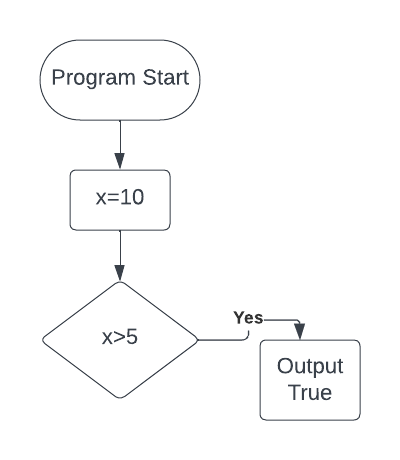
\includegraphics[scale=0.6]{./figures/flowchart1.png}
        \end{center}
    \end{minipage}
    \begin{minipage}[]{0.3\textwidth}
        \begin{center}
            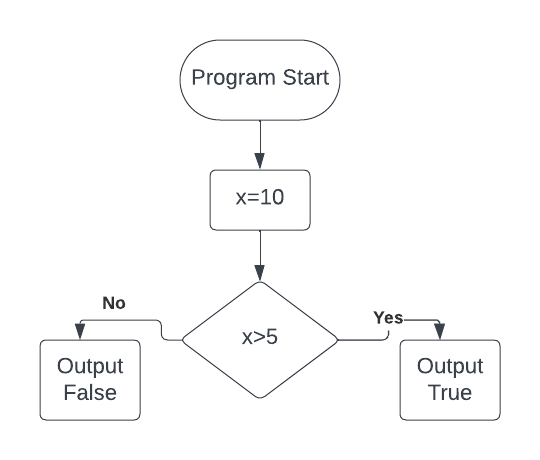
\includegraphics[scale=0.6]{./figures/flowchart2.png}
        \end{center} 
    \end{minipage}
    \begin{minipage}[]{0.3\textwidth}
        \begin{center}
            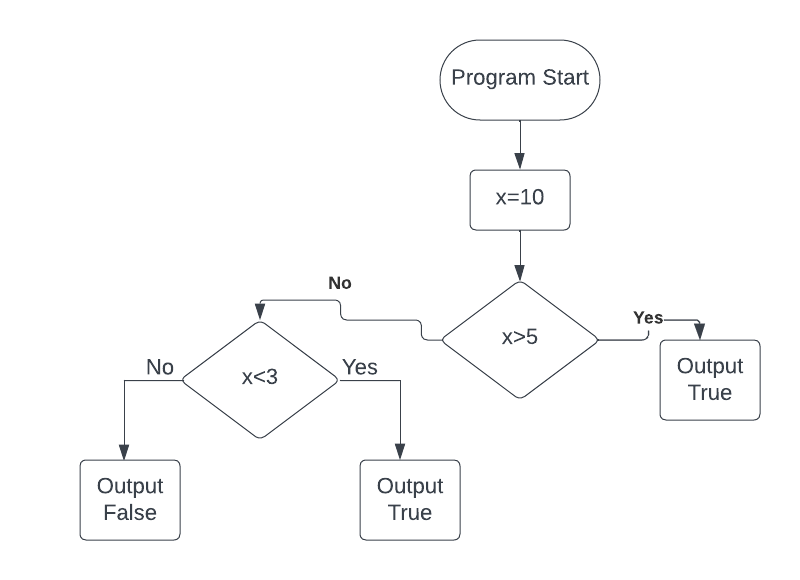
\includegraphics[scale=0.5]{./figures/flowchart3.png}
        \end{center} 
    \end{minipage}


    \bigbreak \noindent 
    \subsection{The Conditional Operator (Ternary)} 
    \bigbreak \noindent 
    \begin{concept}
 You can use the \textbf{conditional operator} to create short expressions that work like if/else statements. The general syntax is as follows:
	\end{concept}
    \smallbreak \noindent
    
    \begin{cppcode}
                            ( condition ) ? Statement_if_true :  statement_if_false
    \end{cppcode}
    
    \bigbreak \noindent 
    For example:
    \smallbreak \noindent
    
    \begin{cppcode}
( x < 0 ) ? y = 10 : z = 20;  

// Equivalent To
if (x < 0) {
    y = 10;
}else {
    z = 20;
}
    \end{cppcode}
    

    \pagebreak
    \subsection{Switch}
    \bigbreak \noindent 
    \begin{concept}
 The \textbf{switch} statement lets the value of a variable or an expression determine where the program will branch. IMPORTANT: Switch can \textbf{ONLY} be used for integers or characters
	\end{concept}
    \bigbreak \noindent 
    The general syntax for the switch statement is as follows:
    \bigbreak \noindent 
    
    \begin{cppcode}
switch (value){
    case some_case:
        statements;
        break

    case some_other_case:
        statements;
        break

    default:
        cout << "Cases not matched";
}
    \end{cppcode}
    
    \bigbreak \noindent 
    \nt{With switch, if we have a default block, it is important that we have a \textbf{break} statement in each case block, say a case is matched and we enter into the block, once the program exits the case block, it will continue on with the rest of the cases. Thus, the default will be triggered.}
    
    \bigbreak \noindent 
    Here is an example of switch:
    \bigbreak \noindent 
    
    \begin{cppcode}
const int x = 10;

switch (x) {
    case 5:
        std::cout << "5";
        break

    case 10:
        std::cout << "10";

    default:
        std::cout << "No Match";
}
    \end{cppcode}
    
    \bigbreak \noindent 
    \nt{The switch statement in C++ expects constant integral expressions for its case labels. In other words, the value for each case must be known at compile time and cannot be a variable or an expression that involves variables.}

    \pagebreak
    \unsect{The While Loop}
    \bigbreak \noindent 
    The general syntax for the C++ while loop is as follows:
    \bigbreak \noindent 
    
    \begin{cppcode}
while (expression)
    statement;
// or
while (expression) {
    statements;
}
    \end{cppcode}
    
    \bigbreak \noindent 
    \begin{minipage}[]{0.47\textwidth}
        Let's take a look a flowchart that describes a while loop:
    \end{minipage}
    \begin{minipage}[]{0.47\textwidth}
        \incfig{while}
    \end{minipage}
    \bigbreak \noindent 
    \nt{The while loop is know as a \textbf{pretest loop}, this is because its nature of testing the condition \textit{before} each iteration}

    \pagebreak
    \unsect{The Do-While Loop}
    \bigbreak \noindent 
    \begin{concept}
 The do while loop is a \textbf{posttest} loop which means its expression is tested after each iteration. Below is the general syntax for the do-while loop in C++:
	\end{concept}
    \bigbreak \noindent 
    
    \begin{cppcode}
do 
    statement
while (expression);

// or 

do {
    statements;
} while (expression);
    \end{cppcode}
    
    \bigbreak \noindent 
    \begin{minipage}[]{0.47\textwidth}
        Let's take a look at a simple flowchart that describes this concept.
    
    \end{minipage}
    \begin{minipage}[]{0.47\textwidth}
        \incfig{dowhlie3}
    \end{minipage}

    \pagebreak
    \unsect{The for loop}
    \bigbreak \noindent 
    \begin{concept}
 There are two types of loops, \textbf{conditional loops} and \textbf{count-controlled loops}. The for loop demonstrates a count-controlled loop, this type of loop is ideal for performing a known number of iterations.
	\end{concept}
    \bigbreak \noindent 
    The general syntax for the for loop is as follows
    \bigbreak \noindent 
    
    \begin{cppcode}
for (initialization; test; update)  
    statement;

// or

for (initialization; test; update) { 
    statements;
}
    \end{cppcode}
    

    \bigbreak \noindent 
    \nt{It is valid syntax to execute more than one statement in the initialization expression and the update expression. Additionally, the initialization stage of the for loop declaration if has already been preformed or if no Initialization is needed.}
    \bigbreak \noindent 
    below is an example of a for loop without the initialization stage.
    \bigbreak \noindent 
    
    \begin{cppcode}
int x=0;
for ( ; x < 10; ++x) {
    statements;
}

    \end{cppcode}
    
    \bigbreak \noindent 
    You may also omit the update stage of the for loop header if it will be preformed elsewhere in the loop body. In fact, you can even go as far as omitting all three expressions in loops parenthesis.

    \pagebreak
    \unsect{Using Files for Data Storage}
    \bigbreak \noindent 
    \begin{concept}
 When a program needs to save data for later use, it writes the data in a file. The data can then be read from the file at a later time.
	\end{concept}
    \bigbreak \noindent 
    \subsection{File Access Methods}
    \bigbreak \noindent 
    There are two general ways to access data stored in a file: \textit{sequential access} and \textit{direct access}. When you work with \textit{sequential-access file}, you access data from the beginning of the file to the end of the file.
    \bigbreak \noindent 
    When you work with a \textit{direct-access file}, you can jump to any piece  of data within the file without reading the data that comes before it.
    \bigbreak \noindent 
    \subsection{Setting up a program for file input/output}
    \bigbreak \noindent 
    In order for us to use file stream objects, we must include <fstream>.
    \bigbreak \noindent 
    
    \begin{cppcode}
#include <fstream>
    \end{cppcode}
    
    \bigbreak \noindent 
    \subsection{File Stream Objects}
    \bigbreak \noindent 
    In order for a program to work with a file on the computer's disk, the program must create a file stream object in memory. A \textit{file stream object} is an object that is associated with a specific file and provides a way for the program to work with that file. 
    \bigbreak \noindent 
    \textbf{File Stream Objects:}
    \begin{itemize}
        \item ofstream: we use this object when we want to create a file and write to it
        \item ifstream: we use this object when we want to open an existing file and read from it
        \item fstream: we use this object when we want to either read or write to a file
    \end{itemize}

    \pagebreak
    \subsection{Creating a file object and opening a file}
    \bigbreak \noindent 
    Before data can be written to or read from a file, the following things must happen:
    \begin{itemize}
        \item A file stream object must be created
        \item The file must be opened and linked to the file stream object
    \end{itemize}
    \bigbreak \noindent 
    The following example shows how to open a file for input (reading):
    \bigbreak \noindent 
    
    \begin{cppcode}
std::ifstream inputfile;
inputfile.open("filename.txt");

// Or just
std::ifstream inputfile("filename.txt");

// To read from the file... (assuming there are 2 lines of text)

std::string line1, line2;

inputfile >> line1;
cout << line1;

inputfile >> line2;
cout << line2;
    \end{cppcode}
    
    \bigbreak \noindent 
    The following example shows how to open a file for output (writing):
    \bigbreak \noindent 
    
    \begin{cppcode}
std::ofstream outputfile;
outputfile.open("filename.txt");

// Or just
std::ofstream outputfile("filename.txt");

// To write to the file...
outputfile << "Some text \n";

// This...
string a{" "};
std::ofstream file("./myfile2");

if (file) {
    while (cin >> a && a!="q") {
        file << a << endl;
    }
}

file.close();
    \end{cppcode}
    

    \bigbreak \noindent 
    \subsection{Closing a file}
    \bigbreak \noindent 
    To close a file we write:
    \bigbreak \noindent 
    
    \begin{cppcode}
fileobject.close()
    \end{cppcode}
    

    \pagebreak
    \subsection{Reading from a file with an unknown number of lines}
    \bigbreak \noindent 
    We we use the >> operator to read from a file, it will return either 0 1 depending on if there was any content to read. Thus, we can use a while loop to avoid any errors.
    \bigbreak \noindent 
    
    \begin{cppcode}
while (inputfile >> line){
    cout << line << endl;
}
    \end{cppcode}
    

    \bigbreak \noindent 
    \subsection{Testing for file open errors}
    \bigbreak \noindent 
    Under certain circumstances, the open member function will not work. For example, the following code will fail if the file info.txt does not exist:
    \bigbreak \noindent 
    
    \begin{cppcode}
ifstream inputfile;
inputfile.open("info.txt");
    \end{cppcode}
    
    \bigbreak \noindent 
    To circumvent this problem, we can use a if statement to check if the file has been opened successfully:
    \bigbreak \noindent 
    
    \begin{cppcode}
ifstream inputfile("info.txt");
if (inputfile){
    statements;
}

// Or
if (inputfile.fail()) {
    cout << "failed";
}
    \end{cppcode}
    

    \pagebreak
    \unsect{rvalues and lvalues}
    \bigbreak \noindent 
    In C++, values are categorized as either lvalues or rvalues, which play a fundamental role in understanding expressions, value categories, and reference binding in the language.
    \bigbreak \noindent 
    Here's a simplified explanation:

    \bigbreak \noindent 
    \subsection{rvalue (right value):}
    \bigbreak \noindent 
    \begin{enumerate}
        \item \textbf{Temporary} rvalues often represent temporary values that don't have a specific location in memory (i.e., you can't take their address in a straightforward manner). They are typically values that you can't assign to, like a temporary result of an expression.
        \item \textbf{Examples:}
        \begin{itemize}
            \item Literals: 5, true, 'a'
            \item Results of most expressions: x + y, std::move(x)
        \end{itemize}
    \item \textbf{Binding:} You can't bind an rvalue to a regular (lvalue) reference (T\&). However, C++11 introduced rvalue references (T\&\&) which can bind to rvalues. This is fundamental for move semantics and perfect forwarding.
    \end{enumerate}

    \bigbreak \noindent 
    \subsection{lvalue}
    \bigbreak \noindent 
    \begin{enumerate}
        \item \textbf{Location:} An lvalue represents an object that occupies a specific, identifiable location in memory. You can think of lvalues as "things with a name."
        \item \textbf{Examples:}
            \begin{itemize}
                \item Variables: int x;
                \item Dereference of a pointer: *p
                \item Array subscript: arr[5]
            \end{itemize}
        \item \textbf{Binding:} An lvalue can be bound to an lvalue reference (T\&).
    \end{enumerate}







    \pagebreak
    \unsect{Breaking and Continuing a loop}
    \bigbreak \noindent 
    \begin{concept}
 The \textbf{break} statement causes a loop to terminate early. The \textbf{continue} statement causes it to stop the current iteration and jump to the next one.
	\end{concept}

    \pagebreak
    \unsect{Functions}
    \bigbreak \noindent 
    Functions in c++ are pretty simple, here is an example:
    \bigbreak \noindent 
    
    \begin{cppcode}
void myfunc() {
    statements;

}
int main(int argc, const char *argv[]){ myfunc(); return EXIT_SUCCESS; }
    \end{cppcode}
    
    \bigbreak \noindent 
    Where the type before the function identifier is the value that the function shall return.
    \bigbreak \noindent 
    \subsection{Function prototypes (function declarations)}
    \bigbreak \noindent 
    \begin{concept}
 A function prototype eliminates the need to place a function definition before all calls to the function.
	\end{concept}
    \bigbreak \noindent 
    Example:
    \bigbreak \noindent 
    
    \begin{cppcode}
void foobar();

void foobar() {
    statements;

}
int main(int argc, const char *argv[]){ foobar(); return EXIT_SUCCESS; }
    \end{cppcode}
    
    \bigbreak \noindent 
    \nt{Function definitions can be placed below \textit{main}, just prototype them above \textit{main}}
    
    \bigbreak \noindent 
    And we can add some parameters:
    \bigbreak \noindent 
    
    \begin{cppcode}
std::string foobar(std::string name) {
    return "Hello " + name;
}  

int main(int argc, const char *argv[]){ cout << foobar("nate") << endl; } // Hello nate 
    \end{cppcode}
    

    \pagebreak
    \subsection{Static locals}
    \bigbreak \noindent 
    Sometimes we don't want a local variable to be destroyed after the function call completes, in this case we can use the static keyword before the type in our variable declarations
    \bigbreak \noindent 
    
    \begin{cppcode}
int foobar() { static int num; return num++; }

int main(int argc, const char *argv[]) {
    std::cout << foobar() << std::endl; // 0
    std::cout << foobar() << std::endl; // 1
    std::cout << foobar() << std::endl; // 2

    return EXIT_SUCCESS;
}
    \end{cppcode}
    

    \bigbreak \noindent 
    We can also do default values, but these are trivial.

    \bigbreak \noindent 
    \subsection{PREREQ - Reference variables}
    \bigbreak \noindent 
    \begin{concept}
 A reference variable in C++ is an alias, or an alternative name, for an already existing variable. Once a reference is initialized to a variable, either the variable name or the reference name can be used to refer to the variable. Reference variables must be initialized, they cannot just be declared.
	\end{concept}
    \bigbreak \noindent 
    Example:
    \bigbreak \noindent 
    
    \begin{cppcode}
int a = 12;
int &b = a; 

cout << a << " " << b << endl; // 12 12

a = 15;
cout << a << " " << b << endl; // 15 15

b = 20; 
cout << a << " " << b << endl; // 20 20

    \end{cppcode}
    

    \pagebreak
    \subsection{Using reference variables as parameters}
    \bigbreak \noindent 
    \begin{concept}
 When used as parameters, reference variables allow a function to access the parameters original arguments. Changes to the parameter are also made to the arguments.
	\end{concept}
    \bigbreak \noindent 
    Example:
    \bigbreak \noindent 
    
    \begin{cppcode}
int foobar(int &refvar) { refvar *= 2; return refvar; }

int main(int argc, const char *argv[]) {
    
    int num = 5;

    cout << foobar(num) << endl;  // 10
    cout << foobar(num) << endl;  // 20

    return EXIT_SUCCESS;
}
    \end{cppcode}
    
    
    \bigbreak \noindent 
    \nt{You cannot pass lvalues to a function that takes a reference variable.}
    \bigbreak \noindent 

    \pagebreak
    \subsection{Overloading Functions}
    \bigbreak \noindent 
    \begin{concept}
 Two or more functions can have the same name, as long as their parameters are different.
	\end{concept}
    \bigbreak \noindent 
    Example:
    \bigbreak \noindent 
    
    \begin{cppcode}
int foobar(int x, int y) { return x + y; }

int foobar(int x, int y, int z) { return x + y + z; }

int main(int argc, const char *argv[]) {

    cout << foobar(1,2) << endl;
    cout << foobar(1,2,3) << endl;

    return EXIT_SUCCESS;
}
    \end{cppcode}
    

    \bigbreak \noindent \bigbreak \noindent 
    \subsection{The exit() function}
    \bigbreak \noindent 
    \begin{concept}

	\end{concept}
    \bigbreak \noindent 
    The \textbf{exit()} function causes a program to terminate, regardless of which function or control mechanism is executing.
    \bigbreak \noindent 
    \nt{the exit() function is defined in the cstdlib header}
    \bigbreak \noindent 
    The exit() function must be passed a integer value, usually 0 (EXIT\_SUCCESS), or 1 (EXIT\_FAILURE). We can also just pass the constants EXIT\_SUCCESS/EXIT\_FAILURE, (these constants are defined within cstdlib)
    Example:
    \bigbreak \noindent 
    
    \begin{cppcode}
exit(0);
exit(EXIT_SUCCESS);

exit(1);
exit(EXIT_FAILURE)
    \end{cppcode}
    

    \pagebreak
    \subsection{Stubs and Drivers}
    \bigbreak \noindent 
    \begin{concept}
 A \textbf{stub} is a \textit{dummy} function that is called instead of the actual function it represents. It usually displays a test message acknowledging that it was called, and nothing more.
	\end{concept}
    \bigbreak \noindent 
    Example:
    \bigbreak \noindent 
    
    \begin{cppcode}
int foobar(int x) {
    std::cout << "Function foobar was called with integer argument " 
    << x 
    << std::endl;
}
    \end{cppcode}
    
    \bigbreak \noindent 
    This allows for debugging by making sure the function was called at the correct time and with the correct arguments.
    \bigbreak \noindent 
    \begin{concept}
 A \textbf{driver} is a program that tests a function by simply calling it. If the function accepts arguments, the driver passes test data.
	\end{concept}

    \pagebreak
    \unsect{Arrays and Vectors}
    \bigbreak \noindent 
    \subsection{Arrays}
    \bigbreak \noindent 
    \begin{concept}
 An array allows you to store and work with multiple values of the same data type. An arrays size declaration must be a constant integer expression with a value greater than or equal to zero. The amount of memory that the array uses depends on the array's data type and the number of elements.
	\end{concept}
    \bigbreak \noindent 
    Example:
    \bigbreak \noindent 
    
    \begin{cppcode}
int arr[3]; // array of 3 integer elements
double arr[6]; // array of 6 double elements
int myarr[3] = {1,2,3};

// Getting the elements of an array
std::cout << myarr[0]; // Outputs first value (1)
    \end{cppcode}
    
    \bigbreak \noindent 
    \nt{Arrays are defined with braces}
    \bigbreak \noindent 

   \bigbreak \noindent 
   \subsection{Partial array initialization}
   \bigbreak \noindent 
   We can also only initialize part of an array. In the case of an integer array, the elements that we do not define will be set to zero. Other cases depend on the data type used.
   \bigbreak \noindent 
   
   \begin{cppcode}
int arr[5] = {1,2,3}; // {1,2,3,0,0}
   \end{cppcode}
   

   \bigbreak \noindent 
   \subsection{Implicit array sizing}
   \bigbreak \noindent 
   Its possible to define an array without specifying a size, as long as we provide an initialization list, c++ will automatically make the array large enough to hold all of the initialization values.

   \bigbreak \noindent 
   \subsection{Bound violation}
   \bigbreak \noindent 
   If we try to add values to a function without any remaining space, the program will crash.

   \pagebreak
   \subsection{The range based for loop}
   \bigbreak \noindent 
   \begin{concept}
 The \textbf{range-base for loop} is a loop that iterates once for each element in an array.
	\end{concept}
   \bigbreak \noindent 
   Example:
   \bigbreak \noindent 
   
    \begin{cppcode}
int lastindex;
lastindex = (sizeof(arr) / sizeof(arr[0])-1);
for (int i: arr)  {
    if (i != arr[lastindex]) {
        cout << i << ",";
    } else {
        cout << i;
    }
}
   \end{cppcode}
   

   \subsection{Modifying an array with a range-based for loop}
   \bigbreak \noindent 
   We can declare the range variable as a reference. This way, any change made to \textit{i} will be reflected in our array.
   \bigbreak \noindent 
   
   \begin{cppcode}
int arr[3] = {1,2,3};

for (int &i: arr)  {
    i = 5;
}

for (int i : arr) cout << i << " "; // 5 5 5
   \end{cppcode}
   

   \bigbreak \noindent 
   \subsection{Thou shall not assign}
   \bigbreak \noindent 
   It is crucial to understand  that we can not simply assign an array to some other array variable. The only way to copy over the array to a new variable is to use a loop. Whenever we refer to an array by just its identifier, we are only referring to its \textit{beginning memory address}.
   \bigbreak \noindent 
   A corollary to this concept would lead to the conclusion that we will also not be able to print the contents of an array by:
   \bigbreak \noindent 
   
   \begin{cppcode}
int arr[5] = {1,2,3,4,5};
std::cout << arr << std::endl;

   \end{cppcode}
   
   \bigbreak \noindent 
   This will only display the arrays \textbf{memory address}, we must use a loop to display the contents.

   \pagebreak
   \subsection{Getting the size of an array}
   \bigbreak \noindent 
   To get the size of the array, we can use the \textit{sizeof()} function. The way this works is we get the size of the entire array, and then divide by the size of any element.
   \bigbreak \noindent 
    
    \begin{cppcode}
int arr[3] = {1,2,3};
std::cout << sizeof(arr) / sizeof(arr[0]) << std::endl;  // 3

// We can also get the last index position by subtracting one
    std::cout << sizeof(arr) / sizeof(arr[0]) - 1 << std::endl;  // 3
    \end{cppcode}
    
    \bigbreak \noindent 

    \bigbreak \noindent 
    \subsection{Arrays as function arguments}
    \bigbreak \noindent 
    \begin{concept}
  To pass an array as an argument to a function, pass the name of the array. When we pass an array to a function, we are passing a reference to the array, this means any changes to the array in the function will be reflected to the array we passed.
	\end{concept}
    \bigbreak \noindent 
    
    \begin{cppcode}
int main(int argc, const char *argv[]) {

    const int SIZE = 3;
    int myarr[3] = {1,2,3};

    for (int i: myarr) cout << i << endl; // 1 2 3

    foobar(myarr, SIZE);

    for (int i: myarr) cout << i << endl; // 2 3 4



    return EXIT_SUCCESS;
}

void foobar(int arr[], int size) {

    for ( int i=0; i < size; ++i ) {
        arr[i]++;
    }


}
    \end{cppcode}
    

    \bigbreak \noindent 
    \nt{If we do not wish for a function to make any changes to the array argument, we must declare it as const in the function parameters.}

    \pagebreak
    \subsection{2D array (matrix)}
    \bigbreak \noindent 
    \begin{concept}
 A two-dimensional array is like sereval identical arrays put together. It is useful for storing multiple sets of data. In mathematics, this type of concept would be called a \textbf{matrix}
	\end{concept}
    \bigbreak \noindent 
    \begin{minipage}[]{0.47\textwidth}
    Consider the arrays:
    \begin{center}
        $A = \{a_{1}, a_{2}, a_{3}\} $ \\
        $a_{1} = \{1,2,3\} $ \\
        $a_{2} = \{4,5,6\} $ \\
        $a_{3} = \{7,8,9\} $ \\
    \end{center}
    \end{minipage}
    \begin{minipage}[]{0.47\textwidth}
    Then we have:
    \begin{align*}
        \begin{bmatrix}
            1 & 2 & 3 \\
            4 & 5 & 6 \\
            7 & 8 & 9
        \end{bmatrix}
    .\end{align*}
    \end{minipage}
    \bigbreak \noindent 
    So in C++, this would be:
    \bigbreak \noindent 
    
    \begin{cppcode}
int arr[3][3] = {{1,2,3}, {4,5,6}, {7,8,9}};
int arr[3][3] = {
                {1,2,3},
                {4,5,6},
                {7,8,9}
            };
// and we can index a matrix with
arr[row number][column number];
std::cout << arr[0][0];  // 1
    \end{cppcode}
    \bigbreak \noindent 
    The way we can output all elements of this matrix would look something like:
    \bigbreak \noindent 
    \begin{minipage}[t]{0.47\textwidth}
    \bigbreak \noindent 
    
    \begin{cppcode}

    const int SIZE = 3;
    int arr[3][3] = {
                {1,2,3},
                {4,5,6},
                {7,8,9}
            };

    for (int i{0}; i < SIZE; ++i) {
        for (int j{0}; j < SIZE; ++j) {
            cout << arr[i][j] << " ";
        } 
        cout << endl;
    }
    \end{cppcode}
    \end{minipage}
    \hspace{0.2in} 
    \begin{minipage}[t]{0.47\textwidth}
\bigbreak \noindent 
\begin{cppcode}
    const int ROW_SIZE = 3;
    const int COLUMN_SIZE = 4;
    int arr[ROW_SIZE][COLUMN_SIZE] = {
                {1,2,3},
                {4,5,6,6},
                {7,8,9}
            };

    for (int i{0}; i < ROW_SIZE; ++i) {
        for (int j{0}; j < COLUMN_SIZE; ++j) {
            cout << arr[i][j] << " ";
        } 
        cout << endl;
    }
\end{cppcode}
    \end{minipage}
    \bigbreak \noindent 
    

    \pagebreak
    \subsection{Passing a matrix to a function}
    \bigbreak \noindent 
    Unlike array parameter declarations not needing a size, matrix parameters do.
    \bigbreak \noindent 
    
    \begin{cppcode}
const int ROW_SIZE = 3;
const int COLUMN_SIZE = 4;

void foobar(const int arr[][COLUMN_SIZE], int row_size) {
    for (int i{0}; i < row_size; ++i) {
        for (int j{0}; j < COLUMN_SIZE; ++j) {
            cout << arr[i][j] << " ";
        }
        cout << endl;
    }
}

int main(int argc, const char *argv[]) {


    int arr[ROW_SIZE][COLUMN_SIZE] = {
                {1,2,3},
                {4,5,6,6},
                {7,8,9}
            };

    foobar(arr, ROW_SIZE);

    return EXIT_SUCCESS;
}
    \end{cppcode}
    

    \pagebreak
    \subsection{The STL Vector}
    \bigbreak \noindent 
    \textbf{Concept. } The \textit{Standard Template Library} offers a \textbf{vector} data type, which in many ways, is superior to standard arrays.
    \bigbreak \noindent 
    The STL is a collection of data types and algorithms that you may use in your programs. 
    \bigbreak \noindent 
    A \textbf{vector} is a container that can store data. It is like an array in the following ways:
    \begin{itemize}
        \item A vector holds a sequence of values.
        \item A vector stores its elements in a contiguous memory location.
        \item You can use the array subscript operator []
    \end{itemize}

    \bigbreak \noindent 
    \subsection{Defining a vector}
    \bigbreak \noindent 
    
    \begin{cppcode}
#include <vector>
std::vector<type> name(size); // size is optional 
// Examples
std::vector<int> a(3); // Vector of ints, size 3 with fill of zeros
std::vector<int> a(3, 2); // Vector of ints, size 3 with fill of twos
std::vector<int> a(othervector) // Copy of some other vector
std::vector<int> b = {1,2,3}; // Vector of ints
std::vector<int> b {1,2,3}; // Vector of ints
std::vector<int> b{1,2,3}; // Vector of ints
    \end{cppcode}
    
    \bigbreak \noindent 
    \nt{If we declare a size for the vector, we \textbf{cannot} define its elements in the same statement, defining elements of a vector in the same statement in which it's declared automatically defines its size, so manually doing is not only not needed, but will produce an error.}

    \bigbreak \noindent 
    \subsection{Get index position of elements}
    \bigbreak \noindent 
    To get the index position of an element in a vector, we can use the \textbf{at(\textit{pos})} member function.
    \bigbreak \noindent 
    Example:
    \bigbreak \noindent 
    
    \begin{cppcode}
std::vector<int> a {1,2,3};
cout << a.at(0); // 1
    \end{cppcode}
    

    \bigbreak \noindent 
    \subsection{Adding to a vector}
    \bigbreak \noindent 
    To store a value in a vector that does not have a starting size, or that is already full, use the \textbf{push\_back()} member function. This function accepts an element and stores it at the end of the vector.
    \bigbreak \noindent 
    Example:
    \bigbreak \noindent 
    
    \begin{cppcode}
std::vector<int> a {1,2,3};
a.push_back(4);
    \end{cppcode}
    

    \bigbreak \noindent 
    \subsection{Getting the size of a vector}
    \bigbreak \noindent 
    To get the size of a vector, we can use the \textbf{size()} member function.
    \bigbreak \noindent 
    Example:
    \bigbreak \noindent 
    
    \begin{cppcode}
std::vector<int> a {1,2,3};
std::cout << size(a) << std::endl;  // 3
    \end{cppcode}
    

    \bigbreak \noindent 
    \subsection{Removing last element of a vector} 
    \bigbreak \noindent 
    To remove elements from a vector, we can utilize the \textbf{pop\_back()} member function. This function will remove the last element of the vector.
    \bigbreak \noindent 
    Example:
    \bigbreak \noindent 
    
    \begin{cppcode}
std::vector<int> a {1,2,3};
a.pop_back(); // Removes the last element (3).
    \end{cppcode}
    

    \bigbreak \noindent 
    \subsection{Removing elements of a vector }
    \bigbreak \noindent 
    To remove elements:
    \bigbreak \noindent 
    
    \begin{cppcode}
std::vector<int> myvec{1,2,3,4};
myvec.erase(myvec.begin() + 1); // Removes the second element (2)
    \end{cppcode}
    

    \bigbreak \noindent 
    \subsection{Clearing a vector}
    \bigbreak \noindent 
    To clear a vector we can use the \textbf{clear()} member function.
    \bigbreak \noindent 
    Example:
    \bigbreak \noindent 
    
    \begin{cppcode}
std::vector<int> a {1,2,3};
a.clear();
    \end{cppcode}
    

    \bigbreak \noindent 
    \subsection{Detecting an Empty vector}
    \bigbreak \noindent 
    To determine if a vector is empty, we can use the \textbf{empty()} function. This function will return 0 or 1 depending on whether the vector contains any elements.
    \bigbreak \noindent 
    Example:
    \bigbreak \noindent 
    
    \begin{cppcode}
std::vector<int> a {1,2,3};
std::vector<int> b;
cout << a.empty(); // 0
cout << b.empty(); // 1
    \end{cppcode}
    

    \bigbreak \noindent 
    \subsection{Resizing a vector}
    \bigbreak \noindent 
    To resize a vector, we can use the \textbf{resize()} member function.
    \bigbreak \noindent 
    Example:
    \bigbreak \noindent 
    
    \begin{cppcode}
std::vector<int> a {1,2,3};
a.resize(5,2); // resize the vector to a total size of 5 elements, filling with 2s.
a.resize(5); // resize the vector to a total size of 5 elements, filling with 0s.
    \end{cppcode}
    

    \bigbreak \noindent 
    \subsection{Swapping Vectors}
    \bigbreak \noindent 
    To swap the contents of two vectors, we can use the \textbf{swap(\textit{vector})} member function.
    \bigbreak \noindent 
    Example:
    \bigbreak \noindent 
    
    \begin{cppcode}
std::vector<int> v1 {1,2,3};
std::vector<int> v2 {4,5,6};

v1.swap(v2);
    \end{cppcode}
    

    \pagebreak
    \unsect{Searching and Sorting Arrays}
    \bigbreak \noindent 
    \begin{concept}
 A search algorithm is a method of locating a specific item in a larger collection of data. This section discusses two algorithms for searching the contents of an array.
	\end{concept}
    \bigbreak \noindent 
    \subsection{The linear search}
    \bigbreak \noindent 
    The linear search is very simple, it uses a loop to sequentially step through an array, starting with the first element.
    \bigbreak \noindent 
    Example:
    \bigbreak \noindent 
    
    \begin{cppcode}
int main(int argc, const char *argv[]) {

    const int SIZE = 5;
    int arr[SIZE] = {88,67,5,23,19};

    int target = 5;

    for (int i{0}; i <= SIZE + 1; ++i) {
        if (i == SIZE + 1) {
            cout << "Target not in array" << endl;
        }
        if ( arr[i] == target ) {
            cout << "Target [" << target << "] found at index position " << i << endl;
            break;
        }
    }
    return EXIT_SUCCESS;
}
    \end{cppcode}
    
    \bigbreak \noindent 
    
    \begin{cppcode}
int linearsearch(int arr[], int size, int target) {
    int index{0}, position{-1};
    bool found = false;

    while (index < size && !found) {
        if (arr[index] == target) {
            position = index;
            found = true;
        }
        ++index;
    }
    return position;
}
    \end{cppcode}
    
    \bigbreak \noindent 
    \pagebreak
    One drawback to the linear search is its potential inefficiency, its quite obvious to notice that for large arrays, the linear search will take a long time, if an array has 20,000 elements, and the target is at the end, then the search will have to compare 20,000 elements.
    \bigbreak \noindent 
    \subsection{The binary search}
    \bigbreak \noindent 
    The binary search algorithm is a clever approach to searching arrays. Instead of testing the array's first element, the algorithm starts with the leement in the middle. If that element happens to contain the desired value, then the search is over. Otherwise, the value in the middle element is either greater than or less than the value being searched for. If it is greater, then the desired value (if it is in the array), will be found somewhere in the first half of the array. If it is less, then the desired value, it will be found somewhere in the last half of the array. In either case, half of the array's elements have been eliminated from further searching.
    \bigbreak \noindent 
    \nt{The binary search algorithm requires the array to be sorted.}
    \bigbreak \noindent 
    Example:
    \bigbreak \noindent 
    
    \begin{cppcode}
int binarysearch(int arr[], int size, int target) {
    int first{0}, 
        middle,
        last = size -1,
        position{-1};

    bool found = false;

    while (!found && first <= last) {
        middle = (first + last) / 2;
        if (arr[middle] == target) {
            found = true;
            position = middle;
        } else if (target > arr[middle]) {
            first = middle + 1;
        } else {
            last = middle - 1;
        }
    }
    return position;
}
    \end{cppcode}
    
    \bigbreak \noindent 
    Powers of twos are used to calculate the max number of comparisons the binary search will make on an array. Simply find the smallest power of 2 that is greater than or equal to the number of elements in the array. For example:
    \bigbreak \noindent 
    \begin{minipage}[]{0.47\textwidth}
    \begin{align*}
        n = 50,000 \\
        2^{15} = 32,768 \\
        2^{16} = 65,536
    .\end{align*}
    \end{minipage}
    \begin{minipage}[t]{0.47\textwidth}
        Thus, there are a maximum of 16 comparisons for a array of size 50,000
    \end{minipage}

    \pagebreak
    \subsection{Bubble Sort}
    \bigbreak \noindent 
    The bubble sort algorithm makes passes through and compares the elements of the array, certain values "bubble" toward the end of the array with each pass.
    \bigbreak \noindent 
    Example:
    \bigbreak \noindent 
    
    \begin{cppcode}
void swap(int &a, int &b) {
    int temp = a;
    a = b;
    b = temp;
}

void bubblesort(int arr[], int size) {

    for (int max = size; max > 0; --max) {
        for (int i{0}; i < size; ++i) {
            if (arr[i] > arr[i + 1]) {
                swap(arr[i], arr[i+1]);
            }
        }
    } 
}
    \end{cppcode}
    

    \bigbreak \noindent 
    \subsection{Selection Sort}
    \bigbreak \noindent 
    The bubble sort algorithm is simple, but it is ineffective because values move by only one element at a time toward their final destination in the array. The \textit{selection sort algorithm} usually performs fewer swaps because it moves items immediately to their final position in the array. 
    \bigbreak \noindent 
    Example:
    \bigbreak \noindent 
    
    \begin{cppcode}
void swap(int &a, int &b) {
    int temp = a;
    a = b;
    b = temp;
}

void selectionsort(int arr[], int size) {


    for(int j=0; j < size; ++j) {
        int &minelement = arr[j];
        for (int k = j+1; k < size; ++k) {
            if ( arr[k] < minelement ) {
                swap(minelement, arr[k]);
            }
        }

    }
}
    \end{cppcode}
    

    \pagebreak
    The selection sort starts with the assumption that the first element is already the smallest, then it scans the array and tries to find a smaller value. If one is found, it moves that element to the front. Once the iteration is complete, we can be sure that the smallest value is at the front and +1 is added to the loop index.

    \pagebreak
    \unsect{Pointers}
    \bigbreak \noindent 
    \begin{concept}
 Pointers are variables that store the memory address of a variable, we can use the \& operator to retrieve the address of a variable. Pointers are like references, any changes we make to the variable the holds the pointer, the change will be reflected in the original variable.
	\end{concept}
    \bigbreak \noindent 
    \nt{In order to access the contents of a pointer, we must \textbf{dereference}, more on this later.}
    
    \bigbreak \noindent 
    Example:
    \bigbreak \noindent 
    
    \begin{cppcode}
int a = 12;
int *b; // Initialize pointer  
b = &a; // Get the memory address of a and store in b
cout << b; // Output the memory address
cout << *b; // Output the contents
*b = 15; // Change the value of b, change reflected to a
// We can also put the asterisk next to the type
int* b;
    \end{cppcode}
    

    \bigbreak \noindent 
    \subsection{Nullptr}
    \bigbreak \noindent 
    It is never a good idea to use an uninitialized pointer, this could mean we are affecting some random memory address. To circumvent this, we can use the bulitin keyword \textit{nullptr}. Assigning a pointer to nullptr means we are assigning it to the address zero. When we do this, we say that the pointer points to "nothing".
    \bigbreak \noindent 
    
    \begin{cppcode}
int* b = nullptr;
    \end{cppcode}
    
    \bigbreak \noindent 
    \nt{If we try to deference the contents of a nullptr, we will get \textbf{address boundary error} at runtime}
    
    \pagebreak
    \subsection{Arrays as pointers}
    \bigbreak \noindent 
    \begin{concept}
 Array names can be used as constant pointers, and pointers can be used as array names.
	\end{concept}
    \bigbreak \noindent 
    We have already discussed that referencing an array without the subscript operator returns the address of the beginning of the array. Thus, we can conclude that an array is just a \textit{pointer} to the first element.
    \bigbreak \noindent 
    If we deference an array, we can get access to the first element.
    \bigbreak \noindent 
    
    \begin{cppcode}
int arr[3] = {1,2,3};
cout << *arr << endl; // 1
    \end{cppcode}
    
    \bigbreak \noindent 
    We can gain access to the other elements via some simply arithmetic:
    \bigbreak \noindent 
    
    \begin{cppcode}
int arr[3] = {1,4,3};
cout << *(arr+1); // 4
    \end{cppcode}
    
    \bigbreak \noindent 
    We we add one to \textit{arr}, we are actually adding 1 multiplied by the size of the data type that we are trying to access. This allows us to change the address of the first element to the address of the second.
    \bigbreak \noindent 
    Therefore, we can generalize:
    \bigbreak \noindent 
    
    \begin{cppcode}
arr[index] = *(arr + index)
    \end{cppcode}
    

    \bigbreak \noindent 
    We can assign pointers to arrays
    \bigbreak \noindent 
    
    \begin{cppcode}
int arr[3] = {1,2,3};
int* b = arr;
cout << *b << endl; // 1
for (int i{0}; i < 3; ++i) {
    cout << b[i] << endl;
}
    \end{cppcode}
    

    \pagebreak
    \subsection{Pointers as Function Parameters}
    \bigbreak \noindent 
    We can also declare pointer parameters in functions, giving the function access to the original variable, much like reference
    \bigbreak \noindent 
    
    \begin{cppcode}
void foobar(int* pt) {
    *pt = 5;
}

int a = 10;
foobar(&a); // Changes a to the value 5

    \end{cppcode}
    

    \bigbreak \noindent 
    \subsection{Pointers to constants}
    \bigbreak \noindent 
    Sometimes, it is necessary to pass the address of a const item into a pointer. When this is the case, the pointer must be defined as a pointer to a const item.
    \bigbreak \noindent 
    
    \begin{cppcode}
const int* b; 
const int *b;
    \end{cppcode}
    
    \bigbreak \noindent 
    \nt{It should be noted that the keyword const is referring to the thing that $b$ is pointing to, not $b$ itself. Furthermore, it is crucial that we have the const modifier on line 2, if we are trying to point to a constant, then this is required. This does not mean the thing we are trying to point to needs the const qualifier for line 2 to be valid. lastly, because $b$ is a pointer to a const, the compiler will not allow us to write code that changes the thing that $b$ points to.}
    \bigbreak \noindent 

    \pagebreak
    \subsection{Constant Pointers}
    \bigbreak \noindent 
    We can also use the const key word to define a constant pointer. Here are the differences:
    \begin{itemize}
        \item A pointer to a const points to a constant item. The data that the pointer points to cannot change, but the pointer itself can change. 
        \item With a const pointer, it is the pointer itself that is constant.  Once the pointer is initialized with an address, it cannot point to anything else.
    \end{itemize}
    \bigbreak \noindent 
    Example:
    \bigbreak \noindent 
    
    \begin{cppcode}
int* const ptr;
int *const ptr;
    \end{cppcode}
    

    \bigbreak \noindent 
    \subsection{Both pointer to constant and constant pointer}
    \bigbreak \noindent 
    
    \begin{cppcode}
const int* const ptr;
const int *const ptr;
    \end{cppcode}
    

    \bigbreak \noindent 
    \subsection{Prereq - Static vs Dynamic memory allocation}
    \bigbreak \noindent 
    There are different types of memory allocation in a C++ program. By default, creating variables will utilize "static memory allocation", this is where variables are created on the "stack". The stack is a region of memory where local variables, function parameters, return addresses, and control flow data are stored. It operates in a Last-In-First-Out (LIFO) manner.
    \bigbreak \noindent 
    When a function is called, a new "stack frame" is pushed onto the stack. This frame contains the function's local variables, parameters, and the return address.
    When the function returns, its stack frame is popped off, and the stack pointer moves back to the previous frame.
    The stack grows and shrinks automatically as functions are called and return.
    \bigbreak \noindent 
    \textbf{Characteristics:}
    \begin{itemize}
        \item \textbf{Automatic Memory Management:} Memory allocation and deallocation on the stack are automatic. When a function exits, its local variables are automatically deallocated.
        \item \textbf{Speed:} Stack operations (push and pop) are very fast.
        \item \textbf{Fixed Size:} The stack has a fixed size, determined at the start of the program. If a program uses more stack space than is available (e.g., due to deep or infinite recursion), it will result in a "stack overflow."
    \end{itemize}
    \bigbreak \noindent 
    In constrast to this, we also have \textbf{dynamic memory allocation}: In has the following characteristics:
    \begin{itemize}
        \item Memory is allocated during runtime.
        \item Uses functions like malloc(), calloc(), realloc(), and new (in C++) to allocate memory.
        \item Requires manual deallocation using functions like free() or delete (in C++).
        \item Memory is allocated on the heap.
        \item The size of the memory allocation can be determined at runtime based on program needs.
    \end{itemize}



    \bigbreak \noindent 
    \subsection{Dynamic Memory Allocation}
    \bigbreak \noindent 
    \begin{concept}
 Variables may be created and destroyed while a program is running.
	\end{concept}
    \bigbreak \noindent 
    In the cases where we don't know how many variables we will need for a program, we can allow a program to create its own variables "on the fly". This is called \textit{dynamic memory allocation} and this is only possible through pointers.
    \bigbreak \noindent 
    To dynamically allocate memory means that a program, while running, asks the computer
to set aside a chunk of unused memory large enough to hold a variable of a specific data
type. Let’s say a program needs to create an integer variable. It will make a request to the
computer that it allocate enough bytes to store an int. When the computer fills this request,
it finds and sets aside a chunk of unused memory large enough for the variable. It then gives
the program the starting address of the chunk of memory. The program can only access the
newly allocated memory through its address, so a pointer is required to use those bytes.

    \bigbreak \noindent 
    The way a C++ program requests dynamically allocated memory is through the new operator. Assume a program has a pointer to an int defined as
    \bigbreak \noindent 
    
    \begin{cppcode}
int *ptr = nullptr;
// Then we can do:
ptr = new int;
// A value may be stored in this new variable by dereferencing the pointer:
*ptr = 15;
    \end{cppcode}
    

    \bigbreak \noindent 
    This statement is requesting that the computer allocate enough memory for a new int variable. The operand of the new operator is the data type of the variable being created. Once the statement executes, ptr will contain the address of the newly allocated memory. Then we store a value in the new variable by dereferencing.
    \bigbreak \noindent 
    Although the statements above illustrate the use of the new operator, there’s little purpose
in dynamically allocating a single variable. A more practical use of the new operator is to
dynamically create an array. Here is an example of how a 100-element array of integers
may be allocated:
\bigbreak \noindent 

\begin{cppcode}
ptr = new int[100];
\end{cppcode}

\bigbreak \noindent 
    Once the array is created, the pointer may be used with subscript notation to access it. 

    \bigbreak \noindent 
     it should
release it for future use. The delete operator is used to free memory that was allocated
with new. Here is an example of how delete is used to free a single variable, pointed to
by iptr :
    \bigbreak \noindent 
    
    \begin{cppcode}
delete ptr;
ptr = nullptr; // Always set to nullptr after deleting
delete [] ptr; // If ptr points to a dynamically allocated array
ptr = nullptr; // Always set to nullptr after deleting
    \end{cppcode}
    
    \bigbreak \noindent 
    \nt{Failure to release dynamically allocated memory can cause a program to have a memory leak. Only use pointers with delete that were previously used with new. If you use a pointer with delete that does not reference dynamically allocated memory, unexpected problems could result!}
    \bigbreak \noindent 

    \bigbreak \noindent 
    \subsection{When to use DMA}
    \bigbreak \noindent 
    \begin{enumerate}
        \item Memory Location: The integer is allocated on the heap.
        \item Lifetime: The memory remains allocated until it's explicitly deallocated using delete.
        \item Use Cases:
        \begin{itemize}
            \item Variable Size: When you need data structures of variable size, like linked lists or dynamic arrays.
            \item Long-lived Objects: When you need objects that outlive the function they were created in.
            \item Avoiding Stack Overflow: For large allocations, the stack might not have enough space, leading to stack overflow. In such cases, DMA is preferred.
            \item For Polymorphism: In object-oriented programming, DMA is often used with pointers to base and derived classes to achieve polymorphism.
        \end{itemize}
    \end{enumerate}

    \bigbreak \noindent 
    \subsection{Returning pointers from a function}
    \bigbreak \noindent 
    \begin{concept}
 Functions can return pointers, but you must be sure the item the pointer references still exists.
	\end{concept}
    \bigbreak \noindent 
    We should return  a pointer from a function only if it is:
    \begin{itemize}
        \item A pointer to an item that was passed into the function as an argument.
        \item A pointer to a dynamically allocated chuck of memory
    \end{itemize}

    \bigbreak \noindent 
    \subsection{Smart Pointers}
    \bigbreak \noindent 
    \begin{concept}
 C++ 11 introduces smart pointers, objects that work like pointers, but have the ability to automatically delete dynamically allocated memory that is no longer being used.
	\end{concept}
    \bigbreak \noindent 
    We have three types:
    \begin{itemize}
        \item \textbf{unique\_ptr}: The sole owner of a piece of dynamically allocated memory. 
        \item \textbf{shared\_ptr}: Can share ownership of a piece of dynamically allocated memory. Multiple pointers of the shared\_ptr type can point to the same piece of memory
        \item \textbf{weak\_ptr}: Does not own the memory it points to, and cannot be used to access the memory's contents. Used when the memory pointed to by a shared\_ptr must be referenced without increasing the number of shared\_ptrs that own it.
    \end{itemize}
    \bigbreak \noindent 
    \nt{To use these smart pointers, we must include <memory>}

    \pagebreak
    Here is the syntax for a unique pointer:
    \bigbreak \noindent 
    
    \begin{cppcode}
unique_ptr<type> name( new type );
// Example
std::unique_ptr<int> a( new int ); // Basic way 
std::unique_ptr<int> a = std::make_unique<int>(15); // Preferred Way (Initialization of 15)
std::unique_ptr<int> a = std::make_unique<int>(); // Preferred Way (initialization of zero)
std::shared_ptr<int> b = a; //  NOT VALID, unique_ptr must be unique
    \end{cppcode}
    
    \bigbreak \noindent 
    So now we have two entities: a \textbf{unique\_ptr} located on the \textit{stack} and an \textbf{int} located on the \textit{heap}. The unique\_ptr holds the address of the int we created on the heap. Since this is a \textbf{smart pointer}, the integer object will be deleted and the unique pointer that was holding the memory address will be set to nullptr will be deleted and the unique pointer that was holding the memory address will be set to \textbf{nullptr}.
    \bigbreak \noindent 
    A \textbf{shared\_ptr} works via a \textbf{reference counter} maintained in a control block. This mechanism keeps track of how many shared\_ptr instances are pointing to the same object. Once the reference count reaches zero, the managed object is deleted. The control block also tracks weak references and is deallocated when both shared and weak counts reach zero. Here is how we build such object:
    \bigbreak \noindent 
    
    \begin{cppcode}
std::shared_ptr<type> identifier( new int ); // Basic Way
std::shared_ptr<type> identifier = std::make_shared<type>(initialization); // Preferred Way
// Example
std::shared_ptr<int> a( new int );
std::shared_ptr<int> a = std::make_shared<int>(10);
std::shared_ptr<int> b = a; // Valid copy
    \end{cppcode}
    

    \bigbreak \noindent 
    Lastly, we can define a \textbf{weak\_ptr}, we can assign this object to any shared\_ptr object, but the reference count will not be updated.
    \bigbreak \noindent 
    
    \begin{cppcode}
std::shared_ptr<int> a = std::make_shared<int>(10);
std::weak_ptr<int> b = a; // Reference count will NOT be updated.
    \end{cppcode}
    

    \pagebreak
    \unsect{Characters, C-Strings and more about the string class}
    \bigbreak \noindent 
    \subsection{Character Testing}
    \bigbreak \noindent 
    The C++ library provides several functions that allaw us to test the value of a character. These functions test a single \textit{char} argument and return either true or false.
    \bigbreak \noindent 
    To use these functions, we must include <cctype>
    \begin{itemize}
        \item isalppha
        \item isalnum
        \item isdigit
        \item islower
        \item isprint
        \item ispunct
        \item isupper
        \item isspace
    \end{itemize}

    \bigbreak \noindent 
    \subsection{Character case conversion}
    \bigbreak \noindent 
    We also have functions for converting characters to uppercase or lowercase.
    \begin{itemize}
        \item toupper
        \item tolower
    \end{itemize}

    \bigbreak \noindent 
    \subsection{C Strings }
    \bigbreak \noindent 
    \begin{concept}
 A C-string is a sequence of characters stored in consecutive memory locations, terminated by a null character. In C++, all string literals are stored in memory as C-Strings. The purpose of  a \textbf{null terminator} is to mark the end of the C-String.
	\end{concept}
    \bigbreak \noindent 
    It's important to realize that a string literal has its own storage location, just like a variable or an array. When a string literal appears in a statement, it's actually its memory address that C++ uses. 

    \pagebreak
    \subsection{C-Strings stored in arrays}
    \bigbreak \noindent 
    In C, there is no string class that we can use, so when a C programmer wants to create a string, they must make a char array to house it. The char array must be large enough to house the string, and one extra to hold the null terminator.
    \bigbreak \noindent 
    Here's how we get input from a user and store it in a character array (string)...
    \bigbreak \noindent 

    \begin{cppcode}
        const int SIZE=80;
        char a[];
        cout << "enter some string: ";
        cin.getline(a,SIZE);
    \end{cppcode}

    \bigbreak \noindent 
    Here we are using the cin's member function \textbf{getline()}, where the first argument is where we want to store the input, and the second argument indicates the maximum length of the string, including the null terminator
    \bigbreak \noindent 
    For a summary:
    \bigbreak \noindent 

    \begin{cppcode}
        std::getline(cin, variable) // Used for std::string objects
        cin.get(variable) // Used for single characters
        cin.getline(variable, size) // Used for character arrays
    \end{cppcode}

    \bigbreak \noindent 
    \nt{We cannot use const char* for user input}

    \bigbreak \noindent 
    \subsection{The Strlen function}
    \bigbreak \noindent 
    To be able to get access to various functios pertaining to C-Strings, we must include <cstring>. Then we can get the size of a string by:
    \bigbreak \noindent 

    \begin{cppcode}
        char name[] = "NATE";
        int len;
        len = strlen(name);
        // These functions are also going to work for the other type of C-String
        const char* a;
        len = strlen(a);
    \end{cppcode}

    \bigbreak \noindent 
    \nt{The strlen function accepts a pointer to a C-String. Also know that sizeof() will include the null terminator, while strlen will not}


    \pagebreak
    \subsection{The strcat Function}
    \bigbreak \noindent 
    The strcat function accepts two pointers to C-Strings as its arguments. The function then concatenates, or appends one string to another.
    \bigbreak \noindent 

    \begin{cppcode}
        char a[20] = "Hello ";
        char b[] = "World";
        strcat(a,b);

        cout << a << endl; // Hello World!

        char a[20] = "Hello ";
        const char* b = "World";
        strcat(a,b);

        cout << a << endl; // Hello World!
    \end{cppcode}

    \bigbreak \noindent 
    \nt{With the second example, $a$ cannot be a const char*, and they \textbf{cannot} both be const char*}

    \bigbreak \noindent 
    \subsection{The Strcopy function}
    \bigbreak \noindent 
    Recall that one array cannot be assigned to another array with the = operator. The strcpy function can be used to copy one string to another.
    \bigbreak \noindent 

    \begin{cppcode}
        char a[10];
        char b[] = "Hello";
        strcpy(a,b);
        cout << a << endl; // Hello
        // We can also do...
        char a[10];
        const char* b = "Hello";
        strcpy(a,b);
        cout << a << endl; // Hello
    \end{cppcode}

    \bigbreak \noindent 
    \nt{For the second example, the thing we are copying to cannot be a const char*}
    \bigbreak \noindent 

    \pagebreak
    \subsection{The strncat and strncpy functions}
    \bigbreak \noindent 
    Because the \textbf{strcat} and \textbf{strcpy} functions can possibly overwrite the bounds of an array, they make it possible to write unsafe code. Instead, you should use \textbf{strncat} and \textbf{strncpy} when possible
    \bigbreak \noindent 
    \begin{remark}
        "Overwriting the bounds of an array" refers to accessing or modifying elements of an array outside of its valid index range. In simpler terms, it means trying to read from or write to a location that's not within the array's allocated memory.
    \end{remark}
    \bigbreak \noindent 
    These functions have an additional parameter, it is the maximum number of characters to add to the array. This way, we can define how much space we have left for the string, and pass it to these functions to make sure we don't go out of bounds.
    \bigbreak \noindent 

    \begin{cppcode}
        // strncat
        const int SIZE=10;
        char a[SIZE] = "Hello, ";
        const char* b = "World";

        int size_left = SIZE - strlen(a);
        strncat(a,b,size_left); // Hello, Wor

        // strncpy
        const int SIZE=3;
        char a[SIZE];
        const char* b = "World";

        strncpy(a,b,SIZE);

        cout << a << endl; // Wor
    \end{cppcode}


    \bigbreak \noindent 
    \subsection{The strstr function}
    \bigbreak \noindent 
    This function searches for a string inside of a string. For instance, it could be used to search for the string "seven" inside the larger string.
    \bigbreak \noindent 

    \begin{cppcode}
        const char* a = "hello world";
        const char*b = nullptr;
        b = strstr(a, "hello")

        cout << b << endl; // hello world
    \end{cppcode}

    \bigbreak \noindent 
    \nt{If the substr is found, it will return the substr and all that comes after it}
    \bigbreak \noindent 

    \pagebreak
    \subsection{The strcmp function}
    \bigbreak \noindent 
    This function takes two C-Strings as arguments and returns an integer that indicates how the two strings compare to each other. 
    \begin{itemize}
        \item The result is zero if the two strings are equal on a character-by-character basis.
        \item The result is negative if string1 comes before string2 in alphabetical order.
        \item The result is positive if string1 comes after string2 in alphabetical order.
    \end{itemize}
    \bigbreak \noindent 

    \begin{cppcode}
        const char* a = "Nate";
        const char* b = "Warner";

        if (!strcmp(a,b)) {
            cout << "These strings are the same" << endl;
        } else if (strcmp(a,b) < 0) {
            cout << a << " comes before " << b << " in alphabetical order" << endl;
        } else {
            cout << a << " comes after " << b << " in alphabetical order" << endl;
        }
    \end{cppcode}


    \bigbreak \noindent 
    \subsection{String/Numeric Conversion Functions}
    \bigbreak \noindent 
    \begin{concept}
        The C++ library provides functions for converting C-Strings and string objects to numeric data types and vice versa.
    \end{concept}
    \bigbreak \noindent 
    \textbf{String to number (C-String)}
    \begin{itemize}
        \item \textbf{atoi:} converts C-String to an integer 
        \item \textbf{atol:} converts C-String to a long integer 
        \item \textbf{atof:} converts C-String to a double
        \item \textbf{}
    \end{itemize}
    \bigbreak \noindent 
    \textbf{String to number (C++ String)}
    \begin{itemize}
        \item \textbf{stoi}: int
        \item \textbf{stol}: long
        \item \textbf{stoul}: unsigned long
        \item \textbf{stoll}: long long
        \item \textbf{stoull}: unsigned long long
        \item \textbf{stof}: float
        \item \textbf{stod}: double
        \item \textbf{stold}: long double
    \end{itemize}
    \bigbreak \noindent 
    \textbf{Number to String (Returns string object)}
    \bigbreak \noindent 
    \begin{itemize}
        \item \textbf{to\_string}
    \end{itemize}

    \bigbreak \noindent 
    \subsection{More on the C++ string (string object)}
    \bigbreak \noindent 
    Unlike C-Strings, there is no need to use a function like strcmp to compare two strings, we can just use the comparison operators. Much like any scripting language you may be familiar with. Not going to go over this stuff, its pretty trivial.

    \bigbreak \noindent 
    \subsection{C++ String definitions}
    \bigbreak \noindent 
    We have various ways to declare and define these string objects.
    \bigbreak \noindent 
    
    \begin{cppcode}
string a; // Defines empty string
string a("text"); // Directly call constructor
string a(otherstring) // Copy
string a(otherstring, 5) // Copy, only use the first 5 characters
string a(otherstring,1,5) // Copy, only use characters 1-5
string a('z', 10) // 10 z characters
    \end{cppcode}
    

    \bigbreak \noindent 
    \subsection{C++ string supported operators}
    \bigbreak \noindent 
    \begin{itemize}
        \item >>
        \item <<
        \item =
        \item +=
        \item +
        \item \relax [] (subscript notation)
    \end{itemize}

    \pagebreak 
    \unsect{Type Punning}
    \bigbreak \noindent 
    \begin{concept}
       \textbf{Type punning} in C++ refers to a technique where a value of one type is treated as if it were a value of a different type, without using type conversions. This is typically done for low-level operations, such as interpreting the binary representation of a data type in a different way. However, it's important to note that \textbf{type punning} can lead to undefined behavior according to the C++ standard, and its use should be approached with caution. 
    \end{concept}
    \bigbreak \noindent 
    Suppose we had some integer
    \bigbreak \noindent 
    \begin{cppcode}
    int a = 50;
    \end{cppcode}
    \bigbreak \noindent 
    And we wish to convert it to a double. We could of course do 
    \bigbreak \noindent 
    \begin{cppcode}
    int a = 50;
    double value = a; // Which is implicit to... double value = (double) a;
    \end{cppcode}
    \bigbreak \noindent 
    This would certainly convert our integer to a double, storing it in a brand new variable. However, perhaps we wanted to just take the existing memory for \textit{a}, and just treat it as a double. We can then write
    \bigbreak \noindent 
    \begin{cppcode}
    int a  = 50;
    double value = *(double*) &a;
    \end{cppcode}
    \bigbreak \noindent 
    Here we are taking the memory address of $a$ (an integer pointer), and cast it to a double pointer. Since we are then storing it in a double variable, we must dereference.
    However, running this code will display unexpected results. Since a integer is 4 bytes, and a double is 8 bytes, the first 4 bytes of our new double will be the same as the integer, but the remaining 4
    will be uninitialized memory. This is not ideal, we have clearly read from an extra 4 bytes of memory that is not ours.
    \bigbreak \noindent 
    \nt{If we don't wish to create a whole new variable (value), we could of course just create a double\& instead. Note that this is dangerous, since we are now writing to that additional 4 bytes that is not ours.}
    \bigbreak \noindent 
    Now for a more practical example. Suppose we have some structure.
    \bigbreak \noindent 
    \begin{cppcode}
        struct Entity {
            int x,y;
        };
        Entity e1 = { 5, 8 };
    \end{cppcode}
    \pagebreak \bigbreak \noindent 
    We could of course get the value of $x$ with 
    \bigbreak \noindent 
    \begin{cppcode}
    int x = e1.x
    \end{cppcode}
    \bigbreak \noindent 
    However, instead we can make an array out of this. We write 
    \bigbreak \noindent 
    \begin{cppcode}
        int* position = (int*) &e1;
        cout << position[0] << ", " << position[1] << endl;
    \end{cppcode}
    \bigbreak \noindent 
    With this, we say that the position variable is the begining of an integer array, and then we can index it as if it were a normal c-style array. Where position[1] just looks 4 bytes ahead of position[0].
    \bigbreak \noindent 
    Now let's suppose we wanted to get the value of $y$. We write 
    \bigbreak \noindent 
    \begin{cppcode}
        int y = *(int*)((char*)&e1 + 4);
    \end{cppcode}
    \bigbreak \noindent 
    \begin{enumerate}
        \item \textbf{(char*)\&e1}: 
            \begin{itemize}
                \item The address of the instance \texttt{e} (\texttt{\&e}) is obtained.
                \item This address is then cast to a \texttt{char*} (pointer to char). In C++, \texttt{char} is typically 1 byte. This casting is done to perform byte-level pointer arithmetic.
            \end{itemize}

        \item \textbf{+ 4}:
            \begin{itemize}
                \item The pointer is then advanced by 4 bytes. Since \texttt{e1.x} is an \texttt{int} and typically occupies 4 bytes, this arithmetic skips over \texttt{e1.x} and points to the start of \texttt{e1.y}.
            \end{itemize}

        \item \textbf{(int*)}:
            \begin{itemize}
                \item The resulting pointer, which now points to \texttt{e1.y}, is cast back to an \texttt{int*} (pointer to int).
            \end{itemize}

        \item \textbf{* (Dereference)}:
            \begin{itemize}
                \item Finally, the pointer is dereferenced to get the value of \texttt{e1.y}.
            \end{itemize}
    \end{enumerate}
    \bigbreak \noindent 
    \nt{Since adding one to an integer pointer will advance it by the size of an integer (4 bytes), we could instead write \texttt{int y = *((int*)\&e1  + 1); // Output: 8}}

    \pagebreak
    \unsect{Structures}
    \bigbreak \noindent 
    \begin{concept}
        Abstract data types (ADTs) are data types created by the programmer. ADTs have their own range (or domain) of data and their own sets of operations that may be performed on them. In C++, we can make use of the concept of \textbf{structures} to create these abstract types. 
	\end{concept}

	\bigbreak \noindent 
	\subsection{Abstraction}
	\bigbreak \noindent 
	An \textit{abstraction} is a general model  of something. It is a definition that includes only the general characteristics of an object.

	\bigbreak \noindent 
	\subsection{Abstract data types}
	\bigbreak \noindent 
	An ADT is a data type created by the programmer and is composed of one or more primitive data types. The programmer decides what values are acceptable for the data type, as well as what operations may be performed on the data type. In many cases, the programmer designs his or her own specialized operations.

	\bigbreak \noindent 
	\subsection{Structures}
	\bigbreak \noindent 
	\begin{concept}
	    C++ allows us to group several variables together into a single item known as a structure
	\end{concept}
	\bigbreak \noindent 
	The syntax for a structure is as follows:
	\bigbreak \noindent 
	
	\begin{cppcode}
struct tag {
    variable declarations;
    // ... More declarations 
    //     may follow...
};
	\end{cppcode}
	
	\bigbreak \noindent 
	Suppose we had a payroll system where we have a bunch of variables that are related to each other, then we could define a structure...
	\bigbreak \noindent 
	
	\begin{cppcode}
struct Payroll {
    // Members
    int empNumber;
    string name;
    double hours;
    double payrate;
    double grossPay;
};
	\end{cppcode}
	
	\bigbreak \noindent 
	\nt{Notice the semi colon at the end of the structure definition}

    \bigbreak \noindent 
	It's important to be aware that the structure example in our example does not define a variable. It simply tells the compiler what a payroll structure is made of.
	\bigbreak \noindent 
	Now that we have our structure defined, we can define variables of this type with simple definition statements.
	\bigbreak \noindent 
	
	\begin{cppcode}
payroll deptHead;
	\end{cppcode}
	

	\bigbreak \noindent 
	\subsection{Accessing structure members}
	\bigbreak \noindent 
	\begin{concept}
	    The \textbf{dot operator} allows us to access structure members in a program.
	\end{concept}
	\bigbreak \noindent 
	
	\begin{cppcode}
deptHead.empNumber = 475;
	\end{cppcode}
	

	\bigbreak \noindent 
	\subsection{Initializing a structure (Initialization list)}
	\bigbreak \noindent 
	\begin{concept}
	   The members of a structure variable may be initialized with starting values when the structure variable is defined 
	\end{concept}
	\bigbreak \noindent 
	Consider the example found in the above subsections (Payroll). We can then define a Payroll variable with an initialization list...
	\bigbreak \noindent 
	
	\begin{cppcode}
Payroll depthead = {1, "John Doe", 40, 14, 100}
// Alt forms
Payroll depthead{1, "John Doe", 40, 14, 100} 
Payroll depthead{.empNumber = 1, .name="John Doe", .hours=40, .payrate=14, .grossPay100}
Payroll depthead{} // If we had default values
Payroll depthead = {} // If we had default values
	\end{cppcode}
	

	\pagebreak
	\subsection{Arrays of structures}
	\bigbreak \noindent 
	\begin{concept}
	   Arrays of structures can simplify some programming tasks 
	\end{concept}
	\bigbreak \noindent 
	Example:
	\bigbreak \noindent 
	
	\begin{cppcode}
struct BookInfo {
    string title;
    string author;
    string publisher;
    double price;
};
const int SIZE = 20;
BookInfo bookList[SIZE];
	\end{cppcode}
	
	\bigbreak \noindent 
	Here we defined an array, bookList, that has 20 elements. Each element is a BookInfo structure.
	\bigbreak \noindent 
	So we can step through the array to get the contents:
	\bigbreak \noindent 
	
	\begin{cppcode}
for (int i=0; i<SIZE; ++i) {
        cout << bookList[i].title << endl;
        cout << bookList[i].author << endl;
        cout << bookList[i].publisher << endl;
        cout << bookList[i].price << endl;
    }
	\end{cppcode}
	
	\bigbreak \noindent 
	\subsection{Initializing a structure array}
	\bigbreak \noindent 
	To initialize a structure array, we can simply use a initialize list, still considering the above structure example, we can do:
	\bigbreak \noindent 
	
	\begin{cppcode}
bookInfo bookList[SIZE] = {
                            {"title1", "author1", "publisher1", 0.1},
                            {"title2", "author2", "publisher2", 0.2},
                            {"title3", "author3", "publisher3", 0.3}
                            };
	\end{cppcode}
	
	\bigbreak \noindent 

	\pagebreak
	\subsection{Nested Structures}
	\bigbreak \noindent 
	Its possible for a structure variable to be a member of another stricter variable.
	\bigbreak \noindent 
	
	\begin{cppcode}
struct foo {
    int a;
    int b;
};
struct bar {
    int c;
    foo f1;
};
bar b1;
cout << b1.f1.a;
	\end{cppcode}
	

	\bigbreak \noindent 
	\subsection{Structures as function arguments}
	\bigbreak \noindent 
	\begin{concept}
	   Structure variables may be passed as arguments to functions 
	\end{concept}
	\bigbreak \noindent 
	
	\begin{cppcode}
struct Box {
    double l, w;
};

void Showbox(Box box) {
    cout << box.l << endl << box.w;
}
	\end{cppcode}
	
	
	\bigbreak \noindent 
	\nt{This is a pretty poor example, but it shows the concept}
	\bigbreak \noindent 

	\pagebreak
	\subsection{Constant reference parameters}
	\bigbreak \noindent 
	\begin{concept}
	   Sometimes structures can be quite large. Passing large structures by value can decrease a program's performance. Of course, this can be dangerous, as passing by reference means we can alter the original values. However, we can circumvent this by passing the argument as a constant reference.
	\end{concept}
	\bigbreak \noindent 
	
	\begin{cppcode}
struct Box {
    double l, w;
};

void Showbox(const Box& box) {
    cout << box.l << endl << box.w;
}
	\end{cppcode}
	

	\bigbreak \noindent 
	\subsection{Returning a structure from a function}
	\bigbreak \noindent 
	\begin{concept}
	   A function may return a structure 
	\end{concept}
	\bigbreak \noindent 
	
	\begin{cppcode}
struct Circle {
    double radius;
    double diameter;
    double area;

};
Circle getCircleData() {
    Circle temp;

    temp.radius = 10.0;
    temp.diameter = 20.0;
    temp.area = 314.159;
    return temp;
}
myCircle = getCircleData();
	\end{cppcode}
	

	\pagebreak
	\subsection{Pointers to structures}
	\bigbreak \noindent 
	\begin{concept}
	   You may take the address of a structure variable and create variables that are pointers to structures 
	\end{concept}
	\bigbreak \noindent 
	
	\begin{cppcode}
Circle myCircle{10.0,20.0,314.159};
Circle* cirptr = nullptr;
cirptr = &mycircle;
// Access
*cirptr.radius = 10; // Doesn't work
(*cirptr).radius = 10; // Works
cirptr->radius = 10; // Special syntax
	\end{cppcode}
	
	\bigbreak \noindent 

	\bigbreak \noindent 
	\subsection{Dynamically allocating a structure}
	\bigbreak \noindent 
	We can also use a structure pointer and the new operator to dynamically allocate a structure
	\bigbreak \noindent 
	
	\begin{cppcode}
Circle *cirptr = nullptr;
cirptr = ( new Circle );
cirptr->radius = 10;
delete cirptr; // Don't forget to delete when your done with it.
	\end{cppcode}
	
	\bigbreak \noindent 
	\nt{We use the arrow operator to access \textit{pointers to structure objects}, not structures who's members are pointers. To access structure pointer members, we use the syntax in the above syntax labeled "Doesn't work}
	
	\bigbreak \noindent 
	Lastly, in the case we have a pointer to a structure that contains a pointer member, we need to use a mix of the deference operator \textbf{and} the arrow operator. 
	\bigbreak \noindent 
	
	\begin{cppcode}
*ptr->member;
// or
*(*ptr).member;
	\end{cppcode}
	

	\pagebreak
    \unsect{Enumerated data types}
	\bigbreak \noindent 
	\begin{concept}
	   An \textbf{enumerated} data type is a programmer defined data type. It consists of values known as \textbf{enumerators}, which represent integer constants 
       \bigbreak \noindent 
       Enums allow us to define a set of named integral constants. Enums are used to make a program more readable and maintainable by providing meaningful names to those constants.
	\end{concept}
	\bigbreak \noindent 
    \subsection{General Syntax}
    \bigbreak \noindent 
    \begin{cppcode}
        enum name {
            integral, integral, ...
        };

    \end{cppcode}
    \bigbreak \noindent 
    \subsection{Example}
    \bigbreak \noindent 
	\begin{cppcode}
enum Day { MONDAY, TUESDAY, WEDNESDAY, THURSDAY, FRIDAY};

cout << MONDAY << endl      // 0
    << TUESDAY << endl      // 1
    << WEDNESDAY << endl    // 2
    << THURSDAY << endl     // 3
    << FRIDAY;              // 4

Day d1; // We can also create variables of the data type
	\end{cppcode}
	
	\bigbreak \noindent 
    Because \textit{d1} is a variable of the Day data type, we may assign any of the enumerators that are defined in the \textit{Day} enumerator to it.

    \bigbreak \noindent 
    \subsection{Basic Concepts}
    \begin{itemize}
        \item \textbf{Named Constants:} Enums provide a way to define a group of related constants with names, making the code more readable and maintainable.
        \item \textbf{Underlying Type:} In C++, the underlying type of an enum is by default an integer, but you can specify a different integral type (like char, short, long, etc.).
        \item \textbf{Scope:} Enumerators (the individual constants within an enum) are scoped within the enum. This helps prevent name conflicts and improves code clarity.
    \end{itemize}

    \bigbreak \noindent 
    \subsection{Assigning an integer to an enumerator}
    \bigbreak \noindent 
    We cannot directly assign integer values to enum variables. For example, the following code will produce an error.
    \bigbreak \noindent 
    
    \begin{cppcode}
enum Day { MONDAY, TUESDAY, WEDNESDAY, THURSDAY, FRIDAY};
Day d1;
d1 = 10; // Error
    \end{cppcode}
    
    \bigbreak \noindent 
    Instead, we must cast the integer literal to data of type \textbf{Day}. 
    \bigbreak \noindent 
    
    \begin{cppcode}
d1 = static_cast<Day>(10); // Works
    \end{cppcode}
    

    \bigbreak \noindent 
    \subsection{Assigning an enumerator to an int variable}
    \bigbreak \noindent 
    We cannot directly assign an integer value to an enum variable. We can, however, directly assign an enumerator to an integer variable.
    \bigbreak \noindent 
    
    \begin{cppcode}
int x{0};
x=MONDAY; // Works just fine
    \end{cppcode}
    
    \bigbreak \noindent 
    We can also assign a variable of an enumerated type to an integer variable
    \bigbreak \noindent 
    
    \begin{cppcode}
Day d1 = MONDAY;
int x = d1;
    \end{cppcode}
    
    \bigbreak \noindent 
    When we don't need to define any variables of the enumerated type, we can actually skip the naming process. When this occurs, we say we have an \textbf{anonymous enumerated type}
    \bigbreak \noindent 
    \subsection{Using math operators to change the value of an enum variable}
    \bigbreak \noindent
    If we perform arithemetic operations on an enum variable, we are implicitly converting the variable to something other than the enumerator type. To perform arithemetic operations on a enumerator that will be reassigned to the enumerator variable we must cast the expression to the type of the enumrator. Consider the following example.
    \bigbreak \noindent 
    
    \begin{cppcode}
enum Day { MONDAY, TUESDAY, WEDNESDAY, THURSDAY, FRIDAY};

Day d1 = MONDAY;
d1 = d1 + 1; // Error
d1 = static_cast<Day>(d1 + 1); // Correct
    \end{cppcode}
    
    \bigbreak \noindent 
    \subsection{Specifying values in enumerators}
    \bigbreak \noindent 
    If we don't specify any vaules for our enumerators, the first variable will take on a value of zero, and each proceding variable will be incremented by one. However, if we start an enumerator at a different value, then each enumerator proceding the one we changed will be incremented by one.
    \bigbreak \noindent 
    We can also provide custom values for each enumerator
    \bigbreak \noindent 
    \begin{cppcode}
enum {a=1,b,c,d}; // This will start at 1 instead of 0
enum {a=1,b=5,c=10,d=15}; 
    \end{cppcode}
    
    \bigbreak \noindent 
    \subsection{Changing the type}
    \bigbreak \noindent 
    By defafult the types are integer, but we can also use short, long, long long, char, short char
    \begin{itemize}
        \item \textbf{char}
        \item \textbf{unsigned char}
        \item \textbf{short }
        \item \textbf{unsigned short}
        \item \textbf{long }
        \item \textbf{unsigned long}
        \item \textbf{long long}
        \item \textbf{unsigned long long}
    \end{itemize}
    \bigbreak \noindent 
    \begin{cppcode}
        enum foo : char {
            a,b.c
        };
    \end{cppcode}
    \bigbreak \noindent 
    \subsection{Quick instantiation}
    \bigbreak \noindent 
    We can also instantiate directly after the definition. Consider the following code.
    \begin{cppcode}
enum myenum {a,b,b,c} e1;
    \end{cppcode}
    

    \bigbreak \noindent 
    \subsection{Strongly typed enums}
    \bigbreak \noindent 
    Normally, you cannot have multiple enumerators with the same name. However, we can define whats called a \textbf{strongly typed enum}, also known as \textbf{enum class}.
    \bigbreak \noindent 
    
    \begin{cppcode}
enum class Presidents { MCKINLEY, ROOSEVELT, TAFT }; 
enum class VicePresidents { ROOSEVELT, FAIRBANKS, SHERMAN };
Presidents prez = Presidents::ROOSEVELT;
Presidents vp = VicePresidents::ROOSEVELT;
    \end{cppcode}
    
    \bigbreak \noindent 
    If we want to retrieve the values, we must cast to an int.
    \bigbreak \noindent 
    
    \begin{cppcode}
cout static_cast<int>(Presidents::ROOSEVELT);
    \end{cppcode}
    
    \bigbreak \noindent 
    If we want to specify a underlying type for a strongly typed enum, we can do:
    \bigbreak \noindent 
    
    \begin{cppcode}
enum class Day : char {M,T,W,TH,F};
    \end{cppcode}

    \pagebreak 
    \unsect{Unions}
    \bigbreak \noindent 
    \begin{concept}
        \textbf{Unions} in C++ are a special data type that allows you to store different data types in the same memory location. They are similar to structures (structs) in that they can contain multiple members of different types, but they differ in how they use memory. 
    \end{concept}

    \subsection{Propertys}
    \begin{itemize}
        \item \textbf{Memory Sharing:} All members of a union share the same memory location. This means that at any given time, a union can contain only one of its non-static data members.
        \item \textbf{Size:} The size of the union is determined by the size of its largest member. This is because the union must allocate enough memory to hold the largest member.
    \end{itemize}

    \bigbreak \noindent 
    \subsection{Example}
    \bigbreak \noindent 
    \begin{cppcode}
        union MyUnion {
            int myInt;
            float myFloat;
            char myChar;
        };
    \end{cppcode}
    \bigbreak \noindent 
    \nt{In this union, myInt, myFloat, and myChar share the same memory location.}
    \bigbreak \noindent 
    \subsubsection{Assigning Values}
    \bigbreak \noindent 
    We can assign a value to any one of the union's members, but remember that this overwrites the values of all other members.
    \bigbreak \noindent 
    \begin{cppcode}
        MyUnion u;
        u.myInt = 3; // Now the memory location holds the value 3 as an integer
        u.myFloat = 4.5; // Now the same memory location holds 4.5 as a float
    \end{cppcode}
    \bigbreak \noindent 
    \subsubsection{Accessing Values}
    \bigbreak \noindent 
    You can access the value of the member that was most recently written to.
    \bigbreak \noindent 
    \begin{cppcode}
        std::cout << u.myFloat; // This will output 4.5
    \end{cppcode}

    \pagebreak \bigbreak \noindent 
    \subsection{Use Cases}
    \begin{itemize}
        \item \textbf{Memory Efficient Storage:} When you have a variable that can be of multiple types but only one type at a time.
        \item \textbf{Type Punning:} Interpreting the same memory data in different ways. However, this use is generally discouraged due to issues with portability and readability.
    \end{itemize}
    \bigbreak \noindent 
    \subsection{Important Points}
    \begin{itemize}
        \item \textbf{Undefined Behavior:} Accessing a union member other than the one most recently written to can lead to undefined behavior.
        \item \textbf{Initialization:} Only the first member of a union can be initialized using brace-enclosed initializer.
        \item \textbf{Anonymous Unions:} Unions can be declared without a name for creating a set of variables that share the same location.
    \end{itemize}

    \bigbreak \noindent 
    \subsection{Type punning with unions}
    \bigbreak \noindent 
    Suppose we had 
    \bigbreak \noindent 
    \begin{cppcode}
        struct Union {
            union {
                float a;
                int b;
            };
        };
        Union u;
        u.a = 2.0f;
        cout << u.a << ", " << u.b << endl;
    \end{cppcode}
    \bigbreak \noindent 
    We would get the output: 2, 1073741824. The value 1073741824 is the byte representation of 2 as a float. Thus we have taken the memory that made up the float, and interpreted it as an integer.
    \bigbreak \noindent 
    Now suppose we have the following structures
    \bigbreak \noindent 
    \begin{cppcode}
        struct vec2 {
            float x,y
        };
        
        struct vec4 {
            float x,y,z,w;
        };

        void PrintVec2(const vec2& vec) {
            cout << vec.x << ", " << vec.y << endl;
        }
    \end{cppcode}
    \pagebreak \bigbreak \noindent 
    We notice that a vec4 is essentially just two vec2s'. If we call the components \textit{x,y} $A$, and $z,w$ $B$. We can write 
    \bigbreak \noindent 
    \begin{cppcode}
        struct vec4 {
            float x,y,z,w;

            vec2& GetA() {
                return *(vec2*)&x;
            }

            vec2& GetB() {
                return *((vec2*)&x  + 1);
            }
        };
        vec4 vector = { 1.0f, 8.0f, 3.0f, 4.0f };

        PrintVec2(vector.GetA());
        PrintVec2(vector.GetB());
    \end{cppcode}
    \bigbreak \noindent 
    Which would be the normal way to type pun. However, instead we could use unions. We write
    \bigbreak \noindent
    \begin{cppcode}
        struct vec2 {
            float x,y;
        };

        struct vec4 {

            union {
                struct {
                    float x,y,z,w;
                };

                struct {
                    vec2 a,b;
                };
            };
        };

        void PrintVec2(const vec2& vec) {
            cout << vec.x << ", " << vec.y << endl;
        }
        vec4 vector = { 1.0f, 8.0f, 3.0f, 4.0f };

        PrintVec2(vector.a);
        PrintVec2(vector.b);
    \end{cppcode}
    \bigbreak \noindent 
    Since our union two members are both 16 byte structures, $a$ will have the same memory as $x$ and $y$, and $b$ will have the same memory as $z$ and $w$.

    \pagebreak
    \unsect{String streams}
    \bigbreak \noindent 
     String streams in C++ are part of the stream-based I/O library and are very useful when it comes to performing input/output operations on strings. They behave similarly to input and output streams, but instead of reading from or writing to external devices like the console or a file, they operate on in-memory strings.
     \bigbreak \noindent 
     There are three primary string stream classes defined in the <sstream> header:
     \begin{itemize}
         \item \textbf{std::istringstream:} This is an input string stream. It allows you to treat a string as an input stream. You can extract values from a string much like how you would from std::cin.
         \item \textbf{std::ostringstream:} This is an output string stream. It allows you to perform output operations on a string, essentially letting you build or modify a string using stream insertion operations.
         \item \textbf{std::stringstream:} Combines the functionalities of both istringstream and ostringstream. It can be used for both input and output operations on a string.
     \end{itemize}

     \bigbreak \noindent 
     \subsection{Using istringstream}
     \bigbreak \noindent 
     Example:
     \bigbreak \noindent 
     
     \begin{cppcode}
std::string data = "42,hello,3.14";
std::istringstream iss(data);

int i;
std::string str;
double d;

iss >> i;
iss.ignore(); // Skip comma after integer
std::getline(iss, str, ','); // Extract string until ','
iss >> d;                    // Extract double

std::cout << i << " " << str << " " << d << std::endl;
     \end{cppcode}
     

     \bigbreak \noindent 
     \subsection{Using ostringstream}
     \bigbreak \noindent 
     We can use this stream to build strings, we use \textit{stream}.str() to access the built string
     \bigbreak \noindent 
     Example:
     \bigbreak \noindent 
     
     \begin{cppcode}
int age = 25;
std::string name = "Alice";
std::ostringstream oss;

oss << name << " is " << age << " years old.";

std::cout << oss.str() << std::endl; // Outputs: Alice is 25 years old.
     \end{cppcode}
     

    \pagebreak
    \unsect{Advanced file operations}
    \bigbreak \noindent 
    \begin{cppcode}
fstream file("thing.txt", std::ios::in | std::ios::out);
    \end{cppcode}

    \pagebreak
    \unsect{C++ Lambdas}
    \bigbreak \noindent 
    \begin{concept}
       Lambdas are used to create anonymous functions. 
    \end{concept}
    \bigbreak \noindent 
    General syntax:
    \bigbreak \noindent 
    \begin{cppcode}
auto name = [ capture_clause ] ( parameters ) -> return_type { body }
    \end{cppcode}
    \bigbreak \noindent 
    Where:
    \begin{itemize}
        \item \textbf{Capture Clause:} Specifies which variables from the surrounding scope are available inside the lambda, and whether they are captured by value or by reference.
        \item \textbf{Parameters:} Like regular functions, lambdas can take parameters.
        \item \textbf{Return Type:} Optional. If omitted, the compiler will infer the return type based on the return statements in the lambda.
        \item \textbf{Body:} The code to be executed when the lambda is called.
    \end{itemize}

    \bigbreak \noindent 
    Example:
    \bigbreak \noindent 
    \begin{cppcode}
int x = 10;
auto add = [x](int y=0) -> int { return x+y; };
int z  = add(5);  // 15
    \end{cppcode}
    \bigbreak \noindent 
    \subsection{Options for capturing}
    \bigbreak \noindent 
    \begin{itemize}
        \item \textbf{Capture Nothing ([]):} No variables from the enclosing scope are captured. The lambda cannot use any outside variables that are not passed as parameters.
            \smallbreak \noindent
            \begin{cppcode}
                auto lambda = []() { /* ... */ };
            \end{cppcode}
        \item \textbf{Capture by Value ([=]):} All variables used in the lambda body are captured by value. Each variable is copied into the lambda.
            \smallbreak \noindent
            \begin{cppcode}
                int x = 10;
                auto lambda = [=]() { return x; }; // x is captured by value
            \end{cppcode}
        \item \textbf{Capture by Reference ([\&]):} All variables used in the lambda body are captured by reference. The lambda operates on the original variables, not copies.
            \smallbreak \noindent
            \begin{cppcode}
                int x = 10;
                auto lambda = [&]() { x = 20; }; // x is captured by reference
            \end{cppcode}
        \item \textbf{Capture Specific Variable by Value ([x]):} Only the specified variable (x in this case) is captured by value.
            \smallbreak \noindent
            \begin{cppcode}
                int x = 10, y = 20;
                auto lambda = [x]() { return x; }; // Only x is captured by value
            \end{cppcode}
        \item \textbf{Capture Specific Variable by Reference ([\&x]):} Only the specified variable (x in this case) is captured by reference.
            \smallbreak \noindent
            \begin{cppcode}
                int x = 10, y = 20;
                auto lambda = [&x]() { x = 30; }; // Only x is captured by reference
            \end{cppcode}
        \item \textbf{Capture Some by Value and Others by Reference ([x, \&y]):} You can mix capturing by value and by reference. In this example, x is captured by value and y by reference.
            \smallbreak \noindent
            \begin{cppcode}
                int x = 10, y = 20;
                auto lambda = [x, &y]() { /* ... */ };
            \end{cppcode}
        \item \textbf{Capture by Value, but Mutable ([=]() mutable { ... }):} By default, a lambda that captures by value is const, meaning you can't modify the captured variables. Adding mutable allows modification of the copies of the captured variables.
            \smallbreak \noindent
            \begin{cppcode}
                int x = 10;
                auto lambda = [=]() mutable { x = 20; }; // x is a modifiable copy
            \end{cppcode}
        \item \textbf{Capture the Current Object by Value ([*this]):} In a member function, captures the current object (*this) by value, useful in C++17 and later.
            \smallbreak \noindent
            \begin{cppcode}
                struct MyClass {
                int x = 10;
                auto getLambda() { return [*this]() { return x; }; }
            };
            \end{cppcode}
        \item \textbf{Default Capture by Reference, Specific by Value ([\&, x]):} Captures most variables by reference, but x is captured by value.
            \smallbreak \noindent
            \begin{cppcode}
                int x = 10, y = 20;
                auto lambda = [&, x]() { /* ... */ };
            \end{cppcode}
        \item \textbf{Default Capture by Value, Specific by Reference ([=, \&y]):} Captures most variables by value, but y is captured by reference.
            \smallbreak \noindent
            \begin{cppcode}
                int x = 10, y = 20;
                auto lambda = [=, &y]() { /* ... */ };
            \end{cppcode}

        \bigbreak \noindent 
        \subsection{Why auto as lambda type}
        \bigbreak \noindent 
        \begin{concept}
            The simplest and most common way is to use auto, which lets the compiler deduce the type of the lambda. This is especially convenient because the actual type of a lambda expression is compiler-generated and cannot be written out explicitly.
        \end{concept}
        
    \end{itemize}

    \pagebreak
    \unsect{Fancy case syntax}
    \bigbreak \noindent 
    \begin{cppcode}
int a{5};

switch (a) {
    case 0 ... 9: cout << "in 0-9";
    break;
}
    \end{cppcode}

    \bigbreak \noindent 
    \unsect{Static globals}
    \bigbreak \noindent 
    When static is used in the global scope or namespace scope (outside any class), it gives internal linkage to variables or functions. This means that the variable or function is only visible within the translation unit (basically the source file) in which it is declared.
    \bigbreak \noindent 
    \begin{cppcode}
    static int globalVar; // Only accessible within this source file

    static void globalFunction() {
        // Only accessible within this source file
    }
    \end{cppcode}

    \pagebreak
    \unsect{Classes (OOP Principles in C++)}
    \bigbreak \noindent 
    \textbf{Preface} This section will look at the second major programming styles, Object-Oriented programming. In contrast to procedural programming
    \bigbreak \noindent 
    We create classes in the same fashion in which we create structures
    \bigbreak \noindent 
    
    \begin{cppcode}
class Classname {

    // Members
    int a;
    float b;

    // Member functions (methods)
    int foo() {

    }

    void bar() {

    }

};
    \end{cppcode}
    
    \bigbreak \noindent 
    It is very common that the naming of the class conforms to CamelCase in which each words first letter is capitalized

    \bigbreak \noindent 
    \subsection{Private and Public (access specifiers)}
    \bigbreak \noindent 
    C++ provides the keywords \textit{private} and \textit{public}, which are known as \textbf{access specifies} because they specify how class members may be accessed. 
    \bigbreak \noindent 
    
    \begin{cppcode}
class ClassName {
    private:
        // Place all private members here

    public: 
        // Place all public members here

    protected:
        // Place all protected members here
};
    \end{cppcode}
    
    \bigbreak \noindent 
    \textbf{Public:}
    \bigbreak \noindent 
    Public members are accessible from any part of the program where the object is known. That means any client code that has access to an object can access its public data members and member functions directly.

    \bigbreak \noindent 
    \textbf{Private:}
    \bigbreak \noindent 
    Private members are only accessible from within the class itself. They are not accessible from outside the class, which means you cannot access them using an object of the class from outside the class's member functions or friends. 
    \bigbreak \noindent 
    \nt{For classes declared with the \textbf{class keyword}, members are private by default. For classes declared with the \textbf{struct} keyword, members are public by default.}
    
    \bigbreak \noindent 
    \subsection{Protected}
    \bigbreak \noindent 
    There is also a third access specifier called \textbf{protected}. Protected members are similar to private members, but they can also be accessed in derived classes. This is useful when you want to allow a class to inherit the properties of another class, but still keep them from being accessed by the rest of the program.

    \bigbreak \noindent 
    \subsection{Constant member functions} 
    \bigbreak \noindent 
    In C++, when you see the const keyword at the end of a member function declaration, it means that the function is a "const member function." This indicates that the function is not allowed to modify any member variables of the class (except those marked as mutable) or call any non-const member functions. Essentially, it guarantees that calling the function will not change the state of the object. To summarize
    \begin{itemize}
        \item Can't modify any member variables (except those marked mutable)
        \item Can't call any non-const member functions
    \end{itemize}


    \bigbreak \noindent 
    \subsection{The mutable keyword}
    \bigbreak \noindent 
    In C++, the mutable keyword is used to allow a particular member of an object to be modified even if the object is declared as const. Normally, when an object is declared as const, none of its data members can be changed after initialization; they are read-only.
    \bigbreak \noindent 
    
    \begin{cppcode}
class foo {
public: 
    mutable int y = 15;
    
    int thing() const {
        y++;
        return y;
    }
};
    \end{cppcode}
    

    \pagebreak
    \subsection{The friend keyword for member functions}
    \bigbreak \noindent 
    In C++, the friend keyword is used to specify that a function or another class should have access to the private and protected members of the class where the friend declaration is made.
    \bigbreak \noindent 
    
    \begin{cppcode}
class foo {
private: 
    int x = 12;

public:
    friend int thing(foo&);
};

int thing(foo &obj) {
    ++obj.x;
    return obj.x;
}
int main(int argc, const char* argv[]) {

    foo f1;

    cout << thing(f1);
    
    return EXIT_SUCCESS;
}
    \end{cppcode}

    \bigbreak \noindent 
    \subsection{The friend keyword for classes}
    \bigbreak \noindent 
    A friend class can access private and protected members of other classes in which it is declared as a friend. It is sometimes useful to allow a particular class to access private and protected members of other classes. For example, a LinkedList class may be allowed to access private members of Node.
    \bigbreak \noindent 
    \subsubsection{Example}
    \bigbreak \noindent 
    \begin{cppcode}
        class base {
            friend class friendclass;

            // Other details...
        };

        class friendclass {
            // Class details
        };
    \end{cppcode}



    

    \pagebreak 
    \subsection{Member function prototypes and definitions}
    \bigbreak \noindent 
    In C++, it is not necessary for us to define the member functions \textbf{inside} the class body. We have the option of writing the prototypes inside the class, but actually defining them \textbf{outside} of the class.
    \bigbreak \noindent 
    
    \begin{cppcode}
class foo {
public:
    int thing1();
};

int foo::thing1() {
    return 1;
}
    \end{cppcode}
    
    \bigbreak \noindent 
    \nt{This would work the same if the prototype was in the \textbf{private} access specifier}
    

    \pagebreak
    \subsection{Default Constructors}
    \bigbreak \noindent 
    \begin{concept}
        If you do not provide any constructor for your class, C++ compiler generates a default constructor for you. This default constructor does not take any arguments and initializes member variables to their default values (for example, integers to zero).
        \bigbreak \noindent 
        We also have a c++11 standard of explicitly telling the complier to generate the default constructor for us.
        \bigbreak \noindent 
        \begin{cppcode}
        MyClass() = default;
        \end{cppcode}
    \end{concept}

    \bigbreak \noindent 
    \subsection{Parameterized Constructor}
    \bigbreak \noindent 
    \begin{concept}
        A constructor that takes one or more parameters is known as a parameterized constructor. It is used to initialize the object with specific values.
    \end{concept}
    
    \bigbreak \noindent 
    \subsection{Copy Constructor}
    \bigbreak \noindent 
    \begin{concept}
        A copy constructor is a special constructor that initializes an object using another object of the same class. This is useful for creating a copy of an object.
    \end{concept}
    \bigbreak \noindent 
    \begin{cppcode}
class Rectangle {
    int width, height;
public:

// Copy constructor
    Rectangle(const Rectangle& other) {
        width = other.width;
        height = other.height;
    }
];
    \end{cppcode}
    \bigbreak \noindent 
    \nt{The reason we pass by reference is to avoid infinite recursion. When a function parameter in C++ is passed by value, the language's semantics dictate that a copy of the argument is made. You can see how passing by value would lead to a stack overflow}

    \pagebreak 
    \subsubsection{What invokes the copy constructor?}
    \bigbreak \noindent 
    The copy constructor in C++ is invoked in several scenarios, which are central to understanding how objects are copied and passed in the language. Here are the primary situations where a copy constructor is called:
    \begin{itemize}
        \item \textbf{Initializing One Object with Another:} When you initialize a new object with an existing object of the same type, the copy constructor is used. For example:
            \bigbreak \noindent 
            \begin{cppcode}
            MyClass obj1;
            MyClass obj2 = obj1; // Copy constructor is called
            \end{cppcode}
        \item \textbf{Passing an Object by Value to a Function:} If a function accepts an argument by value and you pass an object to that function, the copy constructor is called to create the copy passed to the function.
            \bigbreak \noindent 
            \begin{cppcode}
            void foo(MyClass obj) { /* ... */ }

            MyClass obj;
            foo(obj); // Copy constructor is called to pass obj to foo
            \end{cppcode}
        \item \textbf{Returning an Object by Value from a Function:} If a function returns an object by value, the copy constructor is called to create the return value from the function's local object.
            \bigbreak \noindent 
            \begin{cppcode}
            MyClass bar() {
                MyClass obj;
                return obj; // Copy constructor is called to return obj by value
            }
            \end{cppcode}
        \item \textbf{Implicit Copying:} Sometimes, the compiler may create temporary objects, especially during optimizations, which involve the copy constructor. These cases can be less obvious but are important for understanding how and when objects are copied.
        \item \textbf{Creating an Object Based on a Temporary or Anonymous Object:} When you create an object and initialize it with a temporary or anonymous object, the copy constructor is used.
            \bigbreak \noindent 
            \begin{cppcode}
            MyClass obj = MyClass(); // Copy constructor is called
            \end{cppcode}
    \end{itemize}

    \pagebreak 
    \subsubsection{Assignment operator instead of copy constructor}
    \bigbreak \noindent 
    In C++, the distinction between when the compiler uses the copy constructor and when it uses the assignment operator is based on the context in which an object is being handled. Understanding this difference is crucial for correct resource management and for writing efficient, bug-free code.
    \begin{itemize}
        \item \textbf{Assigning to an Already Initialized Object:} When you assign a value to an already existing object, the assignment operator is used.
            \bigbreak \noindent 
            \begin{cppcode}
            MyClass obj1, obj2;
            obj1 = obj2; // Assignment operator is called here
            \end{cppcode}
        \item \textbf{Object Assignment in Expressions and Statements:} Whenever you have an expression or statement that involves the assignment (using =) of one object to another, after they have both been initialized.
            \bigbreak \noindent 
            \begin{cppcode}
            MyClass obj1;
            obj1 = MyClass(); // Assignment operator is called here
            \end{cppcode}
        \item \textbf{Chained Assignments:} In chained assignments, the assignment operator is used for each assignment after the first.
            \bigbreak \noindent 
            \begin{cppcode}
            MyClass obj1, obj2, obj3;
            obj1 = obj2 = obj3; // Assignment operator is used for obj1 = obj2 and obj2 = obj3
            \end{cppcode}
        \item \textbf{Assigning a Temporary Object to an Existing Object:} If a temporary object (like the one returned from a function) is assigned to an existing object, the assignment operator is used.
            \bigbreak \noindent 
            \begin{cppcode}
            MyClass obj1;
            obj1 = func(); // func() returns a temporary object, assigned to obj1 using the assignment operator
            \end{cppcode}
    \end{itemize}
    \bigbreak \noindent 
    In summary, the copy constructor is involved in initializing new objects based on existing ones, while the assignment operator is used to copy the contents of one already initialized object into another. Both are essential for managing resources, especially in classes that involve dynamic memory allocation, file handles, or network connections.

    \bigbreak \noindent 
    \subsubsection{Forcing the copy constructor with initialization lists}
    \bigbreak \noindent 
    When using an initialization list in a constructor, you are explicitly invoking the copy constructor to initialize member variables. This is different from assigning values to members inside the constructor body, where the assignment operator would be used instead. 
    \bigbreak \noindent 
    \begin{cppcode}
class foo {
    int x;
public:
    foo(int num) : x(num) {}

    foo(const foo& obj) { this->x = obj.x; }
};

class bar {
    foo f1;
public:
    bar(const foo& obj) { f1 = obj; } // ERROR: NOT USING COPY CONSTRUCTOR

    bar(const foo& obj) : f1(obj) { } // Force the use of the copy constructor
};
    \end{cppcode}

    \bigbreak \noindent 
    \subsection{Constructor Overloading}
    \bigbreak \noindent 
    \begin{concept}
        Just like other functions in C++, constructors can also be overloaded. This means you can have more than one constructor in a class, each with a different set of parameters.
    \end{concept}

    \pagebreak
    \subsection{Initialization Lists}
    \bigbreak \noindent 
    \begin{concept}
        Constructors can use initialization lists to initialize member variables. This is often more efficient than assigning values in the constructor body.
    \end{concept}
    \bigbreak \noindent 
    \begin{cppcode}
  class Person {
    std::string name;
    int age;

public:
    // Constructor with initialization list
    Person(const std::string& n, int a) : name(n), age(a) {
        // Constructor body
        std::cout << "Person created: " << name << ", " << age << " years old." << std::endl;
    }  
};
    \end{cppcode}

    \bigbreak \noindent 
    \subsection{Delegating Constructors}
    \bigbreak \noindent 
    \begin{concept}
        A constructor can call another constructor of the same class to perform common initialization tasks, reducing code duplication.
    \end{concept}
    \bigbreak \noindent 
    \begin{cppcode}
class Person {
    std::string name;
    int age;

public:
    // Primary constructor
    Person(const std::string& n, int a) : name(n), age(a) {
        std::cout << "Person created: " << name << ", " << age << " years old." << std::endl;
    }

    // Delegating constructor
    Person() : Person("Unknown", 0) {
        // Additional initialization or operations can be done here if needed
    }
};
    \end{cppcode}
    

    \bigbreak \noindent 
    \subsection{Explicit Constructors}
    \bigbreak \noindent 
    \begin{concept}
         By default, C++ allows implicit conversion from a single argument to the type of the class. To prevent this, you can declare a constructor as explicit, which requires explicit conversion.
    \end{concept}
    \bigbreak \noindent 
    \begin{cppcode}
class MyClass {
public:
    explicit MyClass(int x) {
        // Constructor implementation
    }
};

void someFunction(MyClass m) {
    // Function implementation
}

int main() {
    MyClass obj1(10); // Direct initialization is fine
    // MyClass obj2 = 10; // Error: copy initialization not allowed for explicit constructor

    someFunction(MyClass(20)); // Direct initialization is fine
    // someFunction(20); // Error: implicit conversion not allowed for explicit constructor

    return 0;
}   \end{cppcode}
    

    \pagebreak
    \subsection{Destructors}
    \bigbreak \noindent 
    \begin{concept}
        In C++, a destructor is a special member function of a class that is executed when an object of that class is destroyed. Destructors are used to perform any necessary cleanup when an object goes out of scope or is deleted, such as releasing memory, closing files, or freeing other resources.
    \end{concept}
    \bigbreak \noindent 
    \begin{cppcode}
class MyClass {
public:
    MyClass() {
        // Constructor code (e.g., allocate resources)
    }

    ~MyClass() {
        // Destructor code (e.g., release resources)
    }
};
    \end{cppcode}

    \bigbreak \noindent 
    \subsection{Default destructors}
    \bigbreak \noindent 
    \begin{concept}
        If you don't define a destructor in your C++ class, the compiler will automatically provide a default destructor for you. This default destructor is sufficient in many cases, especially when your class does not manage any resources that require explicit cleanup (like dynamically allocated memory, file handles, network connections, etc.).
    \end{concept}
    

    \bigbreak \noindent 
    \subsection{Accessors and Mutators}
    \bigbreak \noindent 
    \begin{concept}
       Accessors (Getters) and mutators (Setters) are used to control access to the data members of a class. This approach is part of encapsulation, a fundamental principle of object-oriented programming that emphasizes the idea of bundling data and the methods that operate on that data within one unit and restricting direct access to some of the object's components. 
    \end{concept}
    \bigbreak \noindent 
    \begin{cppcode}
class MyClass {
private:
    int myData;

public:

    // Accessor (Getter)
    int getMyData() const {
        return myData;
    }

    // Mutator (Setter)
    void setMyData(int value) {
        myData = value;
    }
};
    \end{cppcode}
    

    \pagebreak
    \subsection{The "this" pointer}
    \bigbreak \noindent 
    \begin{concept}
       The 'this' pointer in C++ is a special keyword that represents a pointer to the current instance of the class. It is automatically passed as a hidden argument to all non-static member function calls and is available as a local variable within the body of all non-static functions. this is used to refer to the calling object in a member function. 
    \end{concept}
    \bigbreak \noindent 
    \begin{cppcode}
class MyClass {
private:
    int value;

public:
    MyClass(int value) {
        // Using 'this' to differentiate between the data member and the parameter
        this->value = value;
    }

    // A function that returns the current object
    MyClass* updateValue(int value) {
        this->value = value;
        return this; // Returning the current object 
    }

    int getValue() const {
        return value; // 'this->' is optional here
    }
};


int main(int argc, const char* argv[]) {

    MyClass* obj = ( new MyClass(5) );

    obj->updateValue(10)->updateValue(15)->updateValue(20);

    int val = obj->getValue();

    show(val);

    return 0;

    \end{cppcode}

    \pagebreak 
    \subsubsection{Returning this}
    \bigbreak \noindent 
    When we return this, without using the star operator, we are returning the address of the current instance. Thus, we should make the return value a obj pointer.

    \bigbreak \noindent 
    \subsubsection{Returning *this}
    \bigbreak \noindent 
    When we return *this, using the star operator, we are returning the actual current instance. Thus, we should have the return value either be an obj reference or a brand new object. Usually a obj reference.

    \bigbreak \noindent 
    \subsection{Static Member Variables}
    \begin{concept}
    In C++, the keyword \textbf{static} can be used within classes and structs to define \textbf{static} members. \textbf{Static} members belong to the class itself, rather than to any specific instance of the class. This means that they are shared by all instances of the class, regardless of how many objects of the class are created. 
    \bigbreak \noindent 
    \subsubsection{Initialization}
    \textbf{Static} data members must be defined and initialized outside the class definition, typically in a source file (.cpp). This is because they are not tied to class instances.
    \bigbreak \noindent 
    \subsubsection{Access}
    \bigbreak \noindent 
    \textbf{Static} data members can be accessed using the class name and the scope resolution operator (::), even without creating an instance of the class.
    \bigbreak \noindent 
    \subsubsection{Example}
    \bigbreak \noindent 
    \begin{cppcode}
        class MyClass {
        public:
            static int staticValue;
        };

        // Definition and initialization
        int MyClass::staticValue = 0;
    \end{cppcode}

    \pagebreak 
    \subsubsection{Static constant member variables}
    \bigbreak \noindent 
    The exception for having to define static members variables outside of the class is when you mark the static member variables as const. In this case, we can define the members directly in the class, in the same line as the declaration.
    \bigbreak \noindent 
    \begin{cppcode}
    struct foo {
        static const int x = 20;
    }; 

    cout << foo::x << endl // In main
    \end{cppcode}

    \bigbreak \noindent 
    \subsubsection{The 'inline' keyword}
    \bigbreak \noindent 
    The other exception for defining static member variables inside the class is through the use of the 'inline' keyword
    \bigbreak \noindent 
    \begin{cppcode}
        struct foo {
            static inline int x = 20;
        };
        cout << foo::x << endl;
    \end{cppcode}
    \bigbreak \noindent 
    \nt{The inline keyword was introduced in c++17, so make sure you account for this in the build process. More on the inline keyword in a later section}

    \bigbreak \noindent 
    \subsection{Static member function}
    \bigbreak \noindent 
    \textbf{Static} member functions are not associated with any particular object of the class. They can only access \textbf{static} members and cannot access non-\textbf{static} members or functions.
    \bigbreak \noindent 
    \textbf{Static} member functions can be called without an instance of the class. They do not have access to the this pointer.
    \bigbreak \noindent 
    \subsubsection{Access}
    \bigbreak \noindent 
    Like \textbf{static} data members, \textbf{static} member functions can be accessed using the class name and the scope resolution operator.
    \bigbreak \noindent 
    \subsubsection{Restrictions}
    \bigbreak \noindent 
    They can only access \textbf{static} data members or other \textbf{static} member functions. They cannot access non-\textbf{static} members because they are not associated with any object instance.
    \bigbreak \noindent 
    \subsubsection{Example}
    \bigbreak \noindent 
    \begin{cppcode}
        class MyClass {
            public:
            static void staticFunction() {
                // Can access static members
            }
        };
    \end{cppcode}

    \pagebreak 
    \subsubsection{Pragmatic Example}
    \bigbreak \noindent 
    \begin{cppcode}
        class Counter {
            public:
            Counter() { ++count; }
            ~Counter() { --count; }

            static int getCount() { return count; }

            private:
            static int count;
        };

        int Counter::count = 0;

        int main() {
            Counter c1, c2;
            std::cout << "Number of Counter objects: " << Counter::getCount() << std::endl;
            return 0;
        }
    \end{cppcode}

    

    \bigbreak \noindent 
    \subsection{Memberwise assignment}
    \bigbreak \noindent 
    \begin{concept}
        Memberwise assignment refers to the default behavior provided by the compiler when one object of a class is assigned to another. This default assignment operator performs a shallow copy, which means it copies the value of each member of the source object to the corresponding member of the destination object. This is fine for classes that only contain non-pointer data members or for cases where a shallow copy is sufficient. However, if the class contains pointers or dynamic resources, a shallow copy might lead to issues like double deletion or resource leaks.
    \end{concept}


    \bigbreak \noindent 
    \subsection{Aggregation}
    \bigbreak \noindent 
    \begin{concept}
       Aggregation occurs when a class contains an instance of another class. 
    \end{concept}

    \bigbreak \noindent 
    \subsection{Constant Objects}
    \bigbreak \noindent 
    \begin{concept}
       In C++, objects that are declared constant are only allowed to work with member functions that are marked const. 
    \end{concept}
    

    

    \pagebreak
    \unsect{Operator Overloading}
    \bigbreak \noindent 
    \subsection{Overloading arithmetic operators}
    \bigbreak \noindent 
    For binary operators like +, -, *, etc., if you overload them as member functions, the left operand must be an object of your class, and the right operand is passed as an argument to the operator function.
    \bigbreak \noindent 
    \begin{cppcode}
class Vector {
    private:
        int x,y;

    public:
        Vector(int x, int y) : x(x), y(y) {}

        Vector operator+(const Vector& other) const {
            return Vector(x + other.x, y+other.x);
        }
};
    \end{cppcode}
    \bigbreak \noindent 

    \pagebreak 
    \subsection{Overloading Stream Operators}
    To overload stream operators
    \bigbreak \noindent 
    \begin{cppcode}
class Vector {
    private:
        int x,y;
    public:
        Vector() : x(10), y(15) {}
        Vector(int x, int y) : x(x),  y(y) {}
        ~Vector() {
            cout << "Destroyed object: " << *this << endl;
        }
    friend std::ostream& operator<<(std::ostream& os, Vector& vc);
    friend std::istream& operator>>(std::istream& is, Vector& vc);
};

std::ostream& operator<<(std::ostream& os, Vector& vc) {
    cout << vc.x << " " << vc.y << endl;
    return os;
}
std::istream& operator>>(std::istream& is, Vector& vc) {
    is >> vc.x >> vc.y;
    return is;
}

int main(int argc, const char* argv[]) {
     Vector v1, v2;
    cout << "Enter values for Vector v1 (x y): ";
    cin >> v1;
    cout << "You entered: " << v1 << endl; return EXIT_SUCCESS; }
    \end{cppcode}
    \bigbreak \noindent 

    \pagebreak
    \subsection{Overloading Asssignment operator}
    \bigbreak \noindent 
    \begin{cppcode}
class Vector {
    private:
        int x,y;
    public:
        Vector() : x(10), y(15) {}
        Vector(int x, int y) : x(x),  y(y) {}

        Vector& operator=(const Vector& other) {
            if (this != &other) {
                this->x = other.x;
                this->y = other.y;
            }
            cout << "Assignment complete" << endl;
            return *this;
        }
};

int main(int argc, const char* argv[]) {
    Vector v1{1,2}, v2;
    v2 = v1;

    return EXIT_SUCCESS;
}
    \end{cppcode}

    \bigbreak \noindent 
    \subsection{Overloading Prefix}
    \bigbreak \noindent 
    \begin{cppcode}
     Vector& operator++() {
            (this->x)++;
            (this->y)++;
            return *this;

    }
    Vector vc;
    ++vc;
    \end{cppcode}

    \bigbreak \noindent 
    \subsection{Overloading Postfix}
    \bigbreak \noindent 
    \begin{cppcode}
    Vector operator++(int) {
            Vector tmp = *this;
            ++(this->x);
            ++(this->y);
            return  tmp;
    }
    \end{cppcode}
    \bigbreak \noindent 
    \nt{Having \texttt{int} as a function parameter is how we distinguish  between prefix and postfix.}

    \bigbreak \noindent 
    \subsection{Overloading Relational Operators}
    \bigbreak \noindent 
    \begin{cppcode}
    bool operator<(const Vector& other) const {
        return (this->x < other.x) && (this->y < other.y);
    }

    bool operator>(const Vector& other) const {
        return (this->x > other.x) && (this->y > other.y);
    }

    bool operator>=(const Vector& other) const {
        return (this->x >= other.x) && (this->y >= other.y);
    }

    bool operator<=(const Vector& other) const {
        return (this->x <= other.x) && (this->y <= other.y);
    }

    bool operator==(const Vector& other) const {
        return (this->x == other.x) && (this->y == other.y);
    }

    bool operator!=(const Vector& other) const {
        return (this->x != other.x) && (this->y != other.y);
    }
    \end{cppcode}

    \bigbreak \noindent 
    \subsection{Overloading subscript operator}
    \bigbreak \noindent 
    \begin{cppcode}
    const int& operator[](size_t idx) const {
        return vc[idx];
    }
    \end{cppcode}

    \pagebreak 
    \subsection{Overloading function call operator}
    \bigbreak \noindent 
    \begin{cppcode}
class Greet {
private:
    string greeting; 
public:
    Greet(const string& greeting) : greeting(greeting) {}
    void operator()(const string& name) {
        cout << greeting << " " << name << endl;
    }
};

int main(int argc, const char* argv[]) {
    Greet g1("Hello");
    g1("nate");

    return EXIT_SUCCESS;
}
    \end{cppcode}

    \pagebreak
    \subsection{Overloading dereference operator}
    \bigbreak \noindent 
    \begin{cppcode}
class Resource {
public:
    void display() const { std::cout << "Displaying Resource" << std::endl; }
};

class SmartPointer {
private:
    Resource* ptr;

public:
    SmartPointer(Resource* p = nullptr) : ptr(p) {}
    ~SmartPointer() { delete ptr; }

    // Overload the dereference operator
    Resource& operator*() const { return *ptr; }
};

int main(int argc, const char* argv[]) {
     SmartPointer smartPtr;
    (*smartPtr).display();  // Accessing Resource's display metho
    
    return EXIT_SUCCESS;
}
    \end{cppcode}
    \pagebreak 
    \subsection{Overloading arrow operator}
    \bigbreak \noindent 
    \begin{cppcode}
class Resource {
public:
    void display() const { std::cout << "Displaying Resource" << std::endl; }
};

class SmartPointer {
private:
    Resource* ptr;

public:
    SmartPointer(Resource* p = nullptr) : ptr(p) {}
    ~SmartPointer() { delete ptr; }

    // Overload the dereference operator
    Resource* operator->() const { return ptr; }
};

int main(int argc, const char* argv[]) {
     SmartPointer smartPtr;
    smartPtr->display();  // Accessing Resource's display metho
    
    return EXIT_SUCCESS;
}
    \end{cppcode}

    \pagebreak 
    \subsection{Object Conversion}
    \bigbreak \noindent 
    \begin{concept}
        Special operator functions may be written to convert a class object to any other type.
    \end{concept}
    \bigbreak \noindent 
    \begin{cppcode}
        class MyNumber {
        private:
            double value;

        public:
            MyNumber(double val) : value(val) {}

            // Conversion operator to convert MyNumber to double
            operator double() const {
                return value;
            }
        };
        // Now we can do
        MyNumber num(42.0);
        // Implicit conversion to double
        double x = num;
        // Explicit conversion to double
        double y = static_cast<double>(num);
    \end{cppcode}

    \bigbreak \noindent 
    \subsection{Aspects of an Operator That Cannot Be Changed by Operator Overloading}
    \begin{itemize}
        \item \textbf{Precedence:} The precedence of an operator determines how expressions involving multiple operators are parsed. For example, * has higher precedence than +, so a + b * c is treated as a + (b * c). Operator precedence is fixed and cannot be altered through overloading.
        \item \textbf{Number of Arguments:} Operators inherently have a fixed arity. Unary operators (like !, &, + (unary plus), and - (unary minus)) operate on one operand. Binary operators (like +, -, *, /) operate on two operands. Overloading an operator does not change the number of operands it works with.
        \item \textbf{Direction of Evaluation:} The order in which the operands of an operator are evaluated is determined by the language's evaluation strategy and cannot be changed by overloading. For most operators in C++, the evaluation order is unspecified.
        \item \textbf{Behavior with Built-in Types:} Overloading an operator for a custom class or struct does not affect how that operator works with built-in types. For example, overloading + for your class does not change how + works for integers or other built-in types.
    \end{itemize}
    




    \pagebreak
    \unsect{Class Inheritance}
    \bigbreak \noindent 
    \begin{concept}
       In C++, it is possible to inherit attributes and methods from one class to another. We group the "inheritance concept" into two categories:
       \begin{itemize}
           \item \textbf{derived class (child)} - the class that inherits from another class
           \item \textbf{base class (parent)} - the class being inherited from
       \end{itemize}
       To inherit from a class, use the : symbol
    \end{concept}
    \bigbreak \noindent 
    \begin{cppcode}
// Base class
class Vehicle {
  public:
    string brand = "Ford";
    void honk() {
      cout << "Tuut, tuut! \n" ;
    }
};

// Derived class
class Car: public Vehicle {
  public:
    string model = "Mustang";
};

int main() {
  Car myCar;
  myCar.honk();
  cout << myCar.brand + " " + myCar.model;
  return 0;
}
    \end{cppcode}
    \bigbreak \noindent 
    In c++ we have
    \begin{itemize}
        \item \textbf{Single Inheritance:} A derived class inherits from one base class.
        \item \textbf{Multiple Inheritance:} A derived class inherits from more than one base class.
        \item \textbf{Multilevel Inheritance:} A class is derived from a class which is also derived from another class.
        \item \textbf{Hierarchical Inheritance:} Several derived classes inherit from a single base class.
        \item \textbf{Hybrid Inheritance:} A combination of two or more types of inheritance.
    \end{itemize}

    \pagebreak 
    \subsection{Access Specifiers}
    \bigbreak \noindent 
    Inheritance can be of three types based on access specifiers: public, protected, or private.
    \begin{itemize}
        \item \textbf{Public Inheritance (public):} Public members of the base class remain public in the derived class, and protected members of the base class remain protected in the derived class.
        \item \textbf{Protected Inheritance (protected):} Public and protected members of the base class become protected in the derived class.
        \item \textbf{Private Inheritance (private):} Public and protected members of the base class become private in the derived class.
    \end{itemize}

    \pagebreak
    \subsection{Constructors and Destructors}
    \bigbreak \noindent 
    \begin{concept}
        \bigbreak \noindent 
        \textbf{Constructors}
    \begin{itemize}
       \item Constructors and destructors are not inherited. However, we can call the constructor of the base class in the constructor of the derived class
    \end{itemize} 
    \bigbreak \noindent 
    \textbf{Destructors}
    \begin{itemize}
        \item When an object of a derived class is destroyed (either it goes out of scope or is deleted), C++ ensures that the destructors for both the derived class and the base class are called.
        \item First, the destructor of the derived class is called. This is where the derived class should release any resources it specifically manages.
        \item After the derived class destructor completes, the base class destructor is automatically called. This allows the base class to clean up its own resources.
    \end{itemize}
    \end{concept}
    \bigbreak \noindent 
    \begin{cppcode}
        class base {
        protected:
            int x;
        public: 
            base(int x) : x(x) {}

            ~base() {
                cout << "called base destructor" << endl;
            }
        };

        class derived : public base {
        public: 
            derived(int x) : base(x) {}
            ~derived() {
                cout << "called derived destructor" << endl;
            }
        };

        int main(int argc, const char* argv[]) {

            derived d1(1);


            return EXIT_SUCCESS;
        }
    \end{cppcode}

    \pagebreak 
    \subsection{Virtual functions and the override keyword}
    \bigbreak \noindent 
    \begin{concept}
       In C++, the virtual keyword is used primarily in base classes to ensure that the correct member functions are called on objects of derived classes, even when they are referred to with base class pointers or references. This is a key part of implementing polymorphism in C++. 
    \end{concept}
    \bigbreak \noindent 
    \begin{cppcode}
#include <iostream>

class Base {
public:
    virtual void show() {
        std::cout << "Base class show function called." << std::endl;
    }
};

class Derived : public Base {
public:
    void show() override {
        std::cout << "Derived class show function called." << std::endl;
    }
};

int main() {
    Base *bptr;
    Derived d;
    bptr = &d;

    // Virtual function, binded at runtime (Runtime polymorphism)
    bptr->show();

    return 0;
}
    \end{cppcode}


    \bigbreak \noindent 
    \subsection{Virtual Destructors}
    \bigbreak \noindent 
    \begin{concept}
        Virtual destructors are important when you deal with inheritance and dynamic memory allocation. 
        \begin{itemize}
            \item If you're dealing with polymorphism (using base class pointers or references to manage objects of derived classes), it's crucial to declare the base class destructor as virtual. This ensures that the correct destructor sequence is called when an object is deleted through a base class pointer or reference.
            \item If the base class destructor is not virtual, deleting an object of a derived class through a base class pointer/reference will only call the base class destructor, potentially leading to resource leaks if the derived class has its own resources to manage.
        \end{itemize}
    \end{concept}

    \pagebreak 
    \subsection{Polymorphism}
    \bigbreak \noindent 
    \begin{concept}
       Polymorphism allows an object reference variable or an object pointer to reference objects of different types and to call the correct member functions, depending upon the type of object being referenced. 
       \bigbreak \noindent 
       A function thats signature requires a base class reference or pointer is allowed to also take in derived class objects as well. This is because objects of a derived class are also objects of the base class.
    \end{concept}
    \bigbreak \noindent 
    \begin{cppcode}
        class base {
        protected:
            int x;

        public: 
            base(int x) : x(x) {}

            virtual void incX() { cout << (x+=10); }
        };

        class derived : public base {
        public: 
            derived(int x) : base(x) {}

            void incX() override{
                cout << (x+=20);
            }
        };

        void fn(base& obj) { obj.incX(); }

        void fn(base* obj) { obj->incX(); }

        int main(int argc, const char* argv[]) {

            base b1(1);
            derived d1(1);

            fn(d1);
            fn(&d1);

            return EXIT_SUCCESS;
        }
    \end{cppcode}
    \bigbreak \noindent 
    \nt{Polymorphic behavior is not possible when an object is passed by value}
    
    
    \pagebreak
    \subsection{Base class pointer to child class object}
    \bigbreak \noindent 
    The primary reason for using base class pointers (or references) to point to derived class objects is to achieve polymorphic behavior. When you have a hierarchy of classes with virtual functions, you can use a base class pointer to work with objects of any derived class without knowing their exact type.
    \bigbreak \noindent 
    \begin{cppcode}
class base {
protected:
    int x;
public: 
    base(int x) : x(x) {}

    virtual void display() {
        cout << "Base" << endl;
    }

};

class derived : public base {
public: 
    derived(int x) : base(x) {}

    void display() override{
        cout << "derived" << endl;
    }

};

int main(int argc, const char* argv[]) {

    base* ptr = new derived(5);
    ptr->display();


    return EXIT_SUCCESS;
}
    \end{cppcode}
    
    \pagebreak
    \subsection{The Final keyword}
    \bigbreak \noindent 
    \begin{concept}
        In C++, the \texttt{final} keyword is used in two main contexts: with classes and with virtual member functions. It was introduced in C++11 as a way to provide more control over class hierarchies and virtual function overrides.
        \begin{itemize}
            \item When final is used with a class, it prevents the class from being inherited. This can be useful when you have a class that is not designed to be a base class or when further derivation could lead to undesirable behaviors or inefficiencies.
                \bigbreak \noindent 
                \begin{cppcode}
                class Base final { /* ... */ };

                class Derived : public Base { /* ... */ }; // Error: Base is a final class
                \end{cppcode}
            \item When final is used with a virtual member function, it prevents that function from being overridden in derived classes. This is useful when you have a specific implementation of a virtual function in a derived class and you want to ensure that further derived classes do not override this particular implementation.
                \bigbreak \noindent 
                \begin{cppcode}
                class Base {
                public:
                    virtual void doSomething() final; // This function cannot be overridden
                };

                class Derived : public Base {
                public:
                    void doSomething() override; // Error: attempting to override a final function
                };
                \end{cppcode}
        \end{itemize}
    \end{concept}


    \pagebreak
    \unsect{Interface-Based Programming}
    \bigbreak \noindent 
    \begin{concept}
        Interface-based programming is a software design principle that emphasizes the use of interfaces for defining the behavior that classes must implement. In languages like Java or C\#, an interface is a formal construct that defines a contract in the form of methods that a class must implement. However, C++ does not have a direct interface keyword or construct like those languages. Instead, C++ uses abstract classes, particularly pure abstract classes, to achieve a similar effect. 
    \end{concept}

    \bigbreak \noindent 
    \subsection{Pure Abstract Classes in C++}
    \bigbreak \noindent 
    In C++, an interface is typically represented by a class where all member functions are pure virtual functions. Such a class is often referred to as a "pure abstract class." A pure virtual function is declared by assigning 0 to the function declaration in the class definition.
    \bigbreak \noindent 
    \begin{cppcode}
class IShape {
public:
    virtual ~IShape() {} // Virtual destructor

    virtual void draw() const = 0; // Pure virtual function
    virtual double area() const = 0; // Pure virtual function
};
    \end{cppcode}

    \bigbreak \noindent 
    \subsection{Implementing Interfaces in C++}
    \bigbreak \noindent 
    A concrete class implements the interface by inheriting from the pure abstract class and providing implementations for the pure virtual functions:
    \bigbreak \noindent 
    \begin{cppcode}
class Circle : public IShape {
public:
    Circle(double radius) : radius(radius) {}

    void draw() const override {
        // Implementation of drawing a circle
    }

    double area() const override {
        return 3.14159 * radius * radius;
    }

private:
    double radius;
};
    \end{cppcode}
    \bigbreak \noindent 

    \pagebreak
    \subsection{More on the concept of pure virtual functions}
    \bigbreak \noindent 
    \begin{concept}
       In C++, assigning zero to a member function declaration within a class definition is how you declare a pure virtual function. This is a key concept in creating abstract classes and interfaces in C++. 
       \bigbreak \noindent 
       A pure virtual function is a function that must be overridden in any concrete (non-abstract) subclass. It's a way to enforce that certain functions are implemented in derived classes. By declaring a function as pure virtual, you're essentially saying that the base class provides no meaningful implementation for this function, and it's the responsibility of each derived class to provide its own implementation.
    \end{concept}
    

    \pagebreak
    \unsect{Separate files (Classes)}
    \bigbreak \noindent 
    \begin{concept}
       Splitting up classes among multiple files in C++ is a common practice for organizing code, especially in large projects. It helps in managing the codebase, making it more readable, maintainable, and scalable. Here's a basic guide on how to do it:
    \end{concept}
    \bigbreak \noindent 
    \subsection{Class declaration in Header Files}
    \bigbreak \noindent 
    \begin{itemize}
        \item \textbf{Header File:} Contains the class declaration. This includes member variables, function prototypes, and any necessary includes or other class declarations.
    \end{itemize}
    \bigbreak \noindent 
    \textbf{myclass.h}
    \bigbreak \noindent 
    \begin{cppcode}
#ifndef MYCLASS_H
#define MYCLASS_H

class MyClass {
public:
    MyClass(); // Constructor
    void myFunction(); // A member function

private:
    int myVariable; // A member variable
};

#endif // MYCLASS_H
    \end{cppcode}

    \bigbreak \noindent 
    \subsection{Class Definition in Source Files}
    \bigbreak \noindent 
    \begin{cppcode}
#include "MyClass.h"

MyClass::MyClass() {
    // Constructor implementation
}

void MyClass::myFunction() {
    // Function implementation
}
    \end{cppcode}

    \pagebreak
    \unsect{Rvalue references and move semantics}
    \bigbreak \noindent 
    \begin{concept}
       A move operation transfers resources from a source object ot a target object. A move operation is appropriate when the source object is temporary and is about to be destroyed. 
       \bigbreak \noindent 
        Move semantics, introduced in C++11, are a significant enhancement to the language, particularly in terms of performance optimization. They are especially useful for managing resources in situations where copying large amounts of data can be expensive or unnecessary. To understand the benefits of move semantics, it's important to first understand the difference between copying and moving.
        \begin{itemize}
            \item Copying creates a new object as an exact replica of an existing object. This process involves constructing a new object and then copying the contents of the existing object to the new one. For objects that manage large amounts of memory or resources, this can be a costly operation in terms of performance.
            \item Moving, on the other hand, transfers resources from one object to another. Instead of creating a copy and then deleting the original, moving simply transfers the ownership of the resources. This is much faster as it avoids unnecessary copying of data.
        \end{itemize}
        \bigbreak \noindent 
        This concept allows us to create \texttt{move constructors}
        \bigbreak \noindent 
        Before we talk about move semantics, we must discuss \texttt{rvalue references}
    \end{concept}
    \bigbreak \noindent 
    \subsection{Rvalue references}
    \bigbreak \noindent 
    An rvalue reference is a type of reference that can bind to rvalues (temporary objects) but not to lvalues (objects with a persistent state). In C++, rvalues are typically objects returned from functions or literals that don't have a specific memory address, whereas lvalues are objects that have a persistent state and an identifiable memory address.
    \bigbreak \noindent 
    Rvalue references are denoted by \&\&. For example, int\&\& is an rvalue reference to an int.
    \bigbreak \noindent 
    \begin{notebox}
        When you assign an rvalue reference to a temporary value, your are giving a name to the temporary value and making it possible to access the value from other parts of the program. Therefore, you are transforming a temporary value into an lvalue. Rvalue references \textbf{cannot} refer to lvalues.
        \bigbreak \noindent 
        If a function has has an lvalue reference to a temporary object, you can be sure no other part of the program has access to the same object.
    \end{notebox}

    \bigbreak \noindent 
    \subsection{Exception to binding references to literals}
    \bigbreak \noindent 
    IN the C++ language, we are not allowed to bind references to lvalues like we would with a different object. For example, the following code would not be valid.
    \bigbreak \noindent 
    \begin{cppcode}
        int& j = 20; // Not valid
    \end{cppcode}
    \bigbreak \noindent 
    However, we can bind a constant reference to an lvalue.
    \bigbreak \noindent 
    \begin{cppcode}
        const int& j = 20; // IS valid
    \end{cppcode}
    \bigbreak \noindent 
    When you do this, the compiler creates a temporary object to hold the literal value, and then binds the reference to that temporary object. This temporary object remains alive as long as the reference exists.

    \pagebreak
    \subsection{Creating a move constructor and std::move()}
    \bigbreak \noindent 
    \begin{cppcode}
struct A {
    int b;

    A (const int& b) : b(b) { cout << "Called parameterized constructor..." << endl; }

    A (A& other) {
        cout << "Copy construtor called" << endl;
        this->b = other.b;
    }

    A (A&& other) {
        cout << "Move constructor called" << endl;
        this->b = other.b;
    }

    void display(A& other1, A& other2);

};
A a1(15); // Create with parameteried constructor
A a2 = a1; // Copy constructor called
A a3 = std::move(a1); // Use the move constructor
    \end{cppcode}

    \bigbreak \noindent 
    \subsection{Move Operations and noexcept}
    \bigbreak \noindent 
    \begin{concept}
        The \texttt{noexcept} specifier is particularly important for move constructors and move assignment operators. If these operations are noexcept, certain standard library components, like std::vector, can perform more efficient reallocations. If a move operation might throw, the library must use a less efficient, exception-safe approach.
        \bigbreak \noindent 
        For instance, if you have a class with a move constructor, marking it noexcept informs the compiler and users that moving objects of this class does not throw exceptions:
    \end{concept}
    \bigbreak \noindent 
    \begin{cppcode}
class String {
private:
    char* m_Data;
    size_t m_Size;
public:
    String() = default;
    String(const char* string)  {
        cout << "Created" << endl;
        m_Size = std::strlen(string);
        m_Data = new char[m_Size];
        memcpy(m_Data, string, m_Size);
    }
    // This would be a deep copy (what we don't want)
    String(const String& other) {
        cout << "Copied" << endl;
        m_Size = other.m_Size;
        m_Data = new char[m_Size];
        memcpy(m_Data, other.m_Data, m_Size);
    }
    // Shallow copy (what we do want)
    String(String&& other) noexcept {
        cout << "Moved" << endl;
        m_Size = other.m_Size;
        m_Data = other.m_Data;

        other.m_Size = 0;
        other.m_Data = nullptr;
    }
    ~String() {
        cout << "Destroyed" << endl;
        delete m_Data;
    }
};
class Entity {
private:
    String m_Name;
public:
    Entity(const String& name) : m_Name(name) {} // Uses the copy constructor 
    Entity(String&& name) : m_Name(std::move(name)) {} // Uses the move constructor
};

int main(int argc, const char* argv[]) { Entity entity(String("Nate")); return EXIT_SUCCESS; }
    \end{cppcode}

    \pagebreak 
    \subsection{More on std::move}
    \bigbreak \noindent 
    \begin{itemize}
        \item \textbf{Cast to an Rvalue Reference:} std::move doesn't actually move anything by itself. Instead, it casts its argument to an rvalue reference, enabling the use of move semantics. This cast signals that the resources of the object can be moved.
        \item \textbf{Enables Move Constructors and Move Assignment Operators:} When an object is passed to std::move, it allows the compiler to use the object's move constructor or move assignment operator, if available. These special functions are responsible for actually transferring the resources.
    \end{itemize}
    \bigbreak \noindent 
    \subsubsection{Syntax}
    \bigbreak \noindent 
    \begin{cppcode}
    std::move(object) // Using the function
    (Class&&) object // Manual way
    \end{cppcode}

    \bigbreak \noindent 
    \subsubsection{Move assignment operator}
    \bigbreak \noindent 
    As we saw when discussing the \textbf{copy constructor}, if we try to assign (or move) an rvalue reference to an \textbf{existing} object, c++ is going to call the assignment operator. Thus, we need to overload the assignment operator to handle rvalue references. Recall the code example used to show move semantics. Here we implement a new method underneath our move constructor.
    \bigbreak \noindent 
    \begin{cppcode}
        String& operator=(String&& other) noexcept {
            if (this != &other) {
                delete[] m_Data; // Important... Explained below
                
                m_Size = other.m_Size;
                m_Data = other.m_Data;

                other.m_Size = 0;
                other.m_Data = nullptr;

                return *this;
            }
        }
        String s1("My String");
        s1 = std::move(String("New String"));
    \end{cppcode}
    \bigbreak \noindent 
    \nt{Remember, we are implementing this method in order to implement move semantics on an \textbf{existing object}, which means it will already have some dynamically allocated data. Thus, we must delete this data before we reassign it it and it becomes inaccessible.}

    \pagebreak
    \unsect{Iterators}
    \bigbreak \noindent 
        \begin{concept}
        All iterators do not have similar functionality as that of pointers. Depending upon the functionality of iterators they can be classified into five categories, as shown in the diagram below with the outer one being the most powerful one and consequently the inner one is the least powerful in terms of functionality.
    \end{concept}
    \begin{figure}[ht]
        \centering
        \incfig{iterator}
        \label{fig:iterator}
    \end{figure}
    \bigbreak \noindent 
    \subsection{Type of Iterators}
    \bigbreak \noindent 
    \begin{itemize}
        \item \textbf{Input Iterators:} They are the weakest of all the iterators and have very limited functionality. They can only be used in a single-pass algorithms, i.e., those algorithms which process the container sequentially, such that no element is accessed more than once.
        \item \textbf{Output Iterators:} Just like input iterators, they are also very limited in their functionality and can only be used in single-pass algorithm, but not for accessing elements, but for being assigned elements.
        \item \textbf{Forward Iterator:} They are higher in the hierarchy than input and output iterators, and contain all the features present in these two iterators. But, as the name suggests, they also can only move in a forward direction and that too one step at a time.
        \item \textbf{Bidirectional Iterators:} They have all the features of forward iterators along with the fact that they overcome the drawback of forward iterators, as they can move in both the directions, that is why their name is bidirectional.
        \item \textbf{Random-Access Iterators:} They are the most powerful iterators. They are not limited to moving sequentially, as their name suggests, they can randomly access any element inside the container. They are the ones whose functionality are same as pointers.
    \end{itemize}
    \smallbreak \noindent
    \begin{figure}[ht]
        \centering
        \incfig{it2}
        \label{fig:it2}
    \end{figure}

    \pagebreak
    \subsection{Container Iterators}
    \begin{itemize}
        \item \textbf{std::vector<T>::iterator:} RandomAccess
        \item \textbf{std::array<T, N>::iterator:} RandomAccess
        \item \textbf{std::list<T>::iterator:} Bidirectional  
        \item \textbf{std::set<T>::iterator:} Bidirectional
        \item \textbf{std::map<Key, T>::iterator:} Bidirectional
    \end{itemize}
    \bigbreak \noindent 
    \begin{cppcode}
        std::vector<int> vc{1,2,3};
        std::vector<int>::iterator it;
        for (it = vc.begin(); it != vc.end(); ++it)
    \end{cppcode}


    \bigbreak \noindent 
    \subsection{What about C-Array}
    \bigbreak \noindent 
    When we do something of the nature
    \bigbreak \noindent 
    \begin{cppcode}
        int arr[] {1,2,3};
        for (auto it=std::begin(arr); it != std::end(arr); ++i) { }
    \end{cppcode}
    \bigbreak \noindent 
    The type of iterator we get is essential just a pointer that acts as a Randomaccess iterator

    \pagebreak
    \subsection{Contiguous vs Non-Contiguous Memory}
    \bigbreak \noindent 
    \begin{concept}
       Contiguous memory refers to a block of memory locations that are sequentially adjacent to each other. This means that the memory addresses of the elements in such a block can be calculated and accessed directly and efficiently. In programming, especially in the context of data structures and memory management, contiguous memory plays a crucial role in how data is stored and accessed. 
       \bigbreak \noindent 
       Key Concepts:
       \begin{itemize}
            \item \textbf{Direct Access:} In a contiguous memory layout, you can directly access any element if you know the starting address and the size of each element. This is because the address of any element can be computed as the start address plus the offset of that element.
            \item \textbf{Efficiency:} Accessing elements in contiguous memory is typically very fast because modern CPUs are optimized for this kind of data access, often utilizing cache memory effectively.
            \item \textbf{Examples in C++:} In C++, arrays (int arr[10]) and std::vector are examples of data structures that use contiguous memory. This allows them to provide fast random access to elements using an index.
            \item \textbf{Memory Allocation:} Contiguous memory allocation is generally straightforward in scenarios where the size of the data is known in advance or doesn't change often. However, it can be inefficient or complex when dealing with data that grows dynamically, as it might require reallocating and copying the entire data to a new, larger block of memory.
            \item \textbf{Cache Friendliness:} Data stored in contiguous memory benefits from CPU cache, as adjacent data is likely to be loaded into the cache together. This can significantly speed up operations that process data elements sequentially.
            \item \textbf{Limitations:} The main limitation of contiguous memory is the need for a large enough single block of memory to store all elements. This can be a problem for very large collections of data or in systems with fragmented memory.
       \end{itemize}
    \end{concept}
    

    \pagebreak
    \unsect{Other Containers}
    \bigbreak \noindent 
    \subsection{Allocation of containers}
    \begin{itemize}
        \item \textbf{C-Array:}
        \begin{itemize}
            \item \textbf{Allocation Type:} Stack (if declared as a local variable inside a function) or Static (if declared globally or as static inside a function). However, it can also be allocated on the heap if you use dynamic memory allocation (e.g., using new).
            \item \textbf{Contiguous Memory}
        \end{itemize}
        \item \textbf{std::array<T,n>:}
        \begin{itemize}
            \item \textbf{Allocation Type:} Stack. std::array is a wrapper around a C-style array, so it has the same allocation characteristics. The size of std::array is fixed at compile-time.
            \item \textbf{Contiguous Memory}
        \end{itemize}
        \item \textbf{std::vector<T>:}
        \begin{itemize}
            \item \textbf{Allocation Type:} Heap. std::vector dynamically allocates memory on the heap to store its elements. This allows it to resize at runtime.
            \item \textbf{Contiguous Memory}
        \end{itemize}
        \item \textbf{std::list<T>}
        \begin{itemize}
            \item \textbf{Allocation Type:} Heap. std::list in C++ is typically implemented as a doubly-linked list. Each element (or node) in the list is allocated separately on the heap. 
            \item \textbf{Non-Contiguous Memory}
        \end{itemize}
        \item \textbf{std::set<T>:}
        \begin{itemize}
            \item \textbf{Allocation Type:} Heap. std::set typically implements a balanced binary tree (like a Red-Black tree) and allocates its nodes on the heap.
            \item \textbf{Non-Contiguous Memory}
        \end{itemize}
        \item \textbf{std::map<T,T>:}
        \begin{itemize}
            \item \textbf{Allocation Type:} Heap. Similar to std::set, std::map is usually implemented as a balanced binary tree and allocates its elements on the heap.
            \item \textbf{Non-Contiguous Memory}
        \end{itemize}
    \end{itemize}
    \bigbreak \noindent 
    \begin{notebox}
       All of these containers provide iterator methods 
       \begin{itemize}
           \item \textbf{begin()}\(\mapsto\) \texttt{Iterator}: Returns an iterator pointing to the first element.
            \item \textbf{cbegin()}\(\mapsto\) \texttt{Const\_Iterator}: Returns a const iterator pointing to the first element.
            \item \textbf{end()}\(\mapsto\) \texttt{Iterator}: Returns an iterator pointing to one-past-the-last element.
            \item \textbf{cend()}\(\mapsto\) \texttt{Const\_Iterator}: Returns a const iterator pointing to one-past-the-last element.
            \item \textbf{rbegin()}\(\mapsto\) \texttt{Reverse\_Iterator}: Returns a reverse iterator pointing to the last element.
            \item \textbf{crbegin()}\(\mapsto\) \texttt{Const\_Reverse\_Iterator}: Returns a const reverse iterator pointing to the last element.
            \item \textbf{rend()}\(\mapsto\) \texttt{Reverse\_Iterator}: Returns a reverse iterator pointing to one-past-the-first element.
            \item \textbf{crend()}\(\mapsto\) \texttt{Const\_Reverse\_Iterator}: Returns a const reverse iterator pointing to one-past-the-first element.
       \end{itemize}
    \end{notebox}
    

    \pagebreak
    \subsection{The std::array<T,n> <array>}
    \bigbreak \noindent 
    \begin{concept}
     std::array is a container in the C++ Standard Library that encapsulates fixed-size arrays. It is defined in the header <array>. This container combines the simplicity and efficiency of a C-style array with the benefits of a standard container, such as knowing its own size and supporting assignment, iterators, and standard algorithms.       
    \end{concept}

    \bigbreak \noindent 
    \subsection{The std::list <list>}
    \bigbreak \noindent 
    \begin{concept}
       std::list in C++ is a container that implements a doubly-linked list. It's part of the Standard Template Library (STL). 
    \end{concept}
    

    \bigbreak \noindent 
    \subsection{Sets set<T, comp> <set>}
    \bigbreak \noindent 
    \begin{concept}
        In C++, sets are a part of the Standard Template Library (STL) and are used to store unique elements following a specific order.
    \end{concept}

    \bigbreak \noindent 
    \subsection{Maps map<T,T, comp> <map>}
    \bigbreak \noindent 
    \begin{concept}
    In C++, <map> is a standard library header that includes the definition of the std::map container. A std::map is a sorted associative container that stores elements formed by a combination of a key value and a mapped value, following a specific order. 
    \bigbreak \noindent 
    \begin{cppcode}
    std::map<int, string> a {{1, "hello"}, {2,"world"}};
    a[3] = "!";

    for (const auto& i : a) {
        cout << i.first << " " << i.second << endl;
    }
    \end{cppcode}
    \end{concept}
    \bigbreak \noindent 
    \nt{Notice in our range based for loop, $i$ becomes a std::pair<T,T>}

    \pagebreak
    \unsect{Variadic Functions in C++ (Ellipsis)}
    \bigbreak \noindent 
    \begin{concept}
        The ellipsis in the context of functions allows you to create functions that can take a variable number of arguments. The most common example of such a function is printf from the C standard library. 
        \bigbreak \noindent 
        \begin{cppcode}
void printNumbers(int count, ...) {
    va_list args;
    va_start(args, count);
    for (int i = 0; i < count; ++i) {
        int number = va_arg(args, int);
        std::cout << number << ' ';
    }
    va_end(args);
}

int main(int argc, const char* argv[]) {

    printNumbers(5, 1, 2, 3, 4, 5);
    return EXIT_SUCCESS;
}
        \end{cppcode}
    \end{concept}
    \bigbreak \noindent 
    Where:
    \begin{itemize}
        \item \textbf{va\_list} Type to hold information about variable arguments 
        \item \textbf{va\_start}\((va\_list, last\_arg) \mapsto\) \texttt{void}: Initializes a variable argument list. The first argument is the `va\_list` to initialize, and the second is the last known fixed argument (typically the one before the ellipsis).
        \item \textbf{va\_arg}\((va\_list, type) \mapsto\) \texttt{type}: Retrieves the next argument in the variable argument list of the specified type.
        \item \textbf{va\_end}\((va\_list) \mapsto\) \texttt{void}: Ends traversal of the variable argument list. It is used to clean up the list before the function returns.
        \item \textbf{va\_copy}\((dest, src) \mapsto\) \texttt{void}: Copies the variable argument list. The first argument is the destination `va\_list`, and the second is the source `va\_list` to copy from.
    \end{itemize}

    \pagebreak
    \unsect{std::function<type(args)> <functional>}
    \bigbreak \noindent 
    \begin{concept}
       The <functional> header in C++ is a part of the Standard Template Library (STL) and includes a variety of utilities to facilitate functional programming. This header defines a set of standard function objects and utilities to work with them. Here are some of the key components provided by <functional>:
    \end{concept}
    \begin{itemize}
        \item \textbf{Function Objects (Functors):} These are objects that can be used in a way similar to functions. They are instances of classes that have the operator() defined. This allows objects of these classes to be used with the same syntax as a function call. Standard functors include arithmetic operations (like std::plus, std::minus), comparisons (like std::less, std::greater), and logical operations (like std::logical\_and, std::logical\_or).
        \item \textbf{std::function:} This is a general-purpose polymorphic function wrapper. Instances of std::function can store, copy, and invoke any Callable target — functions, lambda expressions, bind expressions, or other function objects, as well as pointers to member functions and pointers to data members. The stored callable object is called the target of std::function. If a std::function contains no target, it is considered empty and calling its operator() results in std::bad\_function\_call being thrown.
            \bigbreak \noindent 
            \begin{cppcode}
                std::function<int(int, int)> add = [](int a, int b) { return a + b; };
                std::cout << add(2, 3); // Outputs: 5
            \end{cppcode}
    \end{itemize}

    \pagebreak
    \unsect{Initializer List as function parameters}
    \bigbreak \noindent 
    In C++, you can create a function that accepts an initializer list by including the \texttt{<initializer\_list>} header and using \texttt{std::initializer\_list} as a parameter type. This allows you to pass a comma-separated list of elements enclosed in braces \{\} to the function, which is particularly useful for functions that need to accept a variable number of arguments of the same type.
    \bigbreak \noindent 
    \begin{cppcode}
#include <initializer_list>
void fn(std::initializer_list<int> il) { }

fn({1,2,3});
    \end{cppcode}


    \pagebreak
    \unsect{Functions as parameters}
    \begin{concept}
       In C++, functions can be used as parameters, allowing for flexible and dynamic programming patterns. There are two main ways to do this 
       \begin{itemize}
           \item Functor objects (std::function<()>)
            \item Function pointers
       \end{itemize}
    \end{concept}
    \bigbreak \noindent 
    Since we have already discussed std::function objects, we will focus on passing functions by pointers
    \bigbreak \noindent 
    \subsection{Function Pointers:}
    \bigbreak \noindent 
    \begin{itemize}
        \item \textbf{Syntax:} ReturnType (*FunctionPointerName)(ParameterTypes)
    \end{itemize}
    \bigbreak \noindent 
    \textbf{Example:}
    \bigbreak \noindent 
    \begin{cppcode}
    int fn(void (*func)())
    \end{cppcode}
    \bigbreak \noindent 
    \begin{itemize}
        \item The pointer is to a function returning void.
        \item These empty parentheses at the end indicate that the member function takes no parameters.
    \end{itemize}
    \bigbreak \noindent 
    \begin{cppcode}
int add(int a, int b) {
    return a + b;
}

void someFunction(int (*func)(int, int)) {
    int result = func(5, 3);
    std::cout << "Result: " << result << std::endl;
}

int main() {
    someFunction(add);  // This will output: Result: 8
    return 0;
}
    \end{cppcode}
    \pagebreak 
    \subsection{Regular function pointers}
    In c++ we can create pointers to functions. Let's take a look at the general syntax
    \bigbreak \noindent 
    \begin{cppcode}
        [return type] (*ptrname)(arg1,arg2,...)
    \end{cppcode}
    \bigbreak \noindent 
    \textbf{Example:}
    \bigbreak \noindent 
    \begin{cppcode}
        int fn(int a, int b) {
            return a*b;
        }

        int (*fptr)(int,int) = fn;
    \end{cppcode}
    \bigbreak \noindent 
    \begin{notebox}
       Using the dereference and address-of operator is not required when dealing with function pointers. This is due to a feature of the language where function pointers can be used with or without explicit dereferencing when invoking the function they point to. 
       \bigbreak \noindent 
       In C++, a function name naturally decays to a pointer to the function, similar to how an array name decays to a pointer to its first element. Consequently, when you have a function pointer, you can use it to call the function directly, just like you would use the function's name. This is a syntactical convenience provided by the language.
    \end{notebox}
    


    \pagebreak 
    \unsect{Typedefs}
    \bigbreak \noindent 
    \begin{concept}
        \texttt{typedef} keyword in C++ is used for aliasing existing data types, user-defined data types, and pointers to a more meaningful name. Typedefs allow you to give descriptive names to standard data types, which can also help you self-document your code. Mostly typedefs are used for aliasing, only if the predefined name is too long or complex to write again and again.  The unnecessary use of typedef is generally not a good practice.
    \end{concept}
    \bigbreak \noindent 
    \subsection{Basic Typedefs}
    \bigbreak \noindent 
    \subsubsection{Example}
    \bigbreak \noindent 
    \textbf{Syntax:}
    \bigbreak \noindent 
    \begin{cppcode}
    typedef <current_name> <new_name>
    typedef std::vector<int> vInt; // Example
    typedef unsigned long long int ulli;  // Example
    \end{cppcode}
    \bigbreak \noindent 
    \subsection{Applications of typedef in C++}
    \bigbreak \noindent 
    \begin{itemize}
        \item typedef in C++ can be used for aliasing predefined data types with long names.
        \item It can be used with STL data structures like Vectors, Strings, Maps, etc.
        \item typedef can be used with arrays as well.
        \item We can use typedef with normal pointers as well as function pointers.
    \end{itemize}
    \bigbreak \noindent 
    \subsection{Using typedef with arrays}
    \bigbreak \noindent 
    \subsubsection{Example}
    \bigbreak \noindent 
    \textbf{Syntax:}
    \bigbreak \noindent 
    \begin{cppcode}
    typedef <data_type> <alias_name> [<size>]
    typedef int arr[3];  // Example
    \end{cppcode}

    \pagebreak 
    \subsection{Using typedef with pointers}
    \bigbreak \noindent 
    \subsubsection{Example:}
    \bigbreak \noindent 
    \textbf{Syntax:}
    \bigbreak \noindent 
    \begin{cppcode}
    typedef <data_type>* <alias_name>
    typedef int* iPtr; // Example
    \end{cppcode}

    \bigbreak \noindent 
    \subsection{Using typedef with function pointers}
    \bigbreak \noindent 
    \subsubsection{Example}
    \bigbreak \noindent 
    \begin{cppcode}
    typedef <return_type> (*<alias_name>)(<parameter_type>,<parameter_type>,....);

    // Example
    typedef int (*fptr)(int, int);
    fptr new_ptr = fn; 
    \end{cppcode}

    \pagebreak 
    \unsect{Buffers in C++}
    \bigbreak \noindent 
    \begin{concept}
         In C++, a buffer generally refers to a contiguous block of memory used to temporarily hold data during input and output operations or while processing data. Buffers are essential in various programming scenarios, particularly in dealing with files, networking, and performance-sensitive applications. Here are some key points about buffers in C++:
    \end{concept}
    \bigbreak \noindent 
    \subsection{Types of buffers}
    \bigbreak \noindent 
    \subsubsection{Stack-based buffers}
    \bigbreak \noindent 
    These are arrays or structures declared typically as local variables. They are stored on the call stack and have automatic storage duration, meaning they are automatically created and destroyed by the compiler.
    \bigbreak \noindent 
    \begin{cppcode}
    char buffer[256]; // A stack-allocated buffer of 256 characters
    \end{cppcode}
    \bigbreak \noindent 
    \subsubsection{Heap-based Buffers}
    \bigbreak \noindent 
    These buffers are dynamically allocated in the heap memory using new or malloc (in a C-style approach). They provide more flexibility in size but require explicit management (allocation and deallocation).
    \bigbreak \noindent 
    \begin{cppcode}
    char* buffer = new char[size]; // A heap-allocated buffer
    // Remember to free the memory
    delete[] buffer;
    \end{cppcode}
    \bigbreak \noindent 
    \subsubsection{Standard Library Containers}
    \bigbreak \noindent 
    Containers like std::vector, std::string, or std::array can also serve as buffers. They manage memory automatically and provide a range of utility functions.
    \bigbreak \noindent 
    \begin{cppcode}
    std::vector<char> buffer(size); // A dynamically-sized buffer
    \end{cppcode}

    \pagebreak 
    \subsection{Usage in IO Operations}
    \bigbreak \noindent 
    \begin{itemize}
        \item Buffers are often used in input/output operations. For instance, when reading from a file or a network socket, data is typically read into a buffer before being processed.
        \item Standard input/output streams in C++ (like std::cin, std::cout, std::ifstream, std::ofstream) use buffers internally to optimize IO operations.
    \end{itemize}

    \bigbreak \noindent 
    \subsection{Buffer Overflow}
    \bigbreak \noindent 
    A critical consideration when using buffers is ensuring that you do not write more data to a buffer than it can hold. This is known as a buffer overflow and can lead to undefined behavior, program crashes, or security vulnerabilities.

    \bigbreak \noindent 
    \subsection{Buffer operations}
    \begin{itemize}
     \item \textbf{memchr(const void* str, int c, size\_t n)} $\mapsto$ \texttt{void*}: Searches for the first occurrence of the character \texttt{c} (an unsigned char) in the first \texttt{n} bytes of the string pointed to by \texttt{str}. Returns a pointer to the matching byte or NULL if the character does not occur in the given memory area.
        \item \textbf{memcmp(const void* str1, const void* str2, size\_t n)} $\mapsto$ \texttt{int}: Compares the first \texttt{n} bytes of the memory areas \texttt{str1} and \texttt{str2}. Returns an integer less than, equal to, or greater than zero if \texttt{str1} is found, respectively, to be less than, to match, or be greater than \texttt{str2}.
        \item \textbf{memset(void* str, int c, size\_t n)} $\mapsto$ \texttt{void*}: Fills the first \texttt{n} bytes of the memory area pointed to by \texttt{str} with the constant byte \texttt{c}. Returns a pointer to the memory area \texttt{str}.
        \item \textbf{memcpy(void* dest, const void* src, size\_t n)} $\mapsto$ \texttt{void*}: Copies \texttt{n} bytes from memory area \texttt{src} to memory area \texttt{dest}. The memory areas must not overlap. Returns a pointer to \texttt{dest}.
        \item \textbf{memmove(void* dest, const void* src, size\_t n)} $\mapsto$ \texttt{void*}: Moves \texttt{n} bytes from memory area \texttt{src} to memory area \texttt{dest}. The memory areas may overlap. Returns a pointer to \texttt{dest}.
    \end{itemize}

    \pagebreak 
    \unsect{The Stack, Heap, Code Segment (Text Segment), and Data Segment (static memory)}
    \bigbreak \noindent 
    \subsection{The Stack}
    \bigbreak \noindent 
    \begin{concept}
         "the stack" refers to a specific area of a computer's memory that stores temporary variables created by each function (including the main function). The stack is a data structure with two primary operations: push, which adds an element to the collection, and pop, which removes the most recently added element that was not yet removed. It's a Last In, First Out (LIFO) structure, meaning the last element pushed onto the stack is the first one to be popped off.
    \end{concept}
    \bigbreak \noindent 
    \begin{center}
    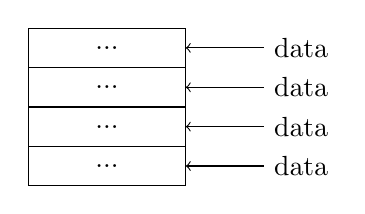
\begin{tikzpicture}
        % Draw the stack rectangles
        \draw (0,0) rectangle (2,0.5) node[pos=.5] {...};
        \draw (0,0.5) rectangle (2,1) node[pos=.5] {...};
        \draw (0,1) rectangle (2,1.5) node[pos=.5] {...};
        \draw (0,1.5) rectangle (2,2) node[pos=.5] {...};

        % Add labels
        \draw[<-] (2,0.25) -- (3,0.25) node[right] {data};
        \draw[<-] (2,0.75) -- (3,0.75) node[right] {data};
        \draw[<-] (2,1.25) -- (3,1.25) node[right] {data};
        \draw[<-] (2,1.75) -- (3,1.75) node[right] {data};
    \end{tikzpicture}
    \end{center}
    \begin{itemize}
        \item \textbf{General Concept:} The stack is a region of memory that stores data in a Last In, First Out (LIFO) manner. It is used by programs to manage function calls, local variables, and control flow.
        \item \textbf{Fixed Size:} The size of the stack is typically determined at the start of the program and is limited. Exceeding this limit can result in a stack overflow.
    \end{itemize}
    \bigbreak \noindent 
    \subsubsection{The Call Stack}
    \bigbreak \noindent 
    \begin{itemize}
        \item \textbf{Specific Use:} The term "call stack" refers more specifically to the role of the stack in storing information about the active subroutines or functions of a program. This includes return addresses, parameters passed to functions, and local variables.
        \item \textbf{Function Call Management:} Each time a function is called, a new frame (or record) is pushed onto the call stack, containing all the necessary information for that function call. When the function returns, its frame is popped off the stack.
    \end{itemize}

    \bigbreak \noindent 
    \subsection{How Many Stacks are There Per Program?}
    \bigbreak \noindent 
    in a typical C++ program (and in most conventional programming languages), there is only one stack per thread of execution. This stack is used for various purposes during the execution of your program:
    \bigbreak \noindent 
    If your C++ program is multi-threaded, each thread will have its own stack. This is because each thread has its own execution context, including function calls and local variables.

    \pagebreak 
    \subsection{Stack Memory Management}
    \bigbreak \noindent 
    Memory on the stack is automatically managed. When a function exits, all of its stack-allocated memory is reclaimed, and the stack pointer is moved back to the beginning of that memory.

    \subsection{Stack Overflow}
    \bigbreak \noindent 
    \begin{concept}
        A stack overflow is a programming error that occurs when a program uses more stack memory than is allocated to it. This typically happens in one of two scenarios:
        \begin{itemize}
            \item \textbf{Deep or Infinite Recursion:} The most common cause of a stack overflow is excessively deep or infinite recursion in a program. Each function call in most programming languages uses a bit of stack space for things like return addresses, function parameters, and local variables. In recursive functions, every recursive call adds another layer to the call stack. If the recursion is too deep or infinite (i.e., lacks a proper base case or termination condition), it can exhaust the stack memory.
            \item \textbf{Excessive Stack Allocation:} Another less common cause is allocating too much memory on the stack, such as creating very large local variables (like big arrays) inside a function. Since the stack space is limited, large allocations can fill up the stack quickly.
        \end{itemize}
    \end{concept}

    \bigbreak \noindent 
    \subsection{What Lives on The Stack?}
    \bigbreak \noindent 
    \begin{itemize}
        \item \textbf{Local Variables:} Variables declared inside a function or block (including primitive types, objects, and arrays) are allocated on the stack. Their scope and lifetime are limited to the block in which they are declared.
        \item \textbf{Function Parameters:} When a function is called, its parameters are pushed onto the stack. This includes both primitives and objects (the latter are usually passed by reference or pointer to avoid the cost of copying).
        \item \textbf{Return Addresses:} When a function is called, the address to return to at the end of the function execution is stored on the stack.
        \item \textbf{Function Call Bookkeeping:} Information such as the previous frame pointer and other housekeeping data for function calls are stored on the stack.
        \item \textbf{Temporary Objects:} Temporary objects created during expression evaluation are stored on the stack.
        \item \textbf{Non-static Local Constants:} Similar to local variables, local constants declared within a function are also stored on the stack.
        \item \textbf{Local References:} References to objects or variables that are declared within a function. However, it's important to note that while the reference itself is on the stack, the object it refers to could be anywhere (stack, heap, or global/static memory).
    \end{itemize}

    \bigbreak \noindent 
    \nt{local variables within a function are allocated on the stack, and this allocation happens each time the function is called.} 

    \pagebreak 
    \subsection{The Heap}
    \bigbreak \noindent 
    \begin{concept}
        Refers to a region of a program's memory used for dynamic memory allocation, where variables are allocated and deallocated on demand at runtime. 
    \end{concept}
    \bigbreak \noindent 
    \subsubsection{Characteristics of the Heap}
    \begin{itemize}
        \item \textbf{Dynamic Memory Allocation:} Unlike the stack, where memory is managed automatically, memory on the heap must be explicitly allocated and deallocated by the programmer. This is typically done using functions like malloc, calloc, and free in C, or new and delete in C++.
        \item \textbf{Lifetime of Memory:} Memory allocated on the heap remains allocated until it is explicitly freed, regardless of the scope where it was allocated. This allows for the creation of variables and data structures that persist beyond the scope in which they were created.
        \item \textbf{No Size Limitation:} While the stack is limited in size (decided at the start of the program), the heap can potentially use all available memory. However, using too much heap memory can lead to a condition known as "heap exhaustion" or "out of memory."
        \item \textbf{Non-contiguous Memory Allocation:} Unlike the stack, which grows and shrinks in a well-defined order, heap memory is scattered and fragmented. When you allocate memory on the heap, it can be placed anywhere in the heap's space.
        \item \textbf{Performance Considerations:} Allocating and deallocating memory on the heap is generally slower than using the stack due to the additional work required to manage free memory and possible fragmentation.
        \item \textbf{Manual Management:} Proper management of the heap is crucial. Failure to deallocate memory that is no longer needed leads to memory leaks, while accessing memory that has been deallocated leads to undefined behavior, often resulting in segmentation faults or crashes.
    \end{itemize}

    \bigbreak \noindent 
    \subsubsection{Usage}
    \begin{itemize}
        \item \textbf{Large Objects or Arrays:} The heap is often used for large data structures or arrays whose size might be too large for the stack.
        \item \textbf{Persistent Data:} When data needs to persist beyond the scope of its creation, heap allocation is used.
        \item \textbf{Dynamic Data Structures:} Data structures that grow or shrink dynamically, like linked lists, trees, and graphs, are typically allocated on the heap.
    \end{itemize}

    \pagebreak 
    \subsubsection{Heap Allocatinos in Function Bodys}
    \bigbreak \noindent 
    When you allocate memory on the heap within a function body and the allocated memory needs to outlive the pointer that points to it, you must ensure that this memory is managed correctly to avoid memory leaks and dangling pointers. Here are several strategies to handle such situations:
    \bigbreak \noindent 
    \textbf{Return the Pointer}
    \bigbreak \noindent 
    You can return the heap-allocated pointer to the caller of the function, thereby transferring the responsibility of memory management to the caller.

    \bigbreak \noindent 
    \textbf{Use Smart Pointers}
    \bigbreak \noindent 
    In C++, smart pointers (like std::unique\_ptr or std::shared\_ptr) can manage heap allocations automatically. These pointers automatically deallocate the memory when they go out of scope.

    \bigbreak \noindent 
    \textbf{Global or Static Variables}
    \bigbreak \noindent 
    In some cases (though generally less recommended due to potential issues with global state), you might assign the heap-allocated memory to a global or static variable.

    \bigbreak \noindent 
    \subsection{The Code Segment (Text Segment)}
    \bigbreak \noindent 
    \begin{itemize}
        \item The \textbf{Code Segment}, also known as the \textbf{Text Segment}, is an area of a computer program's memory where executable code is stored. This includes the compiled machine code of your program, including functions, methods, and class definitions.
        \item The Code Segment is read-only and is meant to prevent a program from accidentally modifying its instructions, ensuring the integrity of the executable code.
    \end{itemize}

    \bigbreak \noindent 
    \subsection{The Data Segment}
    \bigbreak \noindent 
    This is the part of a program's memory that holds global and static variables. The data segment is typically divided into two parts:
    \bigbreak \noindent 
    \subsubsection{Initialized Data Segment}
    \bigbreak \noindent 
    Also known as the ".data" section, this part stores global and static variables that are explicitly initialized by the programmer.
    
    \bigbreak \noindent 
    \subsubsection{Uninitialized Data Segment}
    \bigbreak \noindent 
    Also known as the "BSS" (Block Started by Symbol) section, this part stores uninitialized global and static variables. In many systems, the memory for these variables is initialized to zero by the operating system when the program starts.

    \pagebreak 
    \unsect{More on Dynamic Memory Allocation}
    \bigbreak \noindent 
    \subsection{Before we Begin: Memory Leaks}
    \bigbreak \noindent 
    \begin{concept}
    Memory leaks in programming, particularly in languages like C and C++, refer to a situation where a program fails to release memory that it has allocated. This can lead to a gradual reduction in the available memory for the program and the system, potentially causing performance degradation and even system crashes in severe cases.

    \end{concept}
    \bigbreak \noindent 
    \subsubsection{How Memory Leaks Occur}
    \begin{itemize}
        \item \textbf{Dynamically Allocated Memory Not Freed:} The most common cause of memory leaks is when a program allocates memory on the heap (using malloc, calloc, new, etc.) but does not properly release it using free or delete.
        \item \textbf{Dangling Pointers:} After freeing allocated memory, any pointers that still reference that memory become dangling pointers. If a program loses track of these pointers without freeing the associated memory first, it leads to a leak.
        \item \textbf{Repeated Allocations Without Release:} Continuously allocating new memory (e.g., within a loop) without releasing previous allocations can quickly exhaust available memory.
        \item \textbf{Data Structures Gone Wrong:} Incorrect management of dynamic data structures like linked lists, trees, or graphs can lead to parts of the structure becoming unreachable, with the memory still allocated.
    \end{itemize}
    
    \bigbreak \noindent 
    \subsection{Malloc}
    \bigbreak \noindent 
    \begin{concept}
        malloc is a function used in the C programming language (and also available in C++) for dynamic memory allocation. The name malloc stands for "memory allocation". It is used to allocate a block of memory of a specified size at runtime and returns a pointer to the beginning of this block. Here are the key aspects of malloc:
    \end{concept}
    \bigbreak \noindent 
    \subsubsection{Signature}
    \bigbreak \noindent 
    \begin{cppcode}
    void* malloc(size_t size);
    \end{cppcode}
    \bigbreak \noindent 
    Here, size is the number of bytes to allocate, and malloc returns a void* pointer to the allocated memory. This pointer can then be cast to any desired type.
    \bigbreak \noindent 
    \subsubsection{Example}
    \begin{cppcode}
    int arr[3] = {1,2,3};
    int* ptr = (int*) malloc(sizeof(int) * 4);
    // memcpy(ptr, arr, sizeof(arr));

    if (ptr == NULL) { cout << "malloc call failed to allocate memory";
    } else {
        // Unpredictable values
        for (int i=0; i<3; ++i)  {
            cout << ptr[i] << " ";
        }
    }
    free(ptr);
    ptr = nullptr;
    cout << endl;
    \end{cppcode}
    \bigbreak \noindent 
    In this example, malloc is used to allocate memory sufficient for an array of 4 integers. The returned void* pointer is cast to int*.

    \bigbreak \noindent 
    \subsubsection{Characteristics}
    \bigbreak \noindent 
    \begin{itemize}
        \item \textbf{Uninitialized Memory:} The memory block allocated by malloc is not initialized. The contents of the newly allocated block are indeterminate and may contain garbage values.
        \item \textbf{Return Value:} If the allocation is successful, malloc returns a pointer to the allocated memory. If the allocation fails (for example, due to insufficient memory), it returns NULL.
        \item \textbf{Dynamic Allocation:} Memory allocated by malloc is allocated on the heap, and its lifetime is managed manually. It remains allocated until it's explicitly freed using free(), even after the function that allocated it returns.
        \item \textbf{Size Calculation:} It's important to correctly calculate the size of memory needed, typically using the sizeof operator, to avoid under-allocating or over-allocating memory.
    \end{itemize}
    \bigbreak \noindent 
    \subsubsection{Considerations}
    \begin{itemize}
        \item \textbf{Memory Leaks:} If the memory allocated by malloc is not freed using free(), it leads to memory leaks, a common issue in long-running programs.
        \item \textbf{Error Checking:} Always check the return value of malloc to ensure that the memory allocation was successful before using the allocated memory.
        \item \textbf{C++ Alternatives:} In C++, it's recommended to use new/delete instead of malloc/free for memory allocation and deallocation. This is because new/delete also call constructors and destructors of objects, respectively, which malloc and free do not.
    \end{itemize}

    \pagebreak 
    \subsection{Calloc}
    \bigbreak \noindent 
    \begin{concept}
        Calloc Stands for "contiguous allocation" and is used to allocate memory dynamically for an array of elements, initializing all bytes to zero.
    \end{concept}
    \bigbreak \noindent 
    \subsubsection{Signature}
    \bigbreak \noindent 
    \begin{cppcode}
        void* calloc(size_t numElements, size_t sizeOfElement);
    \end{cppcode}
    \bigbreak \noindent 
    \subsubsection{Example}
    \bigbreak \noindent 
    \begin{cppcode}
    int* ptr = (int*) calloc(3, sizeof(int));

    // Ouput: 0 0 0
    if (ptr == nullptr) { cout << "Calloc call failed";
    } else {
        for (int i=0; i<3; ++i)  {
            cout << ptr[i] << " ";
        }
    }
    free(ptr);
    ptr = nullptr;
    \end{cppcode}

    \bigbreak \noindent 
    The function returns a pointer to the allocated memory, or \textbf{NULL} if the allocation fails.
    \bigbreak \noindent 
    \subsubsection{Differences from malloc}
    \bigbreak \noindent 
    \begin{itemize}
        \item \textbf{calloc} initializes the allocated memory to zero, while malloc does not initialize the memory.
        \item \textbf{calloc} takes two arguments (number of elements and size of each element), whereas malloc takes only one argument (total size in bytes).
    \end{itemize}

    \bigbreak \noindent 
    \subsection{Realloc}
    \bigbreak \noindent 
    \begin{concept}
       The purpose of realloc is to resize a previously allocated memory block. It's typically used when you need to either increase or decrease the size of a memory block that was previously allocated with malloc, calloc, or a previous call to realloc. 
    \end{concept}
    \bigbreak \noindent 
    \subsubsection{Signature}
    \bigbreak \noindent 
    \begin{cppcode}
    void* realloc(void* ptr, size_t newSize);
    \end{cppcode}
    \bigbreak \noindent 
    Where 
    \bigbreak \noindent 
    \begin{itemize}
        \item \textbf{ptr:} Pointer to the memory block previously allocated. If this is nullptr, realloc behaves like malloc.
        \item \textbf{newSize:} The new size for the memory block in bytes.
    \end{itemize}

    \bigbreak \noindent 
    \subsubsection{Example}
    \bigbreak \noindent 
    \begin{cppcode}
    int* ptr = (int*) calloc(4, sizeof(int));

    if (ptr != nullptr ) {
        int* newptr = static_cast<int*>(realloc(ptr, sizeof(int) * 10));
        if (newptr != nullptr) {
            ptr = newptr;
        } 
    }

    free(ptr);
    ptr = nullptr;
    \end{cppcode}
    

    \bigbreak \noindent 
    \subsection{Free}
    \bigbreak \noindent 
    \begin{concept}
        \textbf{free()} is a function used in both C and C++ for deallocating memory that was previously allocated by a call to \textbf{malloc()}, \textbf{calloc()}, or \textbf{realloc()}. It is part of the C standard library, and its functionality is the same in both C and C++ when dealing with memory allocated by these C standard library functions. 
    \end{concept}
    \bigbreak \noindent 
    \subsubsection{Signature}
    \bigbreak \noindent 
    \begin{cppcode}
    void free(void* ptr);
    \end{cppcode}
    \bigbreak \noindent 
    Where
    \begin{itemize}
        \item \textbf{ptr:} A pointer to the memory block to be freed. This pointer must have been returned by a previous call to malloc(), calloc(), or realloc(). If ptr is a null pointer (nullptr in C++, NULL in C), no action occurs.
    \end{itemize}
    

    \bigbreak \noindent 
    \subsection{New}
    \bigbreak \noindent 
    \begin{concept}
        \textbf{new} is a C++ operator used for dynamic memory allocation. Unlike malloc in C which only allocates memory, new not only allocates memory but also initializes the object. It's a fundamental part of C++'s object-oriented features, offering several advantages and features:
    \end{concept}
    \bigbreak \noindent 
    \subsubsection{Syntax}
    \bigbreak \noindent 
    \begin{cppcode}
    TypeName* variable = new TypeName;
    \end{cppcode}
    \bigbreak \noindent 
    \subsubsection{Array allocation}
    \bigbreak \noindent 
    \begin{cppcode}
    int* myArray = new int[10]; // Allocates an array of 10 integers
    \end{cppcode}
    \bigbreak \noindent 
    \subsubsection{Custom Constructor Parameters}
    \bigbreak \noindent 
    \begin{cppcode}
    MyClass* myObject = new MyClass(5);
    \end{cppcode}
    \bigbreak \noindent 
    \subsubsection{Exception Handling (std::nothrow)}
    \bigbreak \noindent 
    If new fails to allocate memory (typically due to memory exhaustion), it throws a std::bad\_alloc exception, unless it's the nothrow variant:
    \bigbreak \noindent 
    \begin{cppcode}
    int* myArray = new (std::nothrow) int[1000000000];
    if (!myArray) {
        // Handle allocation failure
    }
    \end{cppcode}

    \pagebreak 
    \subsubsection{Placement New}
    \bigbreak \noindent 
    \begin{cppcode}
    #include <new> // For placement new
    char buffer[sizeof(MyClass)];
    MyClass* myObject = new (buffer) MyClass;
    \end{cppcode}
    \bigbreak \noindent 
    \nt{A char array is often used as a buffer for placement new due to a few key reasons:
        \begin{itemize}
            \item \textbf{General Compatibility:} char types are guaranteed to have the least strict alignment requirements of all types. This means that a char array is suitably aligned for any data type.
            \item \textbf{Avoiding Undefined Behavior:} More strictly aligned types (like int or double) may not be correctly aligned in a buffer of a less strictly aligned type. But you can place any object in a char buffer without violating alignment requirements, which is crucial to avoid undefined behavior.
            \item \textbf{Precise Size Specification:} A char in C++ is exactly one byte in size. Using a char array allows you to allocate a buffer with a very precise size, equal to the number of bytes needed.
            \item \textbf{Flexibility for Different Types:} This precision and flexibility make char arrays a common choice for memory buffers that might need to store various types of data.
        \end{itemize}
        Its important to know that the object will not be on the heap.
    }

    \bigbreak \noindent 
    \subsection{Delete}
    \bigbreak \noindent 
    \begin{concept}
        The delete operator in C++ is used to deallocate memory that was previously allocated by the new operator. It plays a crucial role in memory management and prevents memory leaks by ensuring that dynamically allocated memory is properly released back to the system. Here's a closer look at how delete works:
    \end{concept}
    \bigbreak \noindent 
    \subsubsection{Syntax}
    \bigbreak \noindent 
    \begin{cppcode}
    int* ptr = new int; // Allocation
    delete ptr; // Deallocation
    delete[] ptr; // If ptr was an array
    \end{cppcode}
    \nt{If delete is called on an object, the destructor for the object is automatically called. Furthermore, the memory will be released back to the system.}
    

    \bigbreak \noindent 
    \subsection{Dangling Pointers}
    \bigbreak \noindent 
    \begin{concept}
        After freeing a memory block, the pointer variable itself is not changed. It still points to the same memory address, but this address is no longer valid. Such a pointer is known as a "dangling pointer". To prevent accidental use of dangling pointers, it's a good practice to set the pointer to nullptr immediately after freeing it.
    \end{concept}

    \pagebreak 
    \subsection{Overloading new and delete}
    \bigbreak \noindent 
    \begin{concept}
        Overloading the new and delete operators in C++ allows you to provide custom behavior for memory allocation and deallocation. This can be useful for debugging memory usage, implementing custom memory pools, or tracking memory allocation statistics. Here's a basic example to illustrate how you might overload these operators for a specific class.
    \end{concept}
    \bigbreak \noindent 
    \begin{cppcode}
class MyClass {
public:
    // Overload the "new" operator for MyClass
    static void* operator new(size_t size) {
        std::cout << "Allocating " << size << " bytes for MyClass" << std::endl;
        void* ptr = std::malloc(size);
        if (!ptr) throw std::bad_alloc(); // Handle allocation failure
        return ptr;
    }

    // Overload the "delete" operator for MyClass
    static void operator delete(void* ptr) {
        std::cout << "Deallocating memory for MyClass" << std::endl;
        std::free(ptr);
    }
};

int main() {
    MyClass* obj = new MyClass; // Calls overloaded "new"

    delete obj; // Calls overloaded "delete"
    return 0;
}
    \end{cppcode}
    \bigbreak \noindent 
    \subsubsection{Why static?}
    \begin{itemize}
        \item \textbf{Class-Level Operation:} Although new is used for creating instances, the memory allocation part of its job is independent of any specific instance of the class. It's about preparing a space where an instance will be created.
        \item \textbf{No Instance Context Needed:} At the point where new is doing its work (allocating memory), there is no instance of the object yet. Hence, this operation cannot be associated with an instance — it's associated with the class itself.
        \item \textbf{Static Nature:} This is why new is a static member function when overloaded in a class. It operates in the context of the class, not individual instances. It's about providing a service (memory allocation) that is a prerequisite for instance creation.
    \end{itemize}
    \pagebreak 
    \subsubsection{The size\_t parameter in the new overload}
    \bigbreak \noindent 
     The size parameter in the new operator represents the size of the object being created. This is automatically provided by the C++ runtime.

     \bigbreak \noindent 
    \subsection{Getting the size of dynamically allocated memory?}
    \bigbreak \noindent 
    \begin{concept}
        In C and C++, there is no direct way to retrieve the size of a dynamically allocated memory block from the pointer itself. The sizeof operator, when used on a pointer, will always return the size of the pointer type, not the size of the memory block it points to. 
        \bigbreak \noindent 
        When you allocate memory dynamically, you're responsible for keeping track of its size. There are a few common approaches to handle this:
    \end{concept}


    \bigbreak \noindent 
    \subsection{Mixing Memory Management Mechanism}
    \bigbreak \noindent 
    \begin{concept}
        You should not use the delete operator with memory allocated by malloc, calloc, or realloc in C++. Similarly, you should not use free with memory allocated by new. This is because new and delete are C++ operators that not only manage memory but also call constructors and destructors of objects, while malloc, calloc, and realloc are C library functions that merely allocate or deallocate memory without any regard for constructors or destructors.
        \begin{itemize}
            \item In C and C++, when you allocate memory using malloc, calloc, or realloc, you should deallocate it using free. These functions are part of the C standard library and are focused solely on memory allocation and deallocation.
            \item In C++, when you allocate memory using new, you should deallocate it using delete. Similarly, for arrays allocated with new[], use delete[] to deallocate. The new and delete operators handle both memory management and object lifecycle (calling constructors and destructors).
        \end{itemize}
    \end{concept}
    \bigbreak \noindent 
    \subsubsection{Why Mixing Them is Bad}
    \begin{itemize}
        \item \textbf{Different Memory Management Mechanisms:} new/delete and malloc/free use potentially different memory management mechanisms. Using delete on a malloc-allocated block (or free on a new-allocated block) can lead to undefined behavior, such as memory corruption or program crashes.
        \item \textbf{Constructors and Destructors:} new and delete manage object construction and destruction, which malloc and free do not. Using malloc with non-trivially constructible types will not call constructors, and using delete on such memory will not call the correct destructors.
    \end{itemize}

    \bigbreak \noindent 
    \subsection{Should you be using malloc, calloc, realloc, or free in C++?}
    \bigbreak \noindent 
    \begin{concept}
        \textbf{NO:} Using \textbf{new and delete} in C++ is generally preferred over C-style functions like malloc(), calloc(), realloc(), and free() due to several reasons, primarily related to C++'s object-oriented features, type safety, and abstraction level:
    \end{concept}
    \bigbreak \noindent 
    \subsubsection{Constructor and Destructor Calls}
    \begin{itemize}
        \item \textbf{C++ Objects Initialization:} new automatically calls the constructor of the object, initializing it properly. Similarly, delete calls the destructor. This ensures that objects are both created and destroyed correctly, following C++'s principles of object-oriented programming.
        \item \textbf{No Constructor/Destructor with C Functions:} malloc and calloc merely allocate memory without initializing the object. They cannot be used for objects that require constructors. Similarly, free does not call destructors, which can lead to resource leaks (like not releasing file handles, network connections, etc.) if an object manages such resources.
    \end{itemize}

    \bigbreak \noindent 
    \subsubsection{Type Safety}
    \begin{itemize}
        \item \textbf{Automatic Type Casting:} new returns a pointer of the correct type, eliminating the need for explicit casting as required with malloc or calloc.
        \item \textbf{Error Proneness of Explicit Casting:} The casting required with malloc can lead to errors if the wrong type is cast, potentially leading to undefined behavior.
    \end{itemize}

    \bigbreak \noindent 
    \subsubsection{Exception Handling}
    \begin{itemize}
        \item \textbf{Throwing Exceptions on Failure:} new throws an exception (std::bad\_alloc) if it fails to allocate memory, allowing the use of C++ exception handling to manage memory allocation errors.
        \item \textbf{No Exception Handling with C Functions:} malloc and calloc return nullptr on failure, requiring manual error checking after each allocation.
    \end{itemize}

    \pagebreak 
    \unsect{Other Casting Operators}
    \bigbreak \noindent 

    \subsection{dynamic\_cast}
    \bigbreak \noindent 
    \begin{concept}
        The \textbf{dynamic\_cast} in C++ is a type of casting operator used primarily for safe downcasting at runtime. Downcasting refers to the process of converting a pointer or reference from a base class to a derived class. This is important in the context of polymorphism and inheritance in C++. Here's a detailed explanation:
    \end{concept}
    \bigbreak \noindent 
    \subsubsection{Purpose}
    \begin{itemize}
        \item \textbf{Safe Downcasting:} dynamic\_cast is used to safely convert pointers and references to classes up, down, or sideways along the inheritance hierarchy.
        \item \textbf{Runtime Type Checking:} Unlike other casts in C++, dynamic\_cast performs a runtime check to ensure the validity of the cast. If the cast is not possible, it either returns nullptr (for pointers) or throws a std::bad\_cast exception (for references).
    \end{itemize}
    \bigbreak \noindent 
    \subsubsection{Syntax}
    \bigbreak \noindent 
    \begin{cppcode}
    Derived *d = dynamic_cast<Derived*>(base_ptr);
    Derived &d = dynamic_cast<Derived&>(base_ref);
   \end{cppcode}

   \bigbreak \noindent 
   \subsubsection{Requirements}
   \begin{itemize}
        \item \textbf{Polymorphic Base Class:} For dynamic\_cast to work, the class from which you are casting must be polymorphic, which means it should have at least one virtual function. This is required because dynamic\_cast relies on runtime type information (RTTI) to check the validity of the cast.
        \item \textbf{Public Inheritance:} dynamic\_cast can only be used with classes that are publicly inherited. It doesn’t work with private or protected inheritance.
   \end{itemize}

   \bigbreak \noindent 
   \subsubsection{Example}
   \bigbreak \noindent 
   \begin{cppcode}
class Base { virtual void dummy() {} };
class Derived: public Base { /* ... */ };

Base *base_ptr = new Derived;
Derived *derived_ptr = dynamic_cast<Derived*>(base_ptr);

if (derived_ptr) {
    // The cast is successful
}
   \end{cppcode}
    

    \bigbreak \noindent 
    \subsection{const\_cast}
    \bigbreak \noindent 
    \begin{concept}
        The \textbf{const\_cast} in C++ is a type casting operator used to explicitly override constness or volatility of a variable. It allows you to modify a non-const variable which is accessed through a pointer or reference to const. It's important to understand how and when to use it correctly, as misuse can lead to undefined behavior.
        \bigbreak \noindent 
        \textbf{const\_cast} is exclusively used to add or remove the const (or volatile) qualifier from a pointer or reference. It's typically used to cast away the constness of a variable, allowing a const variable to be modified.
    \end{concept}
    \subsubsection{Removing const}
    \bigbreak \noindent 
    \begin{cppcode}
    int nonConstVar = 30;
    const int* ptrToConst = &nonConstVar; // Pointer to const
    int* modifiablePtr = const_cast<int*>(ptrToConst); // Casting away constness
    *modifiablePtr = 40; // Safe, because the original variable is non-const

    cout << nonConstVar << endl; // Will print 40
    \end{cppcode}

    \bigbreak \noindent 
    \subsubsection{Adding const}
    \bigbreak \noindent 
    \begin{cppcode}
    int a = 15;
    int* b = &a;
    const int* c = const_cast<const int*>(b); // Cannot use c to modify a
    \end{cppcode}
    \bigbreak \noindent 
    \nt{While const\_cast can be used to add constness, it's more commonly used to remove constness in scenarios where you're interfacing with code that hasn't been written with const correctness in mind but you know it won't modify the data.
        \bigbreak \noindent 
        the direct assignment is simpler, clearer, and more idiomatic in C++. const\_cast should be reserved for scenarios where you need to remove constness, or when dealing with APIs or legacy code that requires it.
    }

    \bigbreak \noindent 
    \subsubsection{Use cases}
    \begin{itemize}
        \item \textbf{Interfacing with Non-const Functions:} If you have a function that doesn't modify its parameters but hasn't used const in its parameters, you may need to use const\_cast to pass const variables to it.
       \item \textbf{Legacy Code:} In older codebases that don't use const correctly, const\_cast can be a workaround to make the code compile without modifying a large codebase.
    \end{itemize}

    \bigbreak \noindent 
    \subsubsection{Important Points}
    \begin{itemize}
        \item \textbf{Undefined Behavior:} Modifying a variable that is originally declared as const leads to undefined behavior. const\_cast should be used only when you are certain that the actual object isn't const.
        \item \textbf{Const Safety:} It should be used sparingly and only when necessary, as it breaks the promise of constness, which is a fundamental aspect of C++ for ensuring safety and predictability of the code.
        \item \textbf{No Actual Conversion:} const\_cast does not perform a real conversion. It only adds or removes the const/volatile qualifier.
    \end{itemize}

    \bigbreak \noindent 
    \subsubsection{Example}
    \bigbreak \noindent 
    \begin{cppcode}
void printWithoutConst(const int* ptr) {
    int* modifiablePtr = const_cast<int*>(ptr);
    *modifiablePtr = 5; // Only safe if 'ptr' wasn't pointing to an originally const object
    std::cout << *ptr << std::endl;
}

int main() {
    int value = 10;
    printWithoutConst(&value); // Safe, since 'value' is not a const
    return 0;
}
    \end{cppcode}

    \bigbreak \noindent 
    \subsubsection{When is it unsafe to use}
    \bigbreak \noindent 
    We should not use a const\_cast to modify objects that were declared as const, as this will lead to undefined behavior

    \bigbreak \noindent 
    \subsubsection{The volatile keyword}
    \bigbreak \noindent 
    \begin{concept}
        The \textbf{volatile} keyword in C++ is a type qualifier used to indicate that a variable's value may change unexpectedly. It is typically used in scenarios involving hardware access, low-level programming, or handling a variable modified by an external event such as an interrupt.
    \end{concept}
    \bigbreak \noindent 
    \subsubsection{Purpose}
    \begin{itemize}
        \item \textbf{Preventing Compiler Optimizations:} Normally, compilers optimize the code by caching variables in registers and removing redundant reads and writes. By declaring a variable as volatile, you instruct the compiler that the variable can change at any time, so it should not optimize the access to this variable. Every read and write to a volatile variable is a direct read and write from and to the memory location of the variable.
        \item \textbf{Use in Embedded Systems and Hardware Programming:} volatile is commonly used in embedded systems, where variables might be modified by hardware events outside the control of the program. For instance, a memory-mapped hardware register's state might change independently, and volatile ensures that the program always reads the current state.
    \end{itemize}
    

    \bigbreak \noindent 
    \subsection{reinterpret\_cast}
    \bigbreak \noindent 
    \begin{concept}
        \textbf{reinterpret\_cast} in C++ is a type of casting operator that allows you to convert any pointer type to any other pointer type, including unrelated types. It also allows casting from pointer to an integer type and vice versa. This cast performs no runtime checks, which makes it a powerful but potentially dangerous tool if used incorrectly.
    \end{concept}
    \bigbreak \noindent 
    \subsubsection{Key Characteristics}
    \begin{itemize}
        \item \textbf{Low-Level Cast:} reinterpret\_cast is used for low-level reinterpreting of the bit patterns of the data. It doesn't perform any kind of compatibility check or conversion.
        \item \textbf{Pointer Conversions:} It's typically used to convert pointers of one type to another, regardless of whether the types are related.
        \item \textbf{No Guarantee on Data Preservation:} The result of the conversion might not point to a meaningful or valid object of the target type. It depends entirely on the specific use case and understanding of the memory layout
    \end{itemize}
    \bigbreak \noindent 
    \subsubsection{Syntax}
    \bigbreak \noindent 
    \begin{cppcode}
    TargetType* ptr = reinterpret_cast<TargetType*>(sourcePointer);
    \end{cppcode}
    \bigbreak \noindent 
    \subsubsection{Example}
    \bigbreak \noindent 
    \begin{cppcode}
    char* charPtr = new char[10]; // Pointer to a memory block
    int* intPtr = reinterpret_cast<int*>(charPtr); // Reinterpret as an int pointer
    \end{cppcode}
    \bigbreak \noindent 
    In this example, charPtr is a pointer to a character array, and intPtr is the same memory block reinterpreted as a pointer to an integer. Note that the actual content of memory is not changed; only the type through which the memory is accessed is changed.

    \bigbreak \noindent 
    \subsubsection{Considerations}
    \begin{itemize}
        \item \textbf{Potential for Undefined Behavior:} Because reinterpret\_cast does not check the compatibility of the types involved, using it incorrectly can easily lead to undefined behavior.
        \item \textbf{Use Sparingly:} Given its power and potential for misuse, it should be used sparingly and only when you are certain about the memory layout and the requirements of your application.
        \item \textbf{Alternative Solutions:} Before using reinterpret\_cast, consider if the same goal can be achieved using safer casts like static\_cast or dynamic\_cast. Use reinterpret\_cast only when other casts are not suitable for your needs.
    \end{itemize}

    \pagebreak 
    \unsect{Namespaces}
    \bigbreak \noindent 
    \begin{concept}
        Namespaces in C++ are a feature used to organize code into discrete sections, helping to prevent name conflicts in larger projects. 
        \bigbreak \noindent 
        Namespaces are primarily used to avoid name collisions which can occur when your code base includes multiple libraries. For instance, two different libraries might both define a class or function named Logger. Without namespaces, these would clash, potentially causing errors.
    \end{concept}

    \bigbreak \noindent 
    \subsection{Syntax}
    \bigbreak \noindent 
    \begin{cppcode}
    namespace MyNamespace {
        void myFunction() {
            // Function implementation
        }
    }
    \end{cppcode}

    \bigbreak \noindent 
    \subsection{Using Namespaces}
    \bigbreak \noindent 
    \begin{itemize}
        \item \textbf{Accessing Elements:} To use myFunction defined in MyNamespace, you would call it like this: MyNamespace::myFunction().
        \item \textbf{Using Directive:} If you don't want to prefix every use of elements from a namespace, you can use the using directive:
            \bigbreak \noindent 
            \begin{cppcode}
            using namespace MyNamespace;
            \end{cppcode}
    \end{itemize}

    \bigbreak \noindent 
    \subsection{Nested Namespaces} 
    \bigbreak \noindent 
    Namespaces can be nested within each other, allowing for further organization. 
    \bigbreak \noindent 
    \begin{cppcode}
    namespace Outer {
        namespace Inner {
            int x;
        }
    }
    cout << outer::inner::x  << endl;
    \end{cppcode}

    \bigbreak \noindent 
    \subsection{Anonymous Namespaces}
    \bigbreak \noindent 
    These are unnamed namespaces that are unique to the translation unit they are defined in. They are useful for declaring objects or functions that should only be accessible within a single file. 
    \bigbreak \noindent 
    \begin{cppcode}
    namespace {
        int x;
    }
    cout << x; 
    \end{cppcode}

    \pagebreak 
    \unsect{Exceptions}
    \bigbreak \noindent 
    \begin{concept}
        Exception handling in programming is a mechanism to handle runtime errors in a controlled manner. In languages like C++, Java, and Python, it allows a program to continue executing even if an error occurs, rather than crashing immediately. 
    \end{concept}
    \bigbreak \noindent 
    \subsection{Concepts}
    \begin{itemize}
        \item \textbf{Exception:} An exception is an event, typically an error, that disrupts the normal flow of the program. It could be caused by factors like invalid input, hardware failure, or resource exhaustion.
        \item \textbf{Try Block:} This is where you place code that might throw an exception. The idea is to "try" to execute this code, but it might lead to an exception.
        \item \textbf{Catch Block:} If an exception is thrown in the try block, the catch block is executed. This block "catches" the exception and contains code to handle it. In many languages, you can have multiple catch blocks to handle different types of exceptions.
        \item \textbf{Finally Block (in some languages):} This block is executed after the try and catch blocks, regardless of whether an exception was thrown or caught. It's typically used for cleanup activities.
        \item \textbf{Throwing Exceptions:} In many languages, you can throw an exception using the throw keyword. You can throw either built-in exception types or custom ones.
    \end{itemize}

    \bigbreak \noindent 
    \subsection{Syntax}
    \bigbreak \noindent 
    \begin{cppcode}
        try {
            // ... code to try
        } catch ( [ some exception ] ) {
            // ... code to run if an exception is caught
        } catch ( [ some exception ] ) {
            // ... we can define many catch blocks to handle different exceptions
        }
    \end{cppcode}

    \pagebreak 
    \subsection{Example}
    \bigbreak \noindent 
    \begin{cppcode}
        #include <exception> // Full exception class
        #include <stdexcept> // Child with less exceptions

        int main() {
            try {
                // Code that may throw an exception
                throw std::runtime_error("A sample error occurred");
            } catch (const std::runtime_error& e) {
                // Code to handle the exception
                std::cerr << "Caught an exception: " << e.what() << std::endl;
            }
            // The program continues here after the catch block
            return 0;
        }

    \end{cppcode}

    \bigbreak \noindent 
    \subsection{Why does catch take a const reference?}
    \bigbreak \noindent 
    The catch clause in C++ exception handling is used to capture and handle exceptions that are thrown in the associated try block. When you catch an exception as a const reference (e.g., catch (const std::exception\& e)), it's for several important reasons:
    \bigbreak \noindent 
    \subsubsection{Safety and Efficiency}
    \begin{itemize}
        \item \textbf{Avoiding Copies:} Catching by reference avoids making a copy of the exception object. If you catch by value, C++ creates a copy of the exception object, which can be inefficient, especially for large exception objects.
        \item \textbf{Preserving Polymorphism:} When you catch by reference, you maintain the polymorphic nature of exceptions. Exceptions in C++ are often used in a hierarchy (e.g., inheriting from std::exception). Catching by reference ensures that the derived class type is preserved. If you catch by value, you might slice the object, meaning that you only catch the base part of a derived object, losing the derived class information.
    \end{itemize}

    \bigbreak \noindent 
    \subsubsection{Const Correctness}
    \bigbreak \noindent 
    \begin{itemize}
        \item \textbf{Preventing Modification:} Catching as const ensures that the exception object cannot be modified inside the catch block. This is a good practice because you typically want to treat exception objects as read-only — they are meant to convey information about an error, not to be altered.
        \item \textbf{Immutable Error State:} By enforcing const-ness, you maintain the integrity of the information contained in the exception object, ensuring that the error state it represents remains unchanged.
    \end{itemize}

    \bigbreak \noindent 
    \subsection{Catching any exception}
    \bigbreak \noindent 
    \begin{cppcode}
        catch (const std::exception& e)
    \end{cppcode}

    \bigbreak \noindent 
    \subsection{cerr (standard error)}
    \bigbreak \noindent 
    \textbf{std::cerr} in C++ is one of the standard stream objects provided for performing output, specifically for error messages. It stands for "C++ Error". Like \textbf{std::cout}, which is used for general output, \textbf{std::cerr} is used to output to the standard error (stderr) stream. Here are some key points about \textbf{std::cerr}:
    \bigbreak \noindent 
    \subsubsection{Unbuffered Output}
    \begin{itemize}
        \item \textbf{std::cerr} is unbuffered. This means that output to \textbf{std::cerr} is displayed immediately without being stored in a buffer first. This is especially useful for error messages, where immediate output can be crucial for diagnosing problems, particularly if the program crashes or terminates unexpectedly.
    \end{itemize}

    \bigbreak \noindent 
    \subsection{The what() function}
    \bigbreak \noindent 
    \subsubsection{Signature}
    \bigbreak \noindent 
    The what function is a member of exception objects, and it is used to return an explanatory string.
    \begin{cppcode}
    virtual const char* what() const throw(); // Having throw() is the same as having noexcept
    virtual const char* what() const noexcept;
    \end{cppcode}

    \bigbreak \noindent 
    \subsection{What can we throw/catch?}
    \bigbreak \noindent 
    Throwing and catching errors in C++ is not limited to standard exceptions like \textbf{std::runtime\_error}. We throw whatever objects we want.
    \bigbreak \noindent 
    \begin{cppcode}
        int x = -1;
        try {
            cout << "Inside try \n";
            if (x < 0) {
                throw x;
            }
        } catch (int intToCatch ) {
            cerr << "Exception Caught \n";
        }
    \end{cppcode}
    \bigbreak \noindent 
    \nt{The reason we have \texttt{int intToCatch} in our catch block is because we want to catch integer values that may have been thrown. Since the value we are throwing is an integer, our catch block will handle it}

    \bigbreak \noindent 
    \subsection{noexcept in function signatures}
    \bigbreak \noindent 
    \begin{concept}
        The \textbf{noexcept} specifier in C++ function signatures is used to indicate that a function is guaranteed not to throw any exceptions. This specifier plays a crucial role in exception safety and can help in optimizing C++ programs. Here's a detailed explanation:
    \end{concept}

    \bigbreak \noindent 
    \subsection{Syntax and Usage}
    \bigbreak \noindent 
    \begin{cppcode}
        void myFunction() noexcept;
        void myFunction() throw(); // Does the same thing
    \end{cppcode}
    \bigbreak \noindent 
    \nt{If a noexcept function does throw an exception, the program will call std::terminate(), resulting in immediate program termination. This is a significant difference compared to functions without the noexcept specifier, where thrown exceptions can be caught by a catch block.}

    \bigbreak \noindent 
    \subsection{Benefits}
    \begin{itemize}
        \item \textbf{Optimization:} Compilers can perform optimizations on functions that are marked as noexcept because they don't need to account for the possibility of stack unwinding due to exceptions. This can lead to more efficient code, especially in performance-critical software.
        \item \textbf{Exception Safety Guarantees:} Using noexcept clearly communicates to other programmers that the function is guaranteed not to throw exceptions. This is part of writing exception-safe code, which is crucial in robust application design.
        \item \textbf{Move Operations:} In modern C++ (C++11 and later), move constructors and move assignment operators that are noexcept are more likely to be used by the standard library containers. This makes operations like resizing a std::vector more efficient since it can safely move objects rather than copy them.
    \end{itemize}

    \pagebreak 
    \subsection{OOP Approach to exceptions (Custom exception class)}
    \bigbreak \noindent 
    Consider the example\bigbreak \noindent 
    \begin{cppcode}
        class foo {
            private:
            int x;

            public:
            foo() = default;
            class bad { 
                private:
                    int value;
                public:
                    bad(int val) : value(val) {}
                    int getValue() const { return this->value; }
            };

            void set(int val) {
                if ( val >= 0 ) { this->x = val;} 
                else { throw bad(val); }
            }
        };

        int main(int argc, const char* argv[]) { 
            foo f1;

            try {
                f1.set(-5);
            } catch (const foo::bad& e) {
                std::cerr << "Error found, bad value: " << e.getValue() << endl;
            }

            return EXIT_SUCCESS; 
        }
    \end{cppcode}
    \bigbreak \noindent 
    \begin{itemize}
        \item \textbf{Custom Exception Class:} class bad {}; defines a simple custom exception class within foo. This class just defines a value member to hold the bad value and a method to retrieve it.
    \end{itemize}

    \pagebreak 
    \subsection{Unwinding the stack}
    \bigbreak \noindent 
    \begin{concept}
        Once an exception has been thrown, the program cannot jump back to the throw point.
        The function that executes a throw statement will immediately terminate. If that function was called by another function, and the exception is not caught, then the calling
        function will terminate as well. This process, known as unwinding the stack,continues
        for the entire chain of nested function calls, from the throw point, all the way back to
        the try block.
        \bigbreak \noindent 
        If an exception is thrown by the member function of a class object, then the class destructor
        is called. If statements in the try block or branching from the try block created any other
        objects, their destructors will be called as well. 
    \end{concept}

    \bigbreak \noindent 
    \subsection{More on 'new'}
    \bigbreak \noindent 
    \subsubsection{Handling bad\_alloc}
    \bigbreak \noindent 
    \begin{cppcode}
        int* ptr = nullptr;

        try {
            ptr = new int[10000000000000];
            cout << "Allocation success" << endl;
        } catch(const std::bad_alloc& e) {
        }
        std::cerr << "Allocation failed: " << e.what() << endl;
    \end{cppcode}

    \bigbreak \noindent 
    \subsubsection{nothrow}
    \bigbreak \noindent 
    The nothrow version of new is a way to instruct the operator not to throw an exception on failure, but to return a null pointer instead.
    \bigbreak \noindent 
    \begin{cppcode}
        int* ptr = nullptr;
        ptr = new(std::nothrow) int[10000000000000];

        if (ptr == nullptr) {
            cout << "Allocation Failed" << endl;
        } else {
            cout << "Allocation Success" << endl;
        }
    \end{cppcode}

    \pagebreak 
    \unsect{Templates}
    \bigbreak \noindent 
    \subsection{Function Templates}
    \bigbreak \noindent 
    \begin{concept}
        \textbf{Function templates} enable you to write a single function that can operate on different data types. The compiler generates the appropriate function based on the type of argument passed.
    \end{concept}
    \bigbreak \noindent 
    \subsubsection{Syntax}
    \bigbreak \noindent 
    \begin{cppcode}
    template<typename T>
    T name(T p1, T p2, ...) {
        // Function Body...
    }
    \end{cppcode}

    \bigbreak \noindent 
    \subsubsection{Example}
    \bigbreak \noindent 
    \begin{cppcode}
    template<typename T>
    T foo(T a, T, b) {
        return a*b;
    }
    foo(1,2) // Output: 2
    \end{cppcode}


    \pagebreak 
    \subsection{Class Templates}
    \bigbreak \noindent 
    \begin{concept}
        \textbf{Class templates} allow you to define a class to work with any data type. Like function templates, the compiler generates the necessary class based on the data type used.
    \end{concept}
    \bigbreak \noindent 
    \subsubsection{Example}
    \bigbreak \noindent 
    \begin{cppcode}
        template<typename T>
        class foo {
        private:
            T* arr;
            size_t size;
        public:
            foo() = default;

            foo(std::initializer_list<T> il) {

                size = il.size();
                arr = new T[size];

                T tmp[size];
                std::move(il.begin(), il.end(), tmp);

                memcpy(arr, tmp, sizeof(tmp));
            }

            void Print() {
                for (size_t i=0; i<size; ++i) {
                    cout << arr[i] << " ";
                }
                cout << endl;
            }

            ~foo() { delete[] arr; }


        };
        int main(int argc, const char* argv[]) {

            foo<int> f1({1,2,3});
            foo<float> f2({1.232,2.232,3.121});
            foo<char> f3({'a', 'b', 'c'});

            return EXIT_SUCCESS;
        }
    \end{cppcode}

    \pagebreak 
    \subsection{Function Template Specialization}
    \bigbreak \noindent 
    \begin{concept}
        \textbf{Template specialization} allows you to define a different implementation for a particular data type.
    \end{concept}
    \bigbreak \noindent 
    \begin{cppcode}
    template <typename T>
    T min(T x, T y) {
        return (x < y) ? x : y;
    }

    template <>
    const char* min(const char* x, const char* y) {
        return (strcmp(x, y) < 0) ? x : y;
    }
    \end{cppcode}

    \bigbreak \noindent 
    \subsection{Class/Struct Template Specialization}
    \bigbreak \noindent 
    \begin{cppcode}
    template<typename T>
    struct foo {
        T x = 20;
    };

    template<>
    struct foo<char> {
        char x = 'z';
    };
    \end{cppcode}

    \bigbreak \noindent 
    \subsection{Template Parameters}
    \bigbreak \noindent 
    \begin{concept}
        Templates can have more than one parameter, including non-type parameters.
    \end{concept}
    \bigbreak \noindent 
    \begin{cppcode}
        template <typename T, int size>
        class FixedArray {
            private:
            T arr[size];
            // implementation
        };
    \end{cppcode}

    \bigbreak \noindent 
    \subsection{Trailing return type}
    \bigbreak \noindent 
    In traditional C++, the return type of a function is declared at the beginning of the function declaration. However, C++11 introduced a new syntax that allows the return type to be specified after the parameter list, using auto at the beginning and -> Type after the parameter list.
    \bigbreak \noindent 
    \subsubsection{Syntax}
    \bigbreak \noindent 
    \begin{cppcode}
    auto functionName(parameters) -> returnType {
        // function body
    }
    \end{cppcode}

    \bigbreak \noindent 
    \subsubsection{Example}
    \bigbreak \noindent 
    \begin{cppcode}
    auto foo(int a, int b) -> int {
        return a + b;
    }
    \end{cppcode}

    \bigbreak \noindent 
    \subsection{decltype}

    \bigbreak \noindent 
    \begin{concept}
        \textbf{decltype} is a keyword in C++ introduced in C++11, which stands for "declared type". It is used to query the type of an expression without actually evaluating that expression. This can be particularly useful in template programming and type deduction, where the type of an expression might not be known until compile time.
    \end{concept}
    \bigbreak \noindent 
    \subsubsection{Syntax}
    \bigbreak \noindent 
    \begin{cppcode}
        decltype(expression) variable_name;
    \end{cppcode}
    \bigbreak \noindent 
    Here, \textbf{variable\_name} will have the same type as the type of \textbf{expression}. It's important to note that \textbf{expression} is not evaluated; \textbf{decltype} only deduces its type.
    \bigbreak \noindent 
    \subsubsection{Example}
    \bigbreak \noindent 
    \begin{cppcode}
    int a = 5;
    decltype(a) b = 5;

    cout << typeid(b).name() << endl; // Output: i
    \end{cppcode}

    \bigbreak \noindent 
    \subsection{Template functions with mixed types (Trailing return type)}
    \bigbreak \noindent 
    \begin{concept}
        To address the challenge of determining the return type for a template function that accepts two different types, we can utilize a strategy involving \textbf{auto} and a \textbf{trailing return type} with \textbf{decltype}. This approach effectively resolves the ambiguity of the return type in such template functions.
    \end{concept}
    \bigbreak \noindent 
    \begin{cppcode}
        template<typename T, typename U>
        auto add(T t, U u) -> decltype(t + u) {
            return t + u;
        }
    \end{cppcode}

    \pagebreak 
    \subsection{Template functions with mixed types (Deduced return type)}
    Alternatively, C++14 introduced the concept \textbf{deduced return type}. Which provides a simpler way to handle the situation described above
    \bigbreak \noindent 
    \begin{cppcode}
        template<typename T, typename U>
        decltype(auto) foo(T a, U b)  {
            return a + b;
        }
    \end{cppcode}

    \bigbreak \noindent 
    \subsection{The use of 'static' in template programming}
    \bigbreak \noindent 
    \begin{concept}
       Using \textbf{static} members in template programming in C++ requires a specific syntax, particularly for the definition and initialization of \textbf{static} data members. Let's go through the key points with an example:
    \end{concept}
    \bigbreak \noindent 
    \subsubsection{Declaring and Defining Static Members in a Template Class}
    \bigbreak \noindent 
    \textbf{Static} members are declared inside the template class, similar to how you would in a non-template class. However, their definitions and initializations are handled differently.
    \bigbreak \noindent 
    \begin{cppcode}
    template<typename T>
    struct foo {
        static T x; 

        // Method to set the value 
        static void setX(T val) {
            x = val;
        }
    };

    template<typename T> // Note: typename here does not need to be the same as the one above
    T foo<T>::x = T(); // Just some default initialization for each type

    int main(int argc, const char* argv[]) {

        foo<int>::setX(23);
        cout << foo<int>::x << endl;

        foo<double>::setX(23.23827);
        cout << foo<double>::x << endl;

        foo<char>::setX('A');
        cout << foo<char>::x << endl;

        return EXIT_SUCCESS;
    }
    \end{cppcode}

    \pagebreak 
    \subsubsection{Key points}
    \begin{itemize}
        \item \textbf{Separate Instances for Each Type:} Each instantiation of the template class with a different type argument will have its own instance of the static member. 
        \item \textbf{Explicit Instantiation (Optional):} In some cases, you might want to explicitly instantiate the template for specific types. This can be done as shown in the example. It's useful when you want to limit the types for which the template can be instantiated or when you are dealing with template code in separate .cpp files to manage compilation and linking issues.
        \item \textbf{Header-Only Libraries:} In header-only libraries, where the entire template implementation is in a header file, you might define the static member directly in the class definition. However, this can lead to issues with multiple definitions if the header is included in multiple translation units. One common workaround is to use inline variables (introduced in C++17) for static data members.
    \end{itemize}

    \bigbreak \noindent 
    \subsection{Non-Type Template Parameters}
    \bigbreak \noindent 
    \begin{remark}
        The discussion of non-type template parameters are primarily used for compile-time computations and configurations. We will discuss compile-time computations in greater depth in a later section.
    \end{remark}

    \bigbreak \noindent 
    \begin{concept}
        Non-type template parameters allow you to pass values, not types, as parameters to templates. These values must be known at compile time.
        \bigbreak \noindent 
        You use a non-type template parameter when you need a compile-time constant value in your template. This is common in scenarios like specifying the size of an array, loop unrolling, or other compile-time optimizations.
    \end{concept}

    \bigbreak \noindent 
    \subsubsection{Array sizes}
    \bigbreak \noindent 
    Non-type template parameters are often used to specify the size of an array within a template class. This allows the creation of array-like classes with a size that is known at compile time, leading to more efficient code.
    \bigbreak \noindent 
    \begin{cppcode}
        template <typename T, std::size_t Size>
        class StaticArray {
            T data[Size];
            // ...
        };
    \end{cppcode}

    \pagebreak 
    \subsubsection{Compile-Time Calculations}
    Below is an example that uses template metaprogramming to calculate the factorial of a number at compile time, as apposed to runtime.
    \bigbreak \noindent 
    \begin{cppcode}
    template<int N>
    struct factorial {
        static const int value = N * factorial<N-1>::value;
    };

    template<>
    struct factorial<0> {
        const int value = 1;
    };
    \end{cppcode}

    \pagebreak 
    \unsect{Elementary compile time computations}
    \bigbreak \noindent 

    \pagebreak 
    \unsect{Linkage}
    \bigbreak \noindent 
    \subsection{Basics}
    \bigbreak \noindent 
    Lets first cover two rudimentary concepts that we’ll need to properly discuss linkage:
    \begin{itemize}
        \item The difference between a declaration and a definition
        \item Translation Units
    \end{itemize}
    Also, just a quick word on naming: we’ll use the term symbol to refer to any kind of “code entity” that a linker works with, i.e. variables and functions (and also classes/structs, but we won’t talk much about those).
    \bigbreak \noindent 
    \subsection{Declaration vs. Definition}
    \bigbreak \noindent 
    Let's clarify the difference between declaring and defining a symbol in programming. A declaration informs the compiler about a symbol's existence, allowing its use without needing its memory details. In contrast, a definition specifies the symbol's structure or allocates its required memory, such as a function's body or a variable's memory size.
    \bigbreak \noindent 
    Declarations are insufficient when dealing with non-pointer class members because their exact size must be known. However, pointers to an undeclared type are permissible since they have a fixed size (e.g., 8 bytes on 64-bit systems), independent of the pointed-to type's size. The actual type definition is only needed when the pointer is dereferenced. For functions, parameters and return types need only be declared, not defined, until the function itself is defined.
    \bigbreak \noindent 
    \subsubsection{Variables}
    \bigbreak \noindent 
    For variables, it is a bit different. Declaration and definition are usually not explicitly separate. Most importantly, this:
    \bigbreak \noindent 
    \begin{cppcode}
    int x; 
    \end{cppcode}
    \bigbreak \noindent 
    Does not just declare $x$, but also define it. In this case, by calling the default constructor of int. The value of $x$ above will be whatever garbage lay at the memory address allocated for it by the compiler. 
    \bigbreak \noindent 
    You can, however, explicitly separate the declaration of a variable from its definition by using the extern keyword:
    \bigbreak \noindent 
    \begin{cppcode}
    extern int x; // declaration
    int x = 42;   // definition
    \end{cppcode}
    \bigbreak \noindent 
    However, when extern is prepended to the declaration and an initialization is provided as well, then the expression turns into a definition and the extern keyword essentially becomes useless:
    \bigbreak \noindent 
    \begin{cppcode}
    extern int x = 5; // is the same thing as
    int x = 5;
    \end{cppcode}

    \bigbreak \noindent 
    \subsection{Forward Declaring}
    \bigbreak \noindent 
    In C++ there exists the concept of forward declaring a symbol. What we mean by this is that we declare the type and name of a symbol so that we can use it where its definition is not required. By doing so, we don’t have to include the full definition of a symbol (usually a header file) when it is not explicitly necessary. This way, we reduce dependency on the file containing the definition. The main advantage of this is that when the file containing the definition changes, the file where we forward declared that symbol does not need to be re-compiled (and therefore, also not all further files including it).
    \bigbreak \noindent 
    \subsubsection{Example}
    \bigbreak \noindent 
    Say we have a function declaration (also called prototype) for $f$, taking an object of type Class by value:
    \bigbreak \noindent 
    \begin{cppcode}
    // file.hpp

    void f(Class object);
    \end{cppcode}
    \bigbreak \noindent 
    Now, the naïve thing to do would be to include Class’s definition right away. But because we only declare $f$ here, it is sufficient to provide the compiler with a declaration of Class. This way, the compiler can identify the function by its prototype, but we can remove the dependency of file.hpp on the file containing the definition of Class, say class.hpp:
    \bigbreak \noindent 
    \begin{cppcode}
        // file.hpp

        class Class;

        void f(Class object);
    \end{cppcode}

    \bigbreak \noindent 
    \subsubsection{Usage Frequency}
    \bigbreak \noindent 
    One very important difference between declarations and definitions is that a symbol may be declared many times, but defined only once. For example, you can forward declare a function or class however often you want, but you may only ever have one definition for it

    \bigbreak \noindent 
    \subsection{Translation Units}
    \bigbreak \noindent 
    Programmers usually deal with header files and implementation files. Compilers don’t – they deal with translation units (TUs), sometimes referred to as compilation units. The definition of such a translation unit is very simple: Any file, fed to the compiler, after it has been pre-processed. In detail, this means that it is the file resulting from the pre-processor expanding macros, conditionally including source code depending on #ifdef and \#ifndef statements and copy-pasting any \#includeed files.
    \bigbreak \noindent 
    \subsection{Linkage}
    \bigbreak \noindent 
    linkage will refer to the visibility of symbols to the linker when processing files. Linkage can be either internal or external.
    \bigbreak \noindent 
    \subsection{External Linkage}
    \bigbreak \noindent 
    When a symbol (variable or function) has external linkage, that means that that symbol is visible to the linker from other files, i.e. it is “globally” visible and can be shared between translation units. In practice, this means that you must define such a symbol in a place where it will end up in one and only one translation unit, typically an implementation file (.c/.cpp), such that it has only one visible definition. If you were to define such a symbol on the spot, along with declaring it, or to place its definition in the same file you declare it, you run the risk of making your linker very angry. As soon as you include that file in more than one implementation file, such that its definition ends up in more than one translation unit, your linker will start crying.
    \bigbreak \noindent 
    In C and C++, the extern keyword (explicitly) declares a symbol to have external linkage:
    \bigbreak \noindent 
    \begin{cppcode}
    extern int x;
    extern void f(const std::string& argument);
    \end{cppcode}
    \bigbreak \noindent 
    Both of these symbols have external linkage. Above it was mentioned that const global variables have internal linkage by default, and non-const global variables have external linkage by default. That means that int x; is the same as extern int x;, right? Not quite. int x; is actually the same as extern int x{}; (using C++11 uniform/brace initialization syntax to avoid the most vexing parse), as int x; not only declares, but also defines x. Therefore, not prepending extern to int x; in the global scope is just as bad as also defining a variable when declaring it as extern:
    \bigbreak \noindent 
    \begin{cppcode}
        int x;          // is the same as
        extern int x{}; // which will both likely cause linker errors.

        extern int x;   // while this only declares the integer, which is ok.
    \end{cppcode}
    \bigbreak \noindent 
    Key takeaways:
    \begin{itemize}
        \item const-global variables have internal linkage by default
        \item non-const global variables have external linkage by default
        \item all functions have external linkage by default
    \end{itemize}

    \bigbreak \noindent 
    \subsubsection{Usage}
    \bigbreak \noindent 
    A common use case for declaring variables explicitly extern are global variables. The C (evil) way of declaring such a global variable would be a macro:
    \bigbreak \noindent 
    \begin{cppcode}
    #define CLK 1000000
    \end{cppcode}
    \bigbreak \noindent 
     A C++ programmer, naturally despising macros, would rather use real code. So you could do this:
    \begin{cppcode}
        // global.hpp

        namespace Global
        {
            extern unsigned int clock_rate;
        }

        // global.cpp
        namespace Global
        {
            unsigned int clock_rate = 1'000'000;
        }
    \end{cppcode}

    \bigbreak \noindent 
    \subsection{Internal Linkage}
    \bigbreak \noindent 
    When a symbol has internal linkage, it will only be visible within the current translation unit. Do not confuse the term visible here with access rights like private. Visibility here means that the linker will only be able to use this symbol when processing the translation unit in which the symbol was declared, and not later (as with symbols with external linkage). In practice, this means that when you declare a symbol to have internal linkage in a header file, each translation unit you include this file in will get its own unique copy of that symbol. I.e. it will be as if you redefined each such symbol in every translation unit. For objects, this means that the compiler will literally allocate an entirely new, unique copy for each translation unit, which can obviously incur high memory costs.
    \bigbreak \noindent 
    To declare a symbol with internal linkage, C and C++ provide the static keyword. Its usage here is entirely separate from its usage in classes or functions (or, generally, any block).
    \bigbreak \noindent 
    \subsubsection{Example}
    \bigbreak \noindent 
    \begin{cppcode}
        // header.hpp
        static int variable = 42;

        // file1.hpp
        void function1();

        // file2.hpp
        void function2();

        // file1.cpp
        #include "header.hpp"
        void function1() { variable = 10; }

        // file2.cpp
        #include "header.hpp"
        void function2() { variable = 123; }

        // main.cpp
        #include "header.hpp"
        #include "file1.hpp"
        #include "file2.hpp"

        #include <iostream>

        auto main() -> int
        {
            function1();
            function2();

            std::cout << variable << std::endl;
        }
    \end{cppcode}
    \bigbreak \noindent 
    Because variable has internal linkage, each translation unit that includes header.hpp gets its own unique copy of variable. Here, there are three translation units:
    \begin{itemize}
        \item file1.cpp
        \item file2.cpp
        \item main.cpp
    \end{itemize}
    When function1 is called, file1.cpp’s copy of variable is set to 10. When function2 is called, file2.cpp’s copy of variable is set to 123. However, the value printed out in main.cpp is variable, unchanged: 42.





















    \pagebreak 
    \unsect{Extra Information}
    \bigbreak \noindent 
    \subsection{constexpr}
    \bigbreak \noindent 
    \subsection{consteval}
    \bigbreak \noindent 
    \subsection{constinit}

    \bigbreak \noindent 
    \subsection{More on 'inline'}

    \bigbreak \noindent 
    \subsection{Measuring the speed of C++ programs}
    \bigbreak \noindent 
    \begin{concept}
        Measuring the speed of C++ programs involves timing the execution of specific parts of your code or the entire program. Here are some common methods:
        \bigbreak \noindent 
        The <chrono> library provides a high-precision, flexible way to measure time. Here's a basic example:
    \end{concept}
    \bigbreak \noindent 
    \begin{cppcode}
    #include <iostream>
    #include <chrono>

    int main() {
        auto start = std::chrono::high_resolution_clock::now();

        // Your code here

        auto end = std::chrono::high_resolution_clock::now();
        std::chrono::duration<double> elapsed = end - start;
        std::cout << "Elapsed time: " << elapsed.count() << " seconds\n";
    }
    \end{cppcode}


\end{document}
